\documentclass[12pt,a4paper,openany,ngerman,plainfootsepline,plainheadsepline]{scrbook}
% Change "article" to "report" to get rid of page number on title page
\usepackage{amsmath,amsfonts,amsthm,amssymb}
\usepackage{setspace}
\usepackage{Tabbing}
\usepackage{lastpage}
\usepackage[backend=biber,citestyle=verbose-note]{biblatex}
\addbibresource{bib/verzeichnis1.bib}
\usepackage{here} 
\usepackage{tocbasic}
\usepackage{color}
\usepackage{listings}
\usepackage{pifont}
\usepackage{enumitem}
\usepackage{placeins}
\usepackage{lscape}
\usepackage{colortbl}
\usepackage{tabu}
\usepackage{longtable}
\usepackage{cals}
\usepackage{listings}




\definecolor{testblau}{rgb}{0.63, 0.79, 0.95}
\definecolor{airforceblue}{rgb}{0.36, 0.54, 0.66}
\definecolor{bluegray}{rgb}{0.4, 0.6, 0.8}
\definecolor{mygreen}{rgb}{0,0.6,0}
\definecolor{mygray}{rgb}{0.5,0.5,0.5}
\definecolor{mymauve}{rgb}{0.58,0,0.82}
\definecolor{notokay}{rgb}{1.0, 0.6, 0.6}
\lstdefinelanguage{HTML5}{
    sensitive=true,
    keywords={%
    % JavaScript
    typeof, new, true, false, catch, function, return, null, catch, switch, var, if, in, while, do, else, case, break,
    % HTML
    html, title, meta, style, head, body, script, canvas,
    % CSS
    border:, transform:, -moz-transform:, transition-duration:, transition-property:,
    transition-timing-function:
    },
    % http://texblog.org/tag/otherkeywords/
    otherkeywords={<, >, \/},   
    ndkeywords={class, export, boolean, throw, implements, import, this},   
    comment=[l]{//},
    % morecomment=[s][keywordstyle]{<}{>},  
    morecomment=[s]{/*}{*/},
    morecomment=[s]{<!}{>},
    morestring=[b]',
    morestring=[b]",    
    alsoletter={-},
    alsodigit={:}
}
\lstset{ %
	backgroundcolor=\color{white},   % choose the background color; you must add \usepackage{color} or \usepackage{xcolor}
	basicstyle=\footnotesize,        % the size of the fonts that are used for the code
	breakatwhitespace=false,         % sets if automatic breaks should only happen at whitespace
	breaklines=true,                 % sets automatic line breaking
	captionpos=b,                    % sets the caption-position to bottom
	commentstyle=\color{mygreen},    % comment style
	deletekeywords={...},            % if you want to delete keywords from the given language
	escapeinside={\%*}{*)},          % if you want to add LaTeX within your code
	extendedchars=true,              % lets you use non-ASCII characters; for 8-bits encodings only, does not work with UTF-8
	frame=single,
	keepspaces=true,                 % keeps spaces in text, useful for keeping indentation of code (possibly needs columns=flexible)
	keywordstyle=\color{blue},       % keyword style
	language=HTML5,                 % the language of the code
	otherkeywords={*,...},            % if you want to add more keywords to the set
	numbers=left,                    % where to put the line-numbers; possible values are (none, left, right)
	numbersep=5pt,                   % how far the line-numbers are from the code
	numberstyle=\tiny\color{mygray}, % the style that is used for the line-numbers
	rulecolor=\color{black},         % if not set, the frame-color may be changed on line-breaks within not-black text (e.g. comments (green here))
	showspaces=false,                % show spaces everywhere adding particular underscores; it overrides 'showstringspaces'
	showstringspaces=false,          % underline spaces within strings only
	showtabs=false,                  % show tabs within strings adding particular underscores
	stepnumber=1,                    % the step between two line-numbers. If it's 1, each line will be numbered
	stringstyle=\color{mymauve},     % string literal style
	tabsize=2,	                   % sets default tabsize to 2 spaces
	title=\lstname                   % show the filename of files included with \lstinputlisting; also try caption instead of title
}




\usepackage[automark,						%Automatische Kopfzeile
						%headtopline,				%Linie �ber dem Seitenkopf
						%plainheadtopline,	%Plain, Linie �ber dem Seitenkopf
						headsepline,				%Linie zwischen Kopf und Textk�rper
						%plainheadsepline,	%Plain, Linie zwischen Kopf und Textk�rper
						footsepline,				%Linie zwischen Textk�rper und Fu�
						plainfootsepline,   %Plain, Linie zwischen Textk�rper und Fu�
						%footbotline,				%Linie unter dem Fu�
						%plainfootbotline   %Plain, Linie unter dem Fu�
						]{scrpage2}
\usepackage{graphicx,wrapfig}
\usepackage[ansinew]{inputenc}
\usepackage[ngerman]{babel}

\usepackage[hidelinks]{hyperref}


% In case you need to adjust margins:
\topmargin=-0.45in      %
\evensidemargin=0in     %
\oddsidemargin=0in      %
\textwidth=6.5in        %
\textheight=9.0in       %
\headsep=0.25in         %
\setcounter{secnumdepth}{3}
\setcounter{tocdepth}{3}
%\pdfliteral direct {/Interpolate true}
%\special {pdf:direct: /Interpolate true }
% Homework Specific Information
\newcommand{\hmwkTitle}{Racketsports Manager}
\newcommand{\hmwkClass}{Semesterarbeit ZHAW}
\newcommand{\hmwkAuthorName}{Raphael Marques}
\newcommand{\hmwkTeacherName}{Michael Reiser}


                                   %
\clearscrplain		
%Alte Plain-Formatierung entfernen
\cehead{\headmark}    % Chaper auf geraden Seiten (links) in Kopfzeile
\cohead{\headmark}
\rehead{
\includegraphics[width=25pt]{Graphics/zhaw.jpg}}    % Section auf ungeraden Seiten (rechts) in Kopfzeile
\rohead{
\includegraphics[width=25pt]{Graphics/zhaw.jpg}} 
\lehead{\hmwkTitle}    % Section auf ungeraden Seiten (rechts) in Kopfzeile
\lohead{\hmwkTitle} 
\refoot{\hmwkAuthorName}    % Chaper auf geraden Seiten (links) in Kopfzeile
\rofoot{\hmwkAuthorName}
\lofoot{Page\ \thepage\ of\ \pageref{LastPage}}    % Chaper auf geraden Seiten (links) in Kopfzeile
\lefoot{Page\ \thepage\ of\ \pageref{LastPage}}
\setheadsepline{0.4pt}   
\setfootsepline{0.4pt}                                  %
\pagestyle{scrheadings}
\automark[section]{chapter}
 % Seitenstil aktivieren
\renewcommand{\chapterpagestyle}{scrheadings}
% This is used to trace down (pin point) problems
% in latexing a document:
%\tracingall
\pdfpxdimen=1in

\divide\pdfpxdimen by 800

%%%%%%%%%%%%%%%%%%%%%%%%%%%%%%%%%%%%%%%%%%%%%%%%%%%%%%%%%%%%%
% Make title
\title{\vspace{1in}\textmd{\textbf{\ \hmwkTitle}}
\\\normalsize \vspace{0.1in} \large{\hmwkClass} \vspace{0.5in}
\\
\includegraphics[width=300pt]{Graphics/title.png}
\vspace{0.1in}\large{\textit{}}\vspace{0.2in}
\author{\textbf{Autor: \hmwkAuthorName}
\\\textbf{ Betreuer: \hmwkTeacherName}}}
%%%%%%%%%%%%%%%%%%%%%%%%%%%%%%%%%%%%%%%%%%%%%%%%%%%%%%%%%%%%%



\begin{document}
\nocite{*}
\begin{spacing}{1.1}

\maketitle
\newpage
% Uncomment the \tableofcontents and \newpage lines to get a Contents page
% Uncomment the \setcounter line as well if you do NOT want subsections
%       listed in Contents
%\setcounter{tocdepth}{1}
%\tableofcontents
%\newpage

% When problems are long, it may be desirable to put a \newpage or a
% \clearpage before each homeworkProblem envirosnment

\clearpage
\begin{normalsize}
\setcounter{tocdepth}{2}
\tableofcontents
% !TeX spellcheck = de_CH


\chapter{Inhalt der Arbeit}

\section{Motivation}


\section{Aufgabenstellung}


\section{Vorgehen}


\section{Zielsetzung der Arbeit}

% !TeX spellcheck = de_CH
\chapter{Projektmanagement}
\section{Projektablauf}
\subsection{Grobplanung}
\begin{figure}[ht]
	\centering
	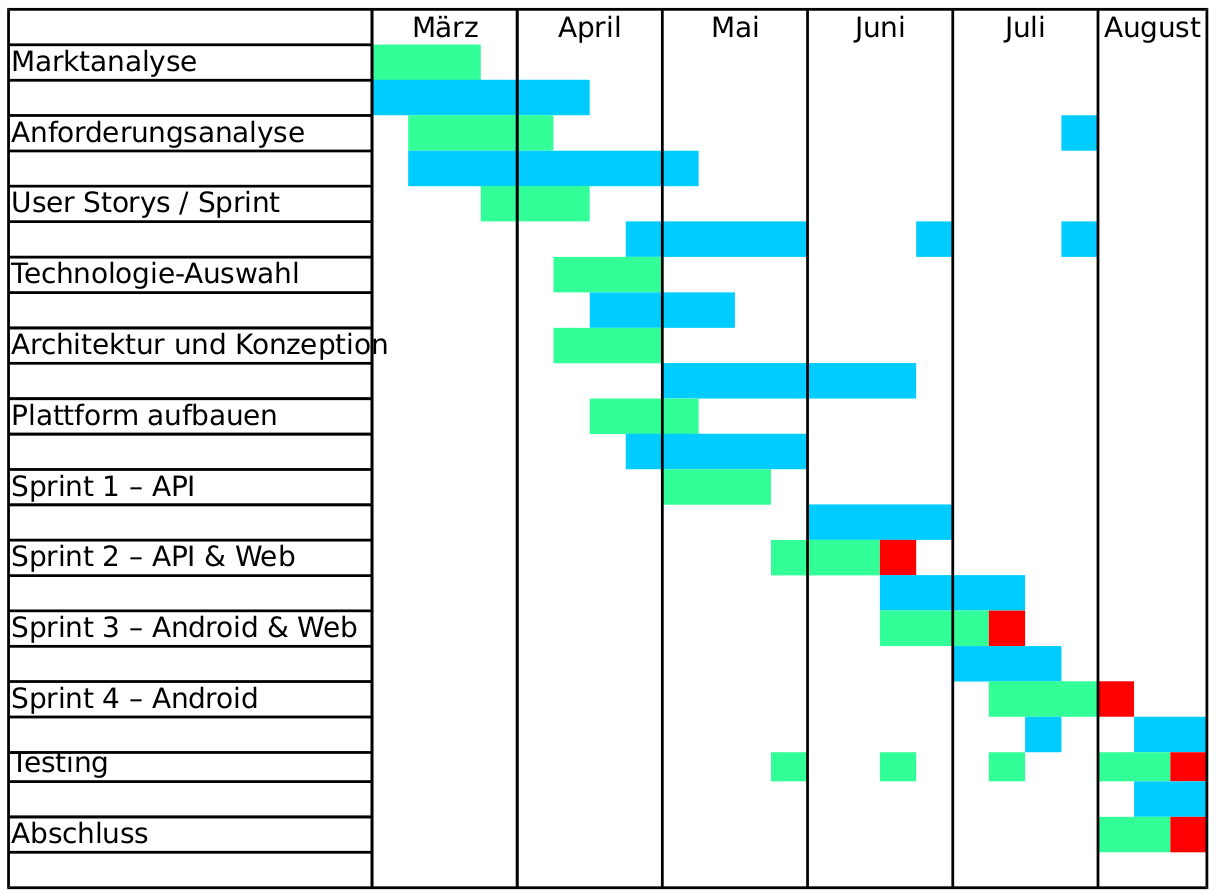
\includegraphics[width=1\textwidth, ]{Graphics/Grobplanung.png}
	\caption{Grobplanung f�r Applikation}
	\label{fig1}
\end{figure}





% !TeX spellcheck = de_DE
\chapter{Analyse}
Das Ziel der Software ist, den User in der Terminfindung, Protokollierung und Partnerfindung optimal zu unterst�tzen. Dieser Teil der Dokumentation dient zur Findung exakter Anforderungen an die Software, die den User optimal unterst�tzen. Zus�tzlich wird Anfangs untersucht wie das Marktumfeld rund um die geplante Applikation aussieht, um einen m�glichen Erfolg einer solchen Applikation zu sch�tzen sowie m�gliche Synergieeffekte zu identifizieren. 

\section{Marktumfeld}
Um m�gliche Synergien oder Wettbewerber zu identifizieren, m�ssen zuerst die geplanten Basis Funktionalit�ten aufgelistet werden:
\begin{itemize}
	 \itemsep-0.5em
	 \item Vereinfachung zur Identifizierung von Partnern
	 \item Vereinfachung zur Terminvereinbarung
	 \item Vereinfachung eines Amateur-Liga Management
	 \item Vereinfachung zu Protokollierung eines Spiels
	 
\end{itemize}

\subsection{Identifizierung von Partnern}
\textbf{GlobalTennisNetwork.com} ist eine Community zur Identifizierung von Tennispartnern. Die Website ist fokussiert auf Tennis. Andere Racket Sportarten werden nicht behandelt. Dadurch sieht der Autor dieser Service nicht als direkte Konkurrenz. Eine Verbindung mit dem Service um eine Gr�ssere Population von Potenziellen Tennispartnern zu erreichen w�re vorstellbar.
\\
\textbf{Spontacts} ist eine Android Applikation, welche Spontane Terminvereinbarungen erm�glicht. Es kann zus�tzlich als Identifizierung von Partnern f�r jegliche Freizeitaktivit�ten dienen. Es gibt jedoch keine Fokussierung auf Racket Sport. Nichts desto trotz kann Spontacts als konkurrenz zu der geplanten Applikation angesehen werden, da zwei Funktionalit�ten (auch wenn der Fokus nicht auf Sport liegt teilweise abgedeckt werden k�nnen. Jedoch 
wird die Konkurrenz nicht als erheblich eingesch�tzt. 
\\
\textbf{sport42.com} bietet auch eine M�glichkeit zur Identifizerung eines Portenziellen Sportpartners. Racket Sportarten werden hier auch abgedeckt. Nach Recherchen stellte sich jedoch heraus, das der Fokus der Applikation auf dem US Markt liegt. Bei einer potenziellen Expansion der geplanten Applikation m�sse die Konkurrenz neu evaluiert werden. Da der Fokus jedoch im Moment auf den deutschsprachigen Raum gerichtet ist, wird dieser Service nicht als Konkurrenz eingesch�tzt. 
\\
\textbf{sportpartner.com} ist ein auf Sport fokussierter Service um Partner zu identifizieren. Der Service deckt auch Racketsportarten wie Tennis, Squash sowie Badminton ab. Bis jetzt gibt es allerdings nur wenig aktive Spieler in Europa.
\\
\subsection{Terminvereinbarung}
 \textbf{Doodle} ist der bekannteste Terminvereinbarungs Service. Ein �hnlicher Algorithmus, welcher in der geplanten Applikation verwendet wird, wurde von den Ersteller dieser Applikation entwickelt. Jedoch gibt es bei Doodle keinerlei Fokus auf Inhalt zum Termin. Es ist m�glich Business wie auch Freizeit Termine zu erstellen. Die geplante Applikation kann davon Profitieren einen �hnlichen, auf Sport Termine fokussierte Terminvereinbarungs Algorithmus zu entwickeln. Sollte dieser gen�gend intuitiv Umgesetzt sein, wird Doodle nicht als Konkurrenz betrachtet. \\
 \textbf{Moreganize.ch} wie Doodle ben�tzt auch Moreganize einen Terminvereinbarungs Algorithmus. 
 

\subsection{Amateur-Liga Management}
\textbf{LeagueManager Wordpress Plugin} ist eine Zusatzsoftware f�r Wordpress, mit welchen man Teams und Matches zusammenstellen kann und so Ligen erstellen kann. Der Fokus liegt hier gr�sstenteils auf Teamsports.

\textbf{Excel} von Microsoft wird oft als Tracking und Organisation f�r Ligen verwendet. Die Einfachheit und das breite Skillset spricht f�r diese L�sung. Jedoch ist Zusammenarbeit und Organisation umst�ndlich.

\subsection{Protokollierung eines Spiels}
\textbf{Excel} von Microsoft wird oft als Tracking und Organisation f�r Ligen verwendet. Die Einfachheit und das breite Skillset spricht f�r diese L�sung. Jedoch ist Zusammenarbeit und Organisation umst�ndlich. Als alternative, welche die Zusammenarbeit vereinfacht bietet sich auch \textbf{Google Docs} an.


\section{Benutzergruppen/Ist-Analyse}
Die geplante Applikation wird nicht f�r alle Benutzergruppen interessant sein. Um das Zielklientel zu finden wird  erstellt diese Kapitel eine Kategorisierung in verschiedene Benutzergruppen. Anschliessend wird abgesch�tzt, wie welche Benutzergruppe von der Applikation profitieren kann. 

\subsection{Gelegenheitsspieler}
\subsubsection{Analyse}
Gelegenheitsspieler spielen nicht regelm�ssig (w�chentlich) Racketsport. Sie vereinbaren mit - meistens wenige Personen in engem oder erweitertem privaten Umfeld - unregelm�ssig Spiele. Oft pausieren Gelegenheitsspieler mehrere Monate und haben anschliessend intensivere Phasen mit mehreren Spielen innerhalb wenigen Wochen. Der Aufwand um ein Spiel zu vereinbaren und einen passenden Court zu finden ist dementsprechend gross. Viel fehlt auch an einem passenden Partner im privaten Umfeld, insbesondere wenn der Spieler Ambitionen hegt sich zu verbessern. Schlussendlich ist die Motivation zu einer \glqq gewissen Regelm�ssigkeit \grqq nicht hoch, da die Vereinbarung eines Spieles aufw�ndig ist, sowie eine Verbesserung des Spiels gegen�ber anderen Spielern nicht schnell ersichtlich ist.\\
Zusammengefasst lassen Sich folgende Charakteristiken zusammenfassen:
\begin{itemize}[nosep]
	\item Einzelne oder wenige Partner im privatem Umfeld
	\item Oft l�ngere Pausen gefolgt von intensiveren Phasen
	\item Grosse Aufwand um Spiel zu vereinbaren
	\item Fehlende Partner bei gewollter Verbesserung im Spiel
	\item Fehlende Vergleichsm�glichkeiten, da wenige Partner und meist keine Protokollierung der Ergebnisse
	\item Wenig Anreize um n�chstes Spiel zu organisieren
\end{itemize}

\subsubsection{Use Cases}
Gelegenheitsspieler k�nnen ausserordentlich von der geplante Applikation profitieren. \\
Neue \textbf{Partner} in der N�he k�nnen unkompliziert mit der Applikation identifiziert werden. So ist es m�glich l�ngere Pausen, wenn der originale Partner in den Ferien ist oder schlicht verhindert ist, zu verhindern.
\\
\textbf{Courts und Spielzeiten} k�nnen schnell vereinbart werden. Dies verringert den Aufwand um ein Spiel durchzuf�hren und erh�ht somit die Motivation �fters Squash zu spielen.
Spiele k�nnen \textbf{protokolliert} werden und so kann eine Statistik erstellt werden, welche wiederum als Anreiz dienen kann um besser zu werden.\\
Durch ein \textbf{Liga Management} k�nnen zus�tzliche Anreize, neue Partner sowie eine Regelm�ssigkeit gefunden werden. M�glicherweise sind ein Grossteil der Gelegenheitsspieler nicht an einer solchen Liga interessiert, jedoch gibt es ein gewisses Potenzial daf�r.



\subsection{Regelm�ssige Spieler}
\subsubsection{Analyse}
Regelm�ssige Spieler spielen regelm�ssig zu einem vereinbarten Termin mit einem oder mehreren Partner einen Racketsport. Meist werden genannte vereinbarte Termine mit den gleichen Partnern ausgetragen. Bei den vereinbarten Terminen gibt es gewisse Variationen. So kann der Zeitpunkt und auch der Wochentag variieren. 

Zus�tzlich zu den regelm�ssigen Terminen, kommen  meist noch unregelm�ssige Termine in der Charakteristik der Gelegenheitsspieler hinzu. 

Durch die Regelm�ssigkeit ist diese Spielergruppe meist einiges ambitionierter als Gelegenheitsspieler. Dadurch das Sie regelm�ssig mit den gleichen Spielern spielen, wollen Sie besser sein als die anderen. Da Sie jedoch nicht in einer Liga spielen gibt es meist kein Protokoll der Resultate oder ein Ranking.

\subsubsection{Use Cases}
Regelm�ssige Spieler k�nnen durch die geplante Applikation sehr unkompliziert ihre Spiele \textbf{protokollieren}. 
\\
Eine \textbf{Liga} kann zwischen mehreren regelm�ssigen Spielern arrangiert werden. Diese kann durch regelm�ssige \textbf{Terminvereinbarungen vom System} dazu beitragen das es keine Pausen gibt bei Krankheit oder Abwesenheit. Spieler die ausserhalb der eigenen Stammgruppe spielen wollen, k�nnen gleichzeitig bei \textbf{�ffentlichen Ligen} weitere Erfahrungen sammeln.



\subsection{Clubmitglieder}
\subsubsection{Analyse}
Clubmitglieder Spielen regelm�ssig und haben daf�r fix Vereinbarte Clubtrainings. Diese sind nicht flexibel. Zus�tzlich besteht auch eine Infrastruktur f�r Ranking �ber die Liga sowie eine Protokollierung von Spielen in den meisten F�llen.	Clubmitglieder sind somit nicht im Hauptfokus dieser Applikation. H�chstens Ausserhalb des Clublebens ist es gut m�glich das ein Clubmitglied diese Applikation braucht um neue Spiele zu vereinbaren oder in einer privaten Liga mitzuspielen. 

\subsubsection{Use Cases}
Neue Clubs ohne Infrastruktur k�nnten diese Applikation f�r ihre Administration verwenden.
\newpage
\section{Anforderungsanalyse}

\subsection{Vision}
Erleichterung zur Terminfindung und Administration von Racketsportspieleren

\subsection{Ziele}
Folgende Business Prozesse sollten unterst�tzt werden:
\begin{itemize}
	\itemsep -0.2em
 \item Identifizierung von Partnern
 \item Terminvereinbarung
 \item Amateur-Liga Management
 \item Protokollierung eines Spiels
\end{itemize}


\subsection{Rahmenbedingungen}
\subsubsection{Allgemein}
Die Applikation hat keine konkreten Rahmenbedingungen. Sie ist eine Standalone Applikation und hat keine externen Abh�ngigkeiten. 
\subsubsection{Technologie}
Es gibt keine Einschr�nkungen, welche Technologie benutzt werden sollte, solange die Anforderungen erf�llt werden.
\subsubsection{Erweiterbarkeit}
Die Applikation soll m�glicht einfach erweiterbar sein. Zus�tzliche Sicherheit, neue Funktionalit�ten sowie skalierbarkeit in Performance sowie Stabilit�t sollten mit der eingesetzten Technologie m�glich sein. 
\subsubsection{Sicherheit}
Technologien sollten Stanard Sicherheitsanforderungen im Web umsetzen k�nnen. Privacy und Integrity Anforderungen sind in diesem Proof of Concept noch nicht geplant.
\subsubsection{Stabilit�t und Performance}
F�r den Proof of Concept sind keine Stabilit�ts- und Performance Anforderungen n�tig. 
\newpage
\subsection{Schnittstellen}
Folgende Tabelle zeigt interne sowie externe Schnittstellen auf:
\begin{center}
	\tabulinesep = 1mm
	\begin{longtabu} to \linewidth [m]{|[2pt]p{1cm}|[2pt]p{3cm}|[2pt]X[1, m , l]|[2pt]}
		\arrayrulecolor{white}
		
		\tabucline[2pt]{-}
		\textcolor{white}{\textbf{\cellcolor{airforceblue}ID}}  &  
		\textcolor{white}{\textbf{\cellcolor{airforceblue}Name	}}&
		\textcolor{white}{\textbf{\cellcolor{airforceblue}Beschreibung	}}
		\tabularnewline
		\tabucline[2pt]{-}
		\textcolor{white}{\textbf{\cellcolor{airforceblue}I1}} &
		\cellcolor{testblau}  API $\longrightarrow$ Client &
		\cellcolor{testblau}Der Client greift auf die API zu um die aktuellen Daten dem Benutzers anzuzeigen. API sollte HTTP REST benutzen.
		\tabularnewline
		\tabucline[2pt]{-}
		\textcolor{white}{\textbf{\cellcolor{airforceblue}I2}} &
		\cellcolor{testblau}  Client $\longrightarrow$ Browser &
		\cellcolor{testblau}Der Client l�uft innerhalb eines Browsers. Der Browser f�hrt die Applikation - bestehend aus HTML, CSS und Javascript - aus. 
		\tabularnewline
		\tabucline[2pt]{-}
		\textcolor{white}{\textbf{\cellcolor{airforceblue}I3}} &
		\cellcolor{testblau}  Browser $\longrightarrow$ Android &
		\cellcolor{testblau}Der Browser l�uft innerhalb der Android Applikation. Die Android Applikation Emuliert den Browser und zeigt die Applikation als App dem Benutzer an.
		\tabularnewline
		\tabucline[2pt]{-}
		\tabucline[2pt]{-}
	\end{longtabu}\end{center}

\FloatBarrier


\subsection{Anwendungsf�lle}


\subsubsection{UC0 - Login in das System}

\begin{center}
	
	
	\tabulinesep = 1mm
	\begin{longtabu} to \linewidth [m]{|[2pt]p{3cm}|[2pt]X[1, m , l]|[2pt]}
		\arrayrulecolor{white}
		
		\tabucline[2pt]{-}
		\textcolor{white}{\textbf{\cellcolor{airforceblue}UC0}}  &   
		\textcolor{white}{\textbf{\cellcolor{airforceblue}Login in das System	}}
		\tabularnewline
		\tabucline[2pt]{-}
		\textcolor{white}{\textbf{\cellcolor{airforceblue}Beschreibung}} &  
		\cellcolor{testblau}{Ein User des Systems will sich mit dem System authentisieren. Der Benutzer bekommt durch die Authentisierung Autorisierungen zugesprochen sowie ein Profil und Daten zugeordnet. Es erm�glicht dem User seine eigene Ansicht in die Daten des Systems zu erhalten. Da dieses System eine Applikation individualisiert f�r den User darstellt, sind alle Ansichten in das System einer Autorisierung zugeordnet und k�nnen nur von authentisierten Benutzern benutzt werden.}
		\tabularnewline
		\tabucline[2pt]{-}
		\textcolor{white}{\textbf{\cellcolor{airforceblue}Diagramm}} & 	\cellcolor{testblau}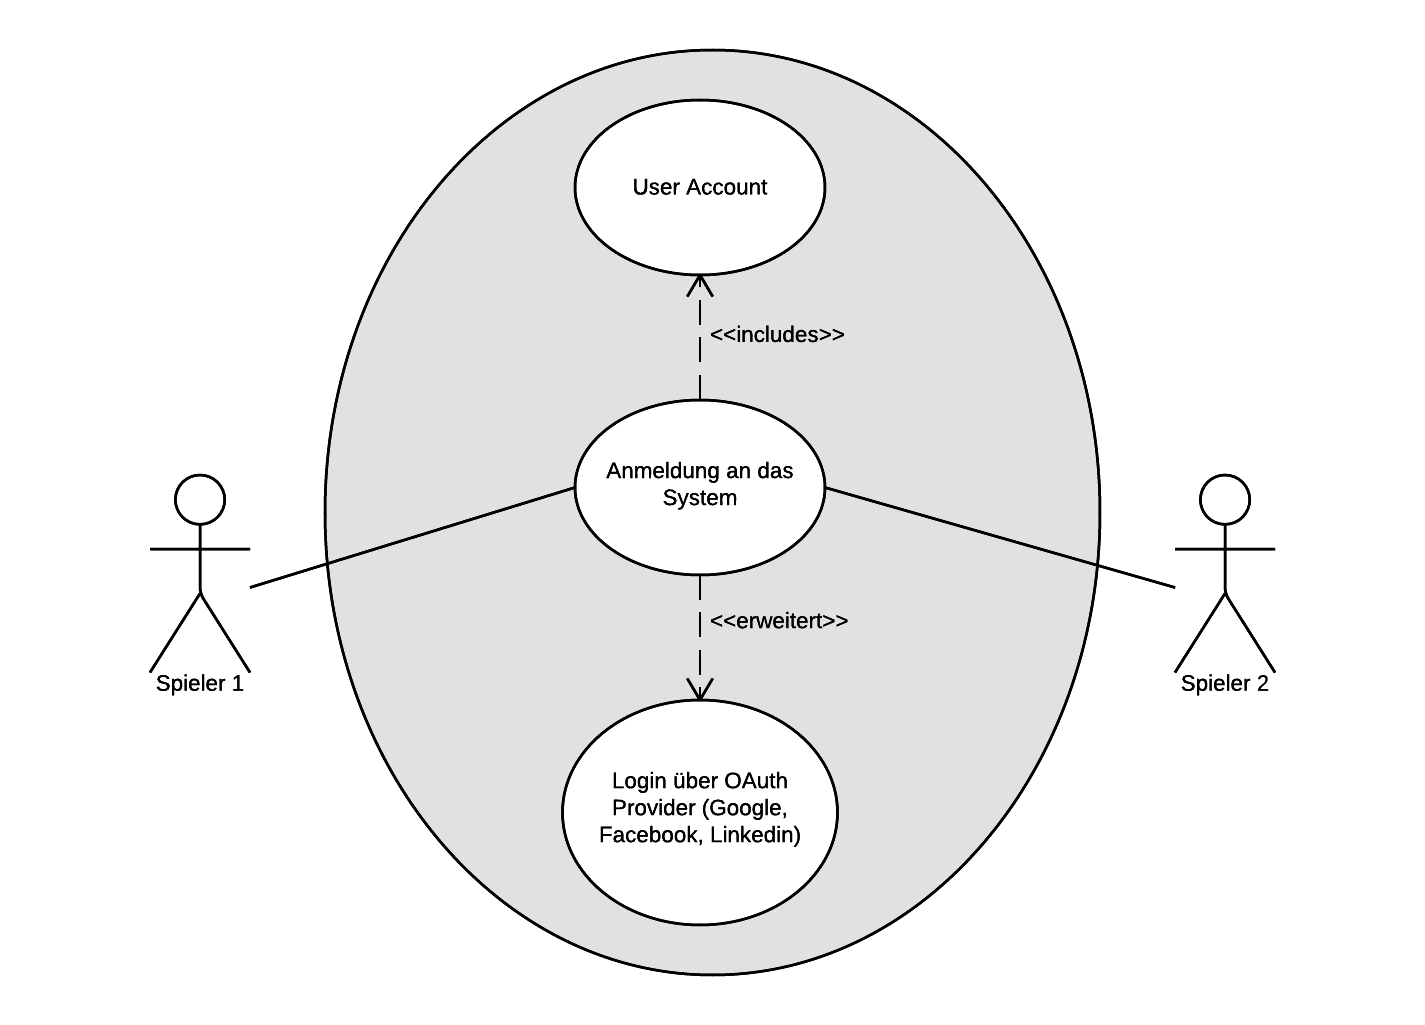
\includegraphics[width=0.7\textwidth]{Graphics/UC0.png}
		\tabularnewline
		\tabucline[2pt]{-}
		\textcolor{white}{\textbf{\cellcolor{airforceblue}Version}} &
		\cellcolor{testblau} 1.0
		\tabularnewline
		\tabucline[2pt]{-}
		\textcolor{white}{\textbf{\cellcolor{airforceblue}Vorbedingung}} &
		\cellcolor{testblau} -
		\tabularnewline
		\tabucline[2pt]{-}
		\textcolor{white}{\textbf{\cellcolor{airforceblue}Anforderungen}} &
		\cellcolor{testblau}
		\begin{tabular}[x]{@{}l@{}}
			REQ0.01 - Anmeldung an das System\\
			REQ0.02 - Registrierung eines Users mit dem System\\
			REQ0.03 - Authentisierung �ber OAuth 
			\end{tabular}
			\tabularnewline
			\tabucline[2pt]{-}
			\textcolor{white}{\textbf{\cellcolor{airforceblue}Testf�lle}} &
			\cellcolor{testblau}	
			\begin{tabular}[x]{@{}l@{}}
				Test0.1: Anmeldung �ber Username/Passwort\\
				Test0.2: Anmeldung �ber OAuth\\
				Test0.3: Registrierung �ber Username/Passwort\\
				Test0.4: Registrierung �ber OAuth
				\end{tabular}  
				\tabularnewline
				\tabucline[2pt]{-}
				\textcolor{white}{\textbf{\cellcolor{airforceblue}
						\begin{tabular}[x]{@{}l@{}}
							Standard\\
							Sequenz
							\end{tabular}}} & 	\cellcolor{testblau}		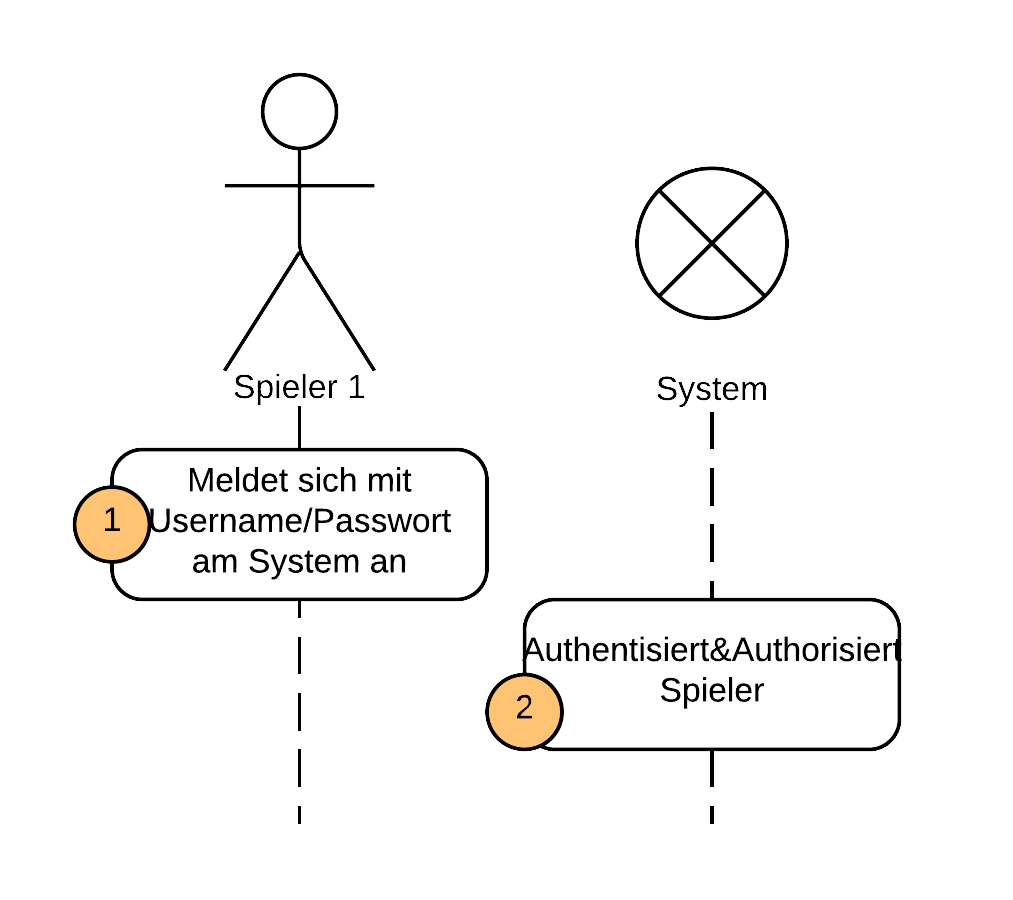
\includegraphics[width=0.5\textwidth]{Graphics/SEQSUC0.png}
							\tabularnewline
							\tabucline[2pt]{-}
							\textcolor{white}{\textbf{\cellcolor{airforceblue}Alternative Sequenzen}} & \cellcolor{testblau}
							\begin{tabular}[x]{@{}c@{}}
									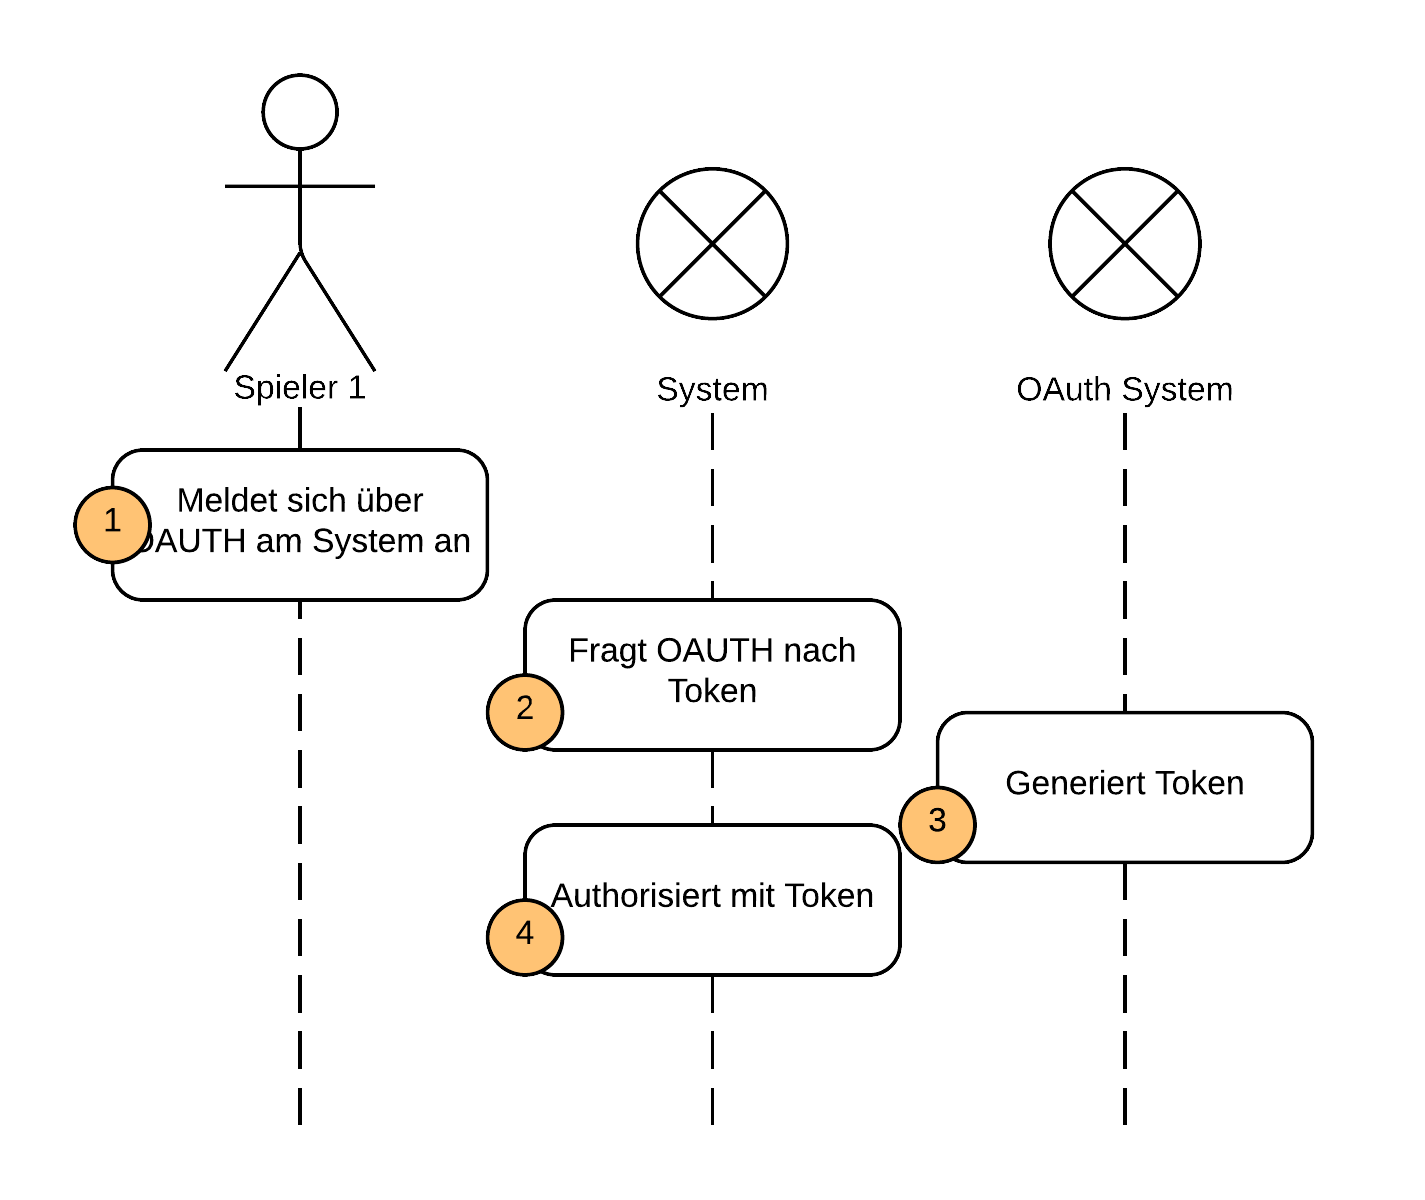
\includegraphics[width=0.4\textwidth]{Graphics/SEQA1UC0.png}\\
									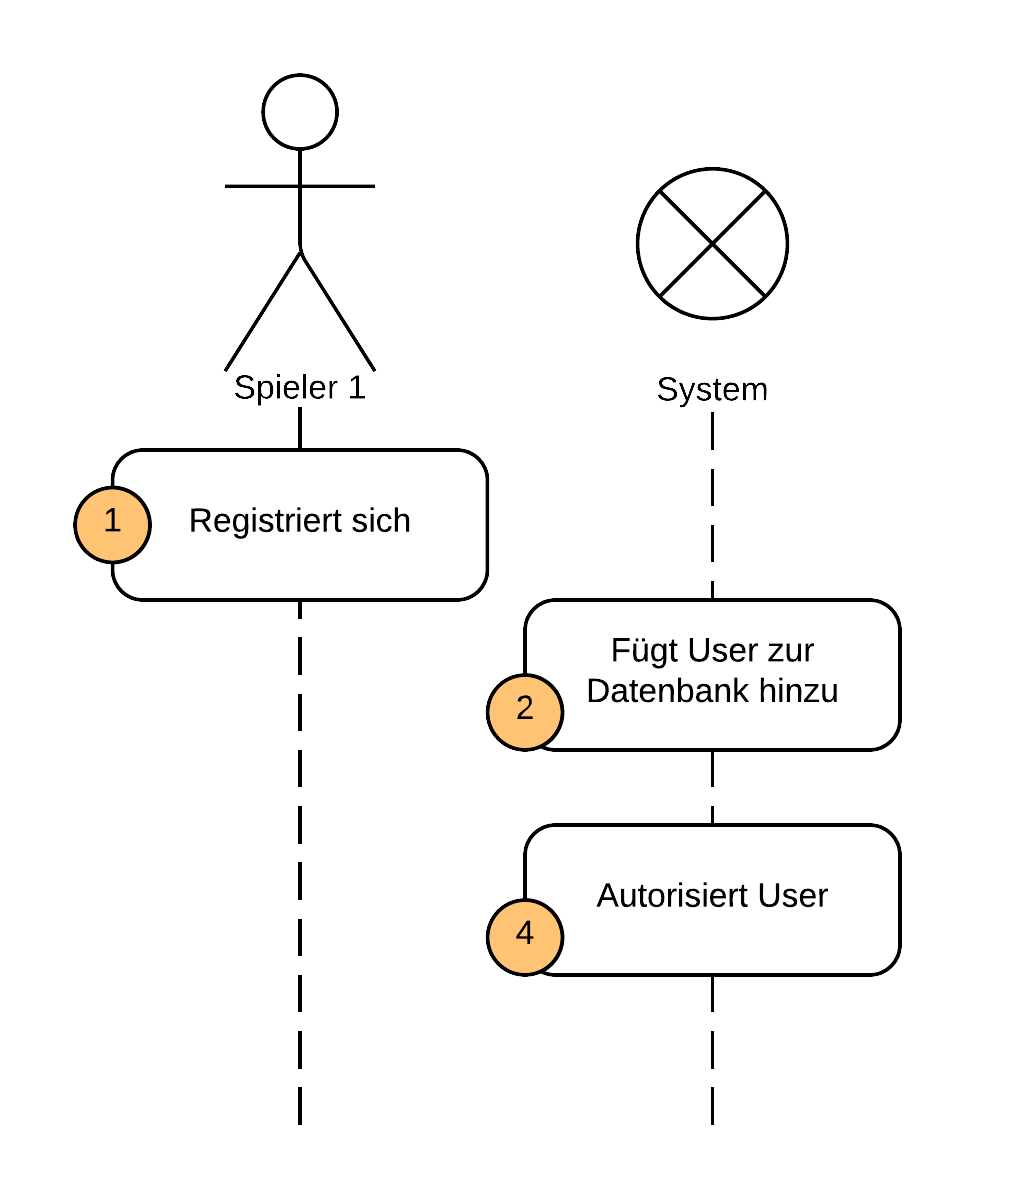
\includegraphics[width=0.4\textwidth]{Graphics/SEQA2UC0.png}
							\end{tabular}
						
							\tabularnewline
							\tabucline[2pt]{-}
							
							
							\end{longtabu}
			\newpage				
							\end{center}

\subsubsection{UC1 - Identifizierung von Partnern}
\begin{center}
	
	
	\tabulinesep = 1mm
	\begin{longtabu} to \linewidth [m]{|[2pt]p{3cm}|[2pt]X[1, m , l]|[2pt]}
		\arrayrulecolor{white}
		
		\tabucline[2pt]{-}
		\textcolor{white}{\textbf{\cellcolor{airforceblue}UC1}}  &   
		\textcolor{white}{\textbf{\cellcolor{airforceblue}Identifizierung von Partnern }}
		\tabularnewline
		\tabucline[2pt]{-}
		\textcolor{white}{\textbf{\cellcolor{airforceblue}Beschreibung}} &  
		\cellcolor{testblau}{Zwei Partner - A und B - wollen einen bestimmten Racketsport in einer bestimmten Region spielen. Der User A oder B kann Spielvorschl�ge an andere User senden. Daf�r kann er nach Region filtern.}
		\tabularnewline
		\tabucline[2pt]{-}
		\textcolor{white}{\textbf{\cellcolor{airforceblue}Diagramm}} & 	\cellcolor{testblau}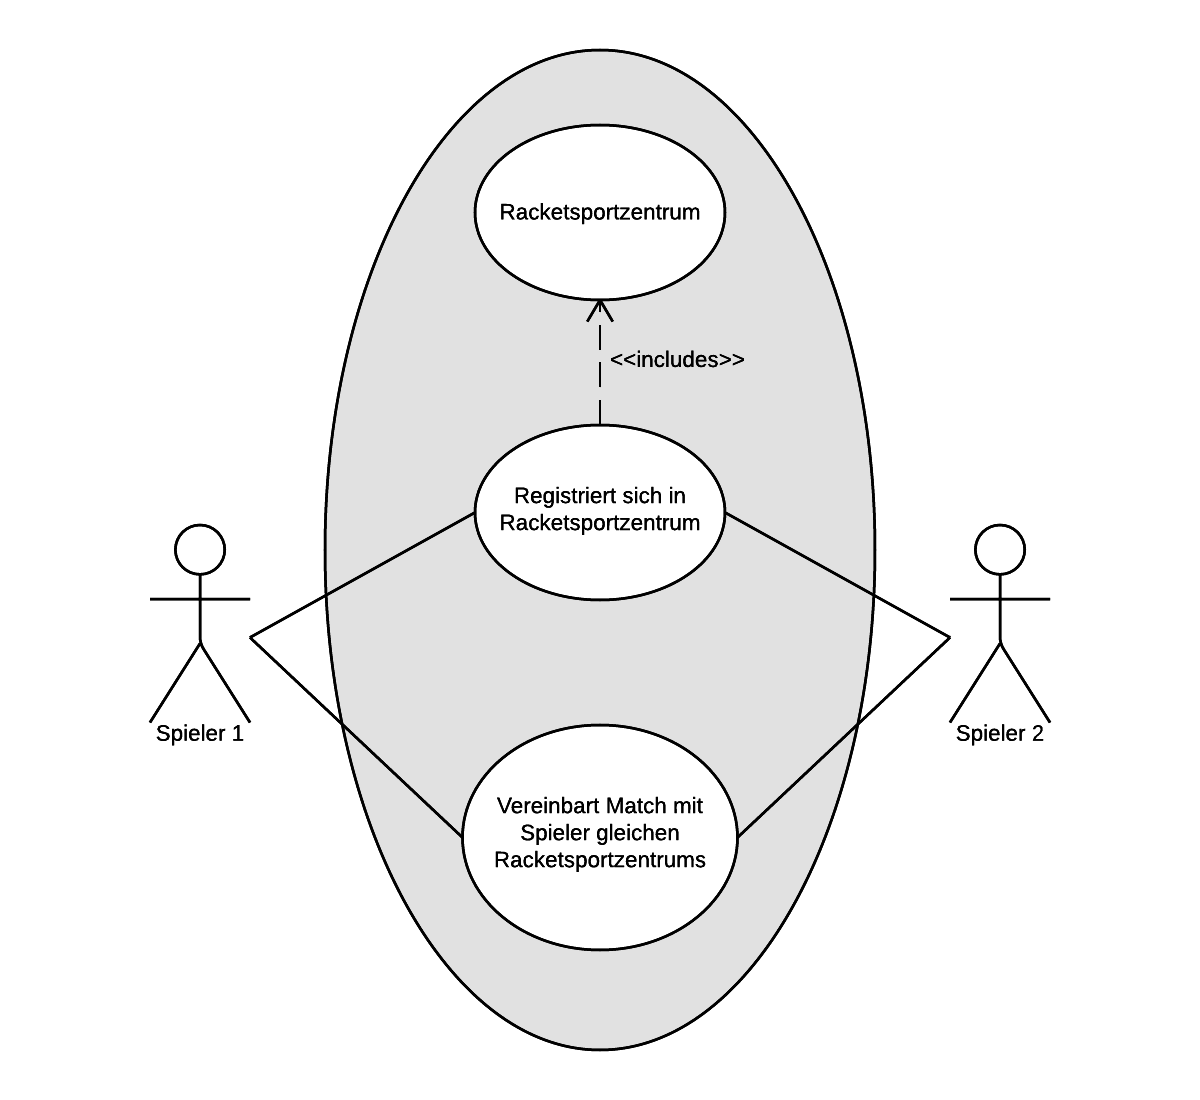
\includegraphics[width=0.7\textwidth]{Graphics/UC1.png}
		\tabularnewline
		\tabucline[2pt]{-}
		\textcolor{white}{\textbf{\cellcolor{airforceblue}Version}} &
		\cellcolor{testblau} 1.0
		\tabularnewline
		\tabucline[2pt]{-}
		\textcolor{white}{\textbf{\cellcolor{airforceblue}Vorbedingung}} &
		\cellcolor{testblau} UC0 - Anmeldung an das System
		\tabularnewline
		\tabucline[2pt]{-}
		\textcolor{white}{\textbf{\cellcolor{airforceblue}Anforderungen}} &
		\cellcolor{testblau}
		\begin{tabular}[x]{@{}l@{}}
			REQ1.01 - Zuteilung von User zu Racketsportzentren\\
			REQ1.02 - Details zu Spielern\\
			REQ1.03 - Friend System\\
			REQ3.01 - Court erstellen \\
			REQ3.02 - Spieler k�nnen sich in Courts eintragen
		\end{tabular}
		\tabularnewline
		\tabucline[2pt]{-}
		\textcolor{white}{\textbf{\cellcolor{airforceblue}Testf�lle}} &
		\cellcolor{testblau}	
		\begin{tabular}[x]{@{}l@{}}
			Test1.1: TBD\\
			Test 1.2: TBD
		\end{tabular}  
		\tabularnewline
		\tabucline[2pt]{-}
			\textcolor{white}{\textbf{\cellcolor{airforceblue}
					\begin{tabular}[x]{@{}l@{}}
						Standard\\
						Sequenz
						\end{tabular}}} & 	\cellcolor{testblau}		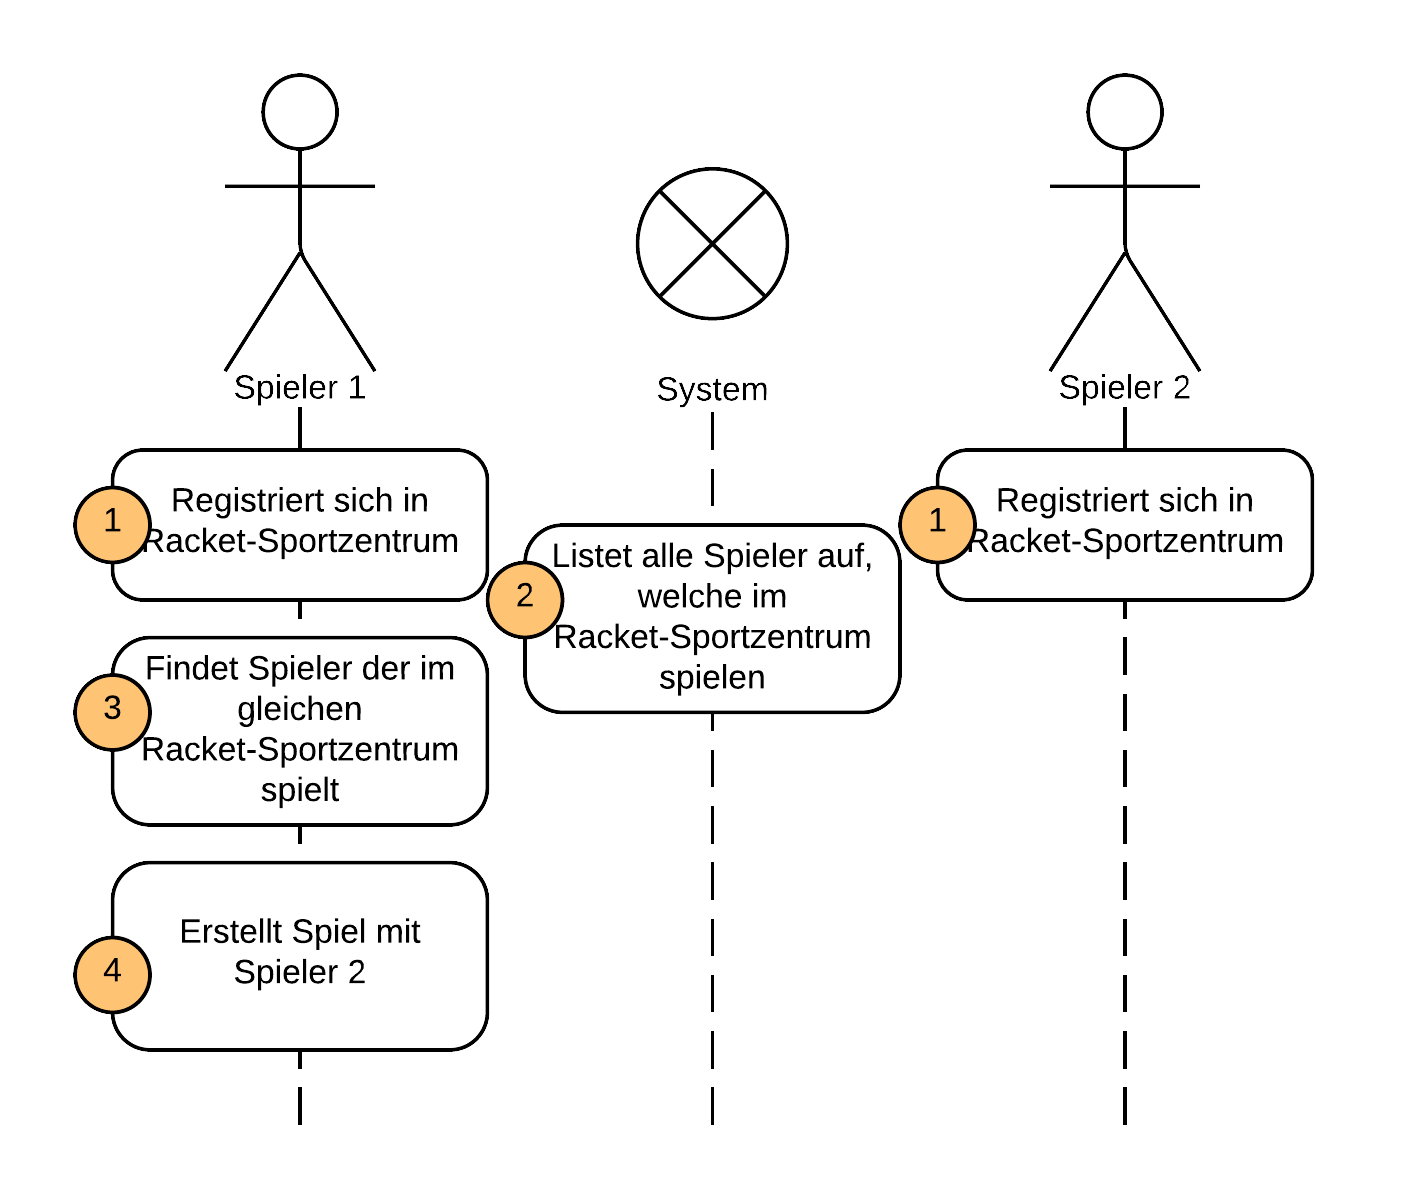
\includegraphics[width=0.7\textwidth]{Graphics/SEQSUC1.png}
			\tabularnewline
			\tabucline[2pt]{-}
		
			
		
	\end{longtabu}
	
\end{center}
\FloatBarrier
\newpage
\subsubsection{UC2 - Terminvereinbarung}

\begin{center}
	
	
	\tabulinesep = 1mm
	\begin{longtabu} to \linewidth [m]{|[2pt]p{3cm}|[2pt]X[1, m , l]|[2pt]}
		\arrayrulecolor{white}
		
		\tabucline[2pt]{-}
		\textcolor{white}{\textbf{\cellcolor{airforceblue}UC2}}  &   
		\textcolor{white}{\textbf{\cellcolor{airforceblue}Terminvereinbarung }}
		\tabularnewline
		\tabucline[2pt]{-}
		\textcolor{white}{\textbf{\cellcolor{airforceblue}Beschreibung}} &  
		\cellcolor{testblau}{Der Spieler A kann einen oder mehrere Spielvorschl�ge senden. Anschliessend kann der Spieler B einer dieser Spielvorschl�ge \textbf{annehmen}, \textbf{ablehnen} oder \textbf{neue Spielvorschl�ge senden}. Sobald beide Nutzer einen Spielvorschlag angenommen hat, gilt der Termin als vereinbart. }
		\tabularnewline
		\tabucline[2pt]{-}
		\textcolor{white}{\textbf{\cellcolor{airforceblue}Diagramm}} & 	\cellcolor{testblau}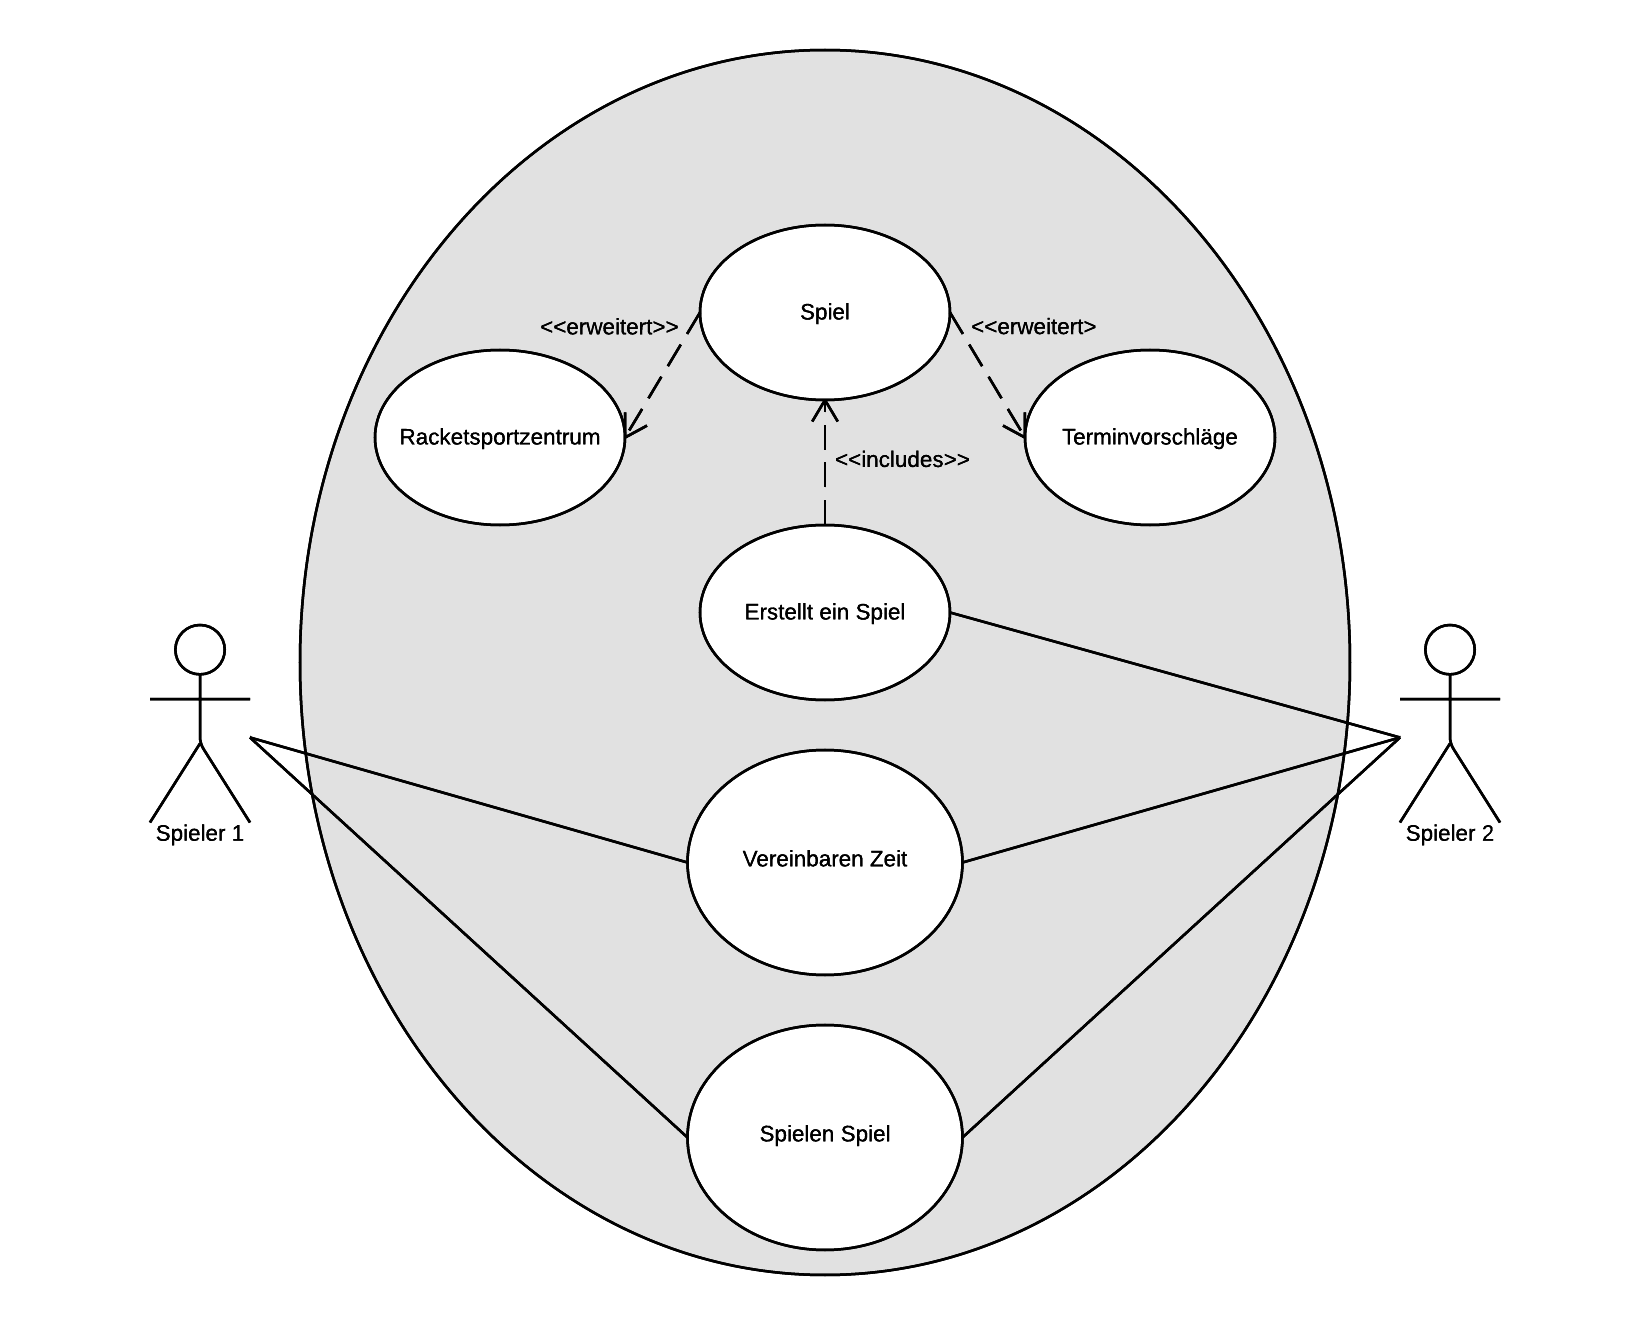
\includegraphics[width=0.8\textwidth]{Graphics/UC2.png}
		\tabularnewline
		\tabucline[2pt]{-}
		\textcolor{white}{\textbf{\cellcolor{airforceblue}Version}} &
		\cellcolor{testblau} 1.0
		\tabularnewline
		\tabucline[2pt]{-}
		\textcolor{white}{\textbf{\cellcolor{airforceblue}Vorbedingung}} &
		\cellcolor{testblau} UC0 - Anmeldung an das System
		\tabularnewline
		\tabucline[2pt]{-}
		\textcolor{white}{\textbf{\cellcolor{airforceblue}Anforderungen}} &
		\cellcolor{testblau}
		\begin{tabular}[x]{@{}l@{}}
			REQ2.01 - Spiel erstellen \\
			REQ2.02 - Spielterminvorschl�ge erstellen\\
			REQ2.03 - Spielterminvorschl�ge annehmen und ablehnen\\
			REQ2.04 - Wiederkehrende Spiele erstellen\\
			REQ2.06 - Privatsph�reeinstellungen ber�cksichtigen
		\end{tabular}
		\tabularnewline
		\tabucline[2pt]{-}
		\textcolor{white}{\textbf{\cellcolor{airforceblue}Testf�lle}} &
		\cellcolor{testblau}	
		\begin{tabular}[x]{@{}l@{}}
			Test2.1: TBD\\
			Test2.2: TBD
		\end{tabular}  
		\tabularnewline
		\tabucline[2pt]{-}
		\textcolor{white}{\textbf{\cellcolor{airforceblue}
				\begin{tabular}[x]{@{}l@{}}
					Standard\\
					Sequenz
				\end{tabular}}} & 	\cellcolor{testblau}		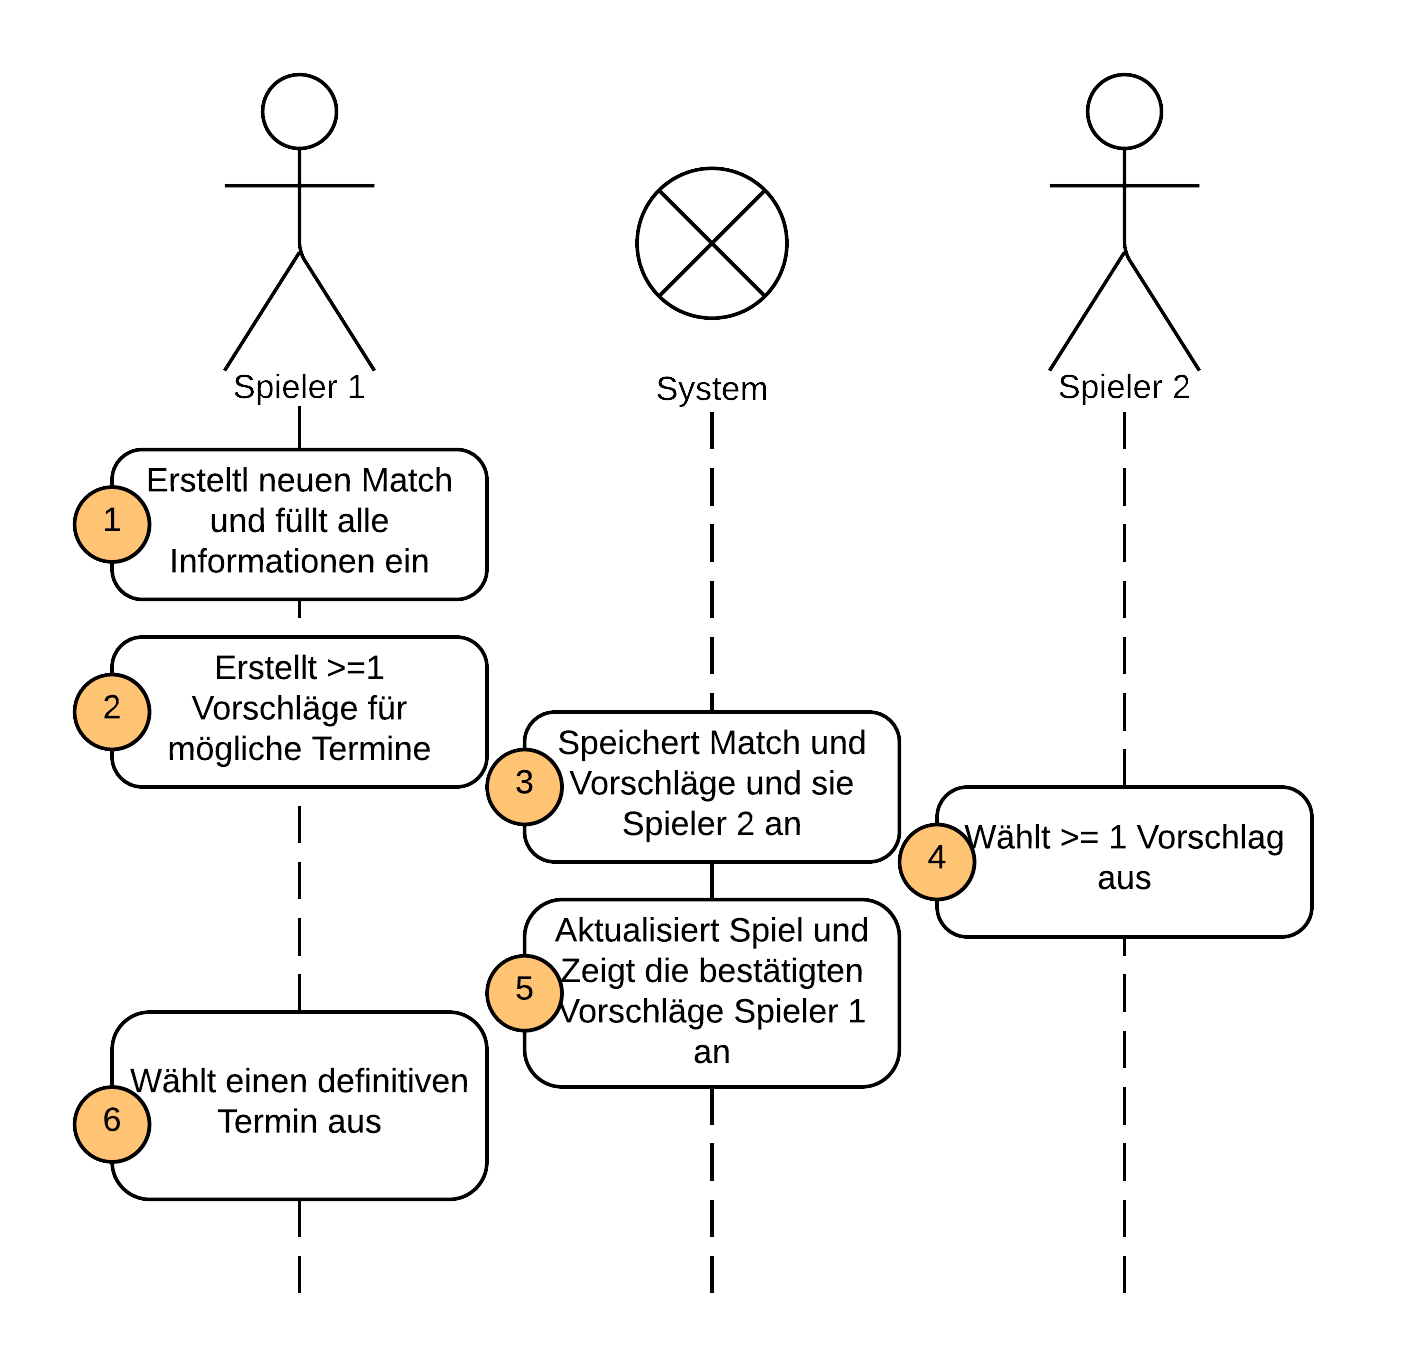
\includegraphics[width=0.7\textwidth]{Graphics/SEQSUC2.png}
				\tabularnewline
				\tabucline[2pt]{-}
					\textcolor{white}{\textbf{\cellcolor{airforceblue}Alternative Sequenzen}} & \cellcolor{testblau}
				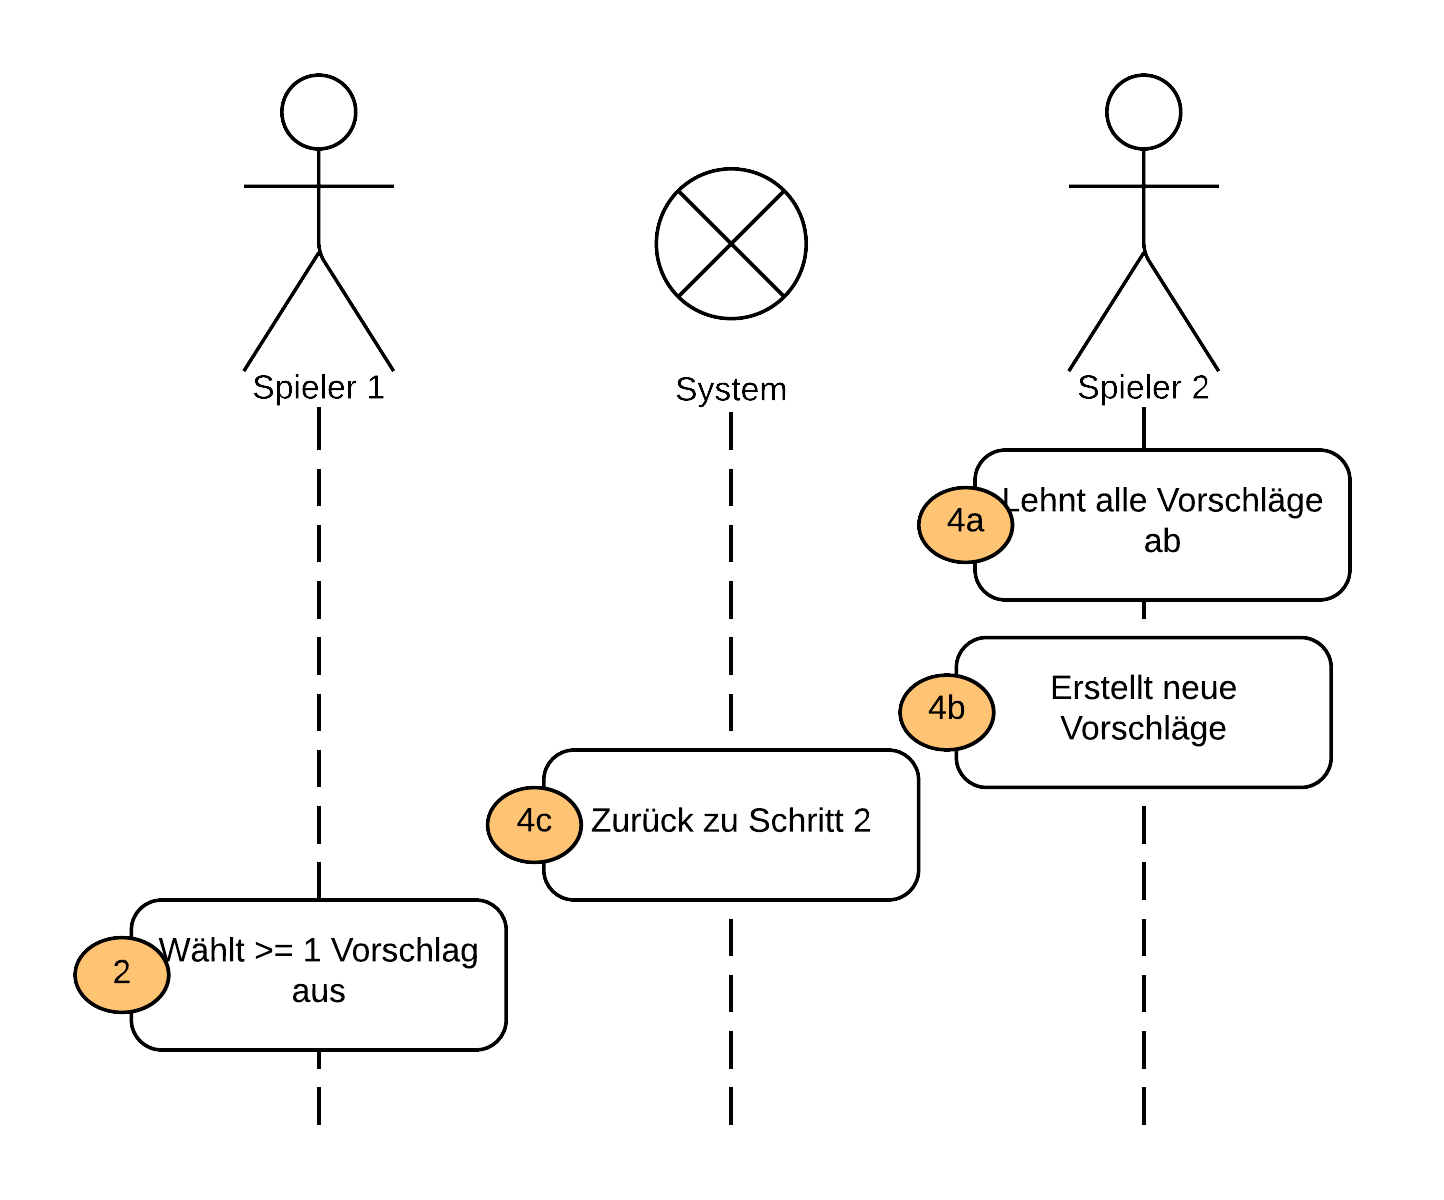
\includegraphics[width=0.7\textwidth]{Graphics/SEQA1UC2.png}
					\tabularnewline
					\tabucline[2pt]{-}
				
				
			\end{longtabu}
			
		\end{center}


\FloatBarrier

\newpage

\subsubsection{UC 3 - Spiel Protokollieren}

\begin{center}
	
	
\tabulinesep = 1mm
\begin{longtabu} to \linewidth [m]{|[2pt]p{3cm}|[2pt]X[1, m , l]|[2pt]}
		\arrayrulecolor{white}
		
		\tabucline[2pt]{-}
		\textcolor{white}{\textbf{\cellcolor{airforceblue}UC3}}  &   
		\textcolor{white}{\textbf{\cellcolor{airforceblue}Spiel protokollieren }}
		\tabularnewline
		\tabucline[2pt]{-}
		\textcolor{white}{\textbf{\cellcolor{airforceblue}Beschreibung}} &  
		\cellcolor{testblau}{Nachdem ein Spiel durchgef�hrt wurde, kann der Spieler B sowie der Spieler A die Scores eintragen oder best�tigen. Anschliessend k�nnen beide Spieler die jeweiligen vergangenen Spiele jederzeit in der Applikation nachschlagen. Optional wird das protokollierte Spiel in einer Liga gewertet (falls vor dem Spiel so deklariert. }
		\tabularnewline
		\tabucline[2pt]{-}
		\textcolor{white}{\textbf{\cellcolor{airforceblue}Diagramm}} & 	\cellcolor{testblau}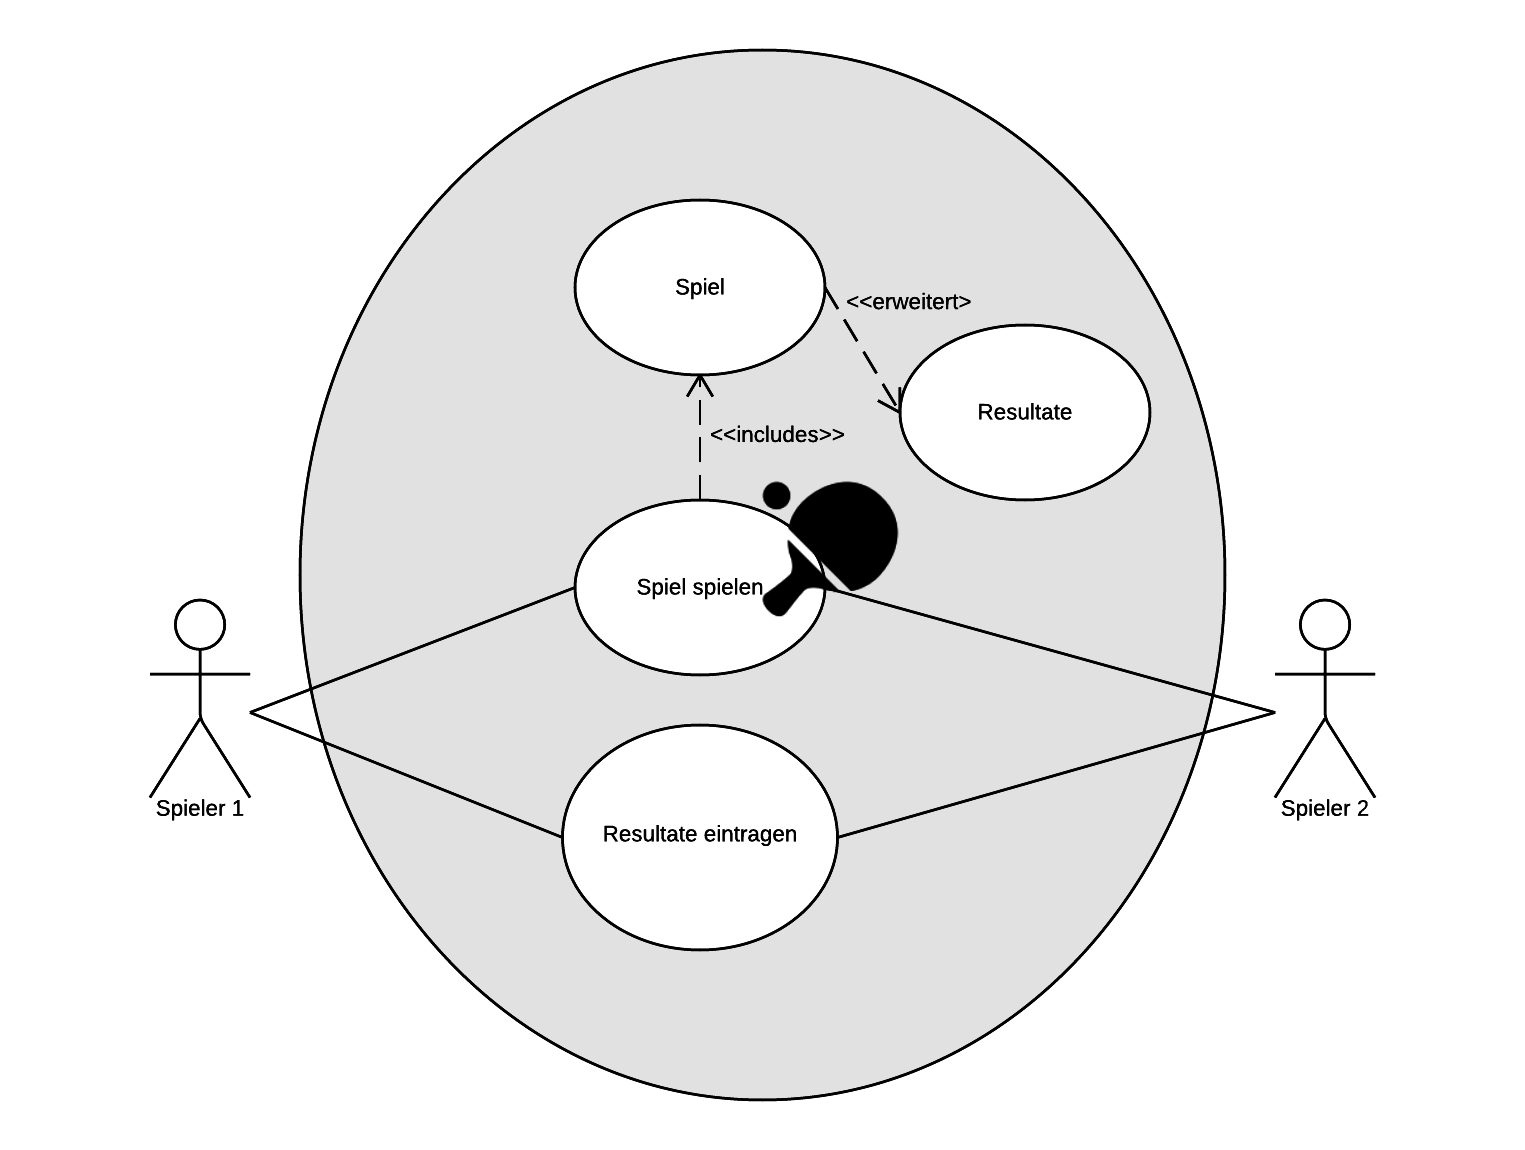
\includegraphics[width=0.8\textwidth]{Graphics/UC3.png}
		\tabularnewline
		\tabucline[2pt]{-}
		\textcolor{white}{\textbf{\cellcolor{airforceblue}Version}} &
		\cellcolor{testblau} 1.0
		\tabularnewline
		\tabucline[2pt]{-}
		\textcolor{white}{\textbf{\cellcolor{airforceblue}Vorbedingung}} &
		\cellcolor{testblau} 
		\begin{tabular}[x]{@{}l@{}}
			UC0 - Anmeldung an das System\\
			UC1 - Terminvereinbarung
		\end{tabular}
		\tabularnewline
		\tabucline[2pt]{-}
		\textcolor{white}{\textbf{\cellcolor{airforceblue}Anforderungen}} &
		\cellcolor{testblau}
		\begin{tabular}[x]{@{}l@{}}
			REQ2.07 - Ergebnissedes Spiels eintragen \\
			REQ2.08 - Best�tigung des Spiels eintragen
		
		\end{tabular}
		\tabularnewline
		\tabucline[2pt]{-}
		\textcolor{white}{\textbf{\cellcolor{airforceblue}Testf�lle}} &
		\cellcolor{testblau}	
		\begin{tabular}[x]{@{}l@{}}
			Test3.1: TBD\\
			Test1.2: TBD
		\end{tabular}  
		\tabularnewline
		\tabucline[2pt]{-}
		\textcolor{white}{\textbf{\cellcolor{airforceblue}
		\begin{tabular}[x]{@{}l@{}}
					Standard\\
					Sequenz
		\end{tabular}}} & 	\cellcolor{testblau}	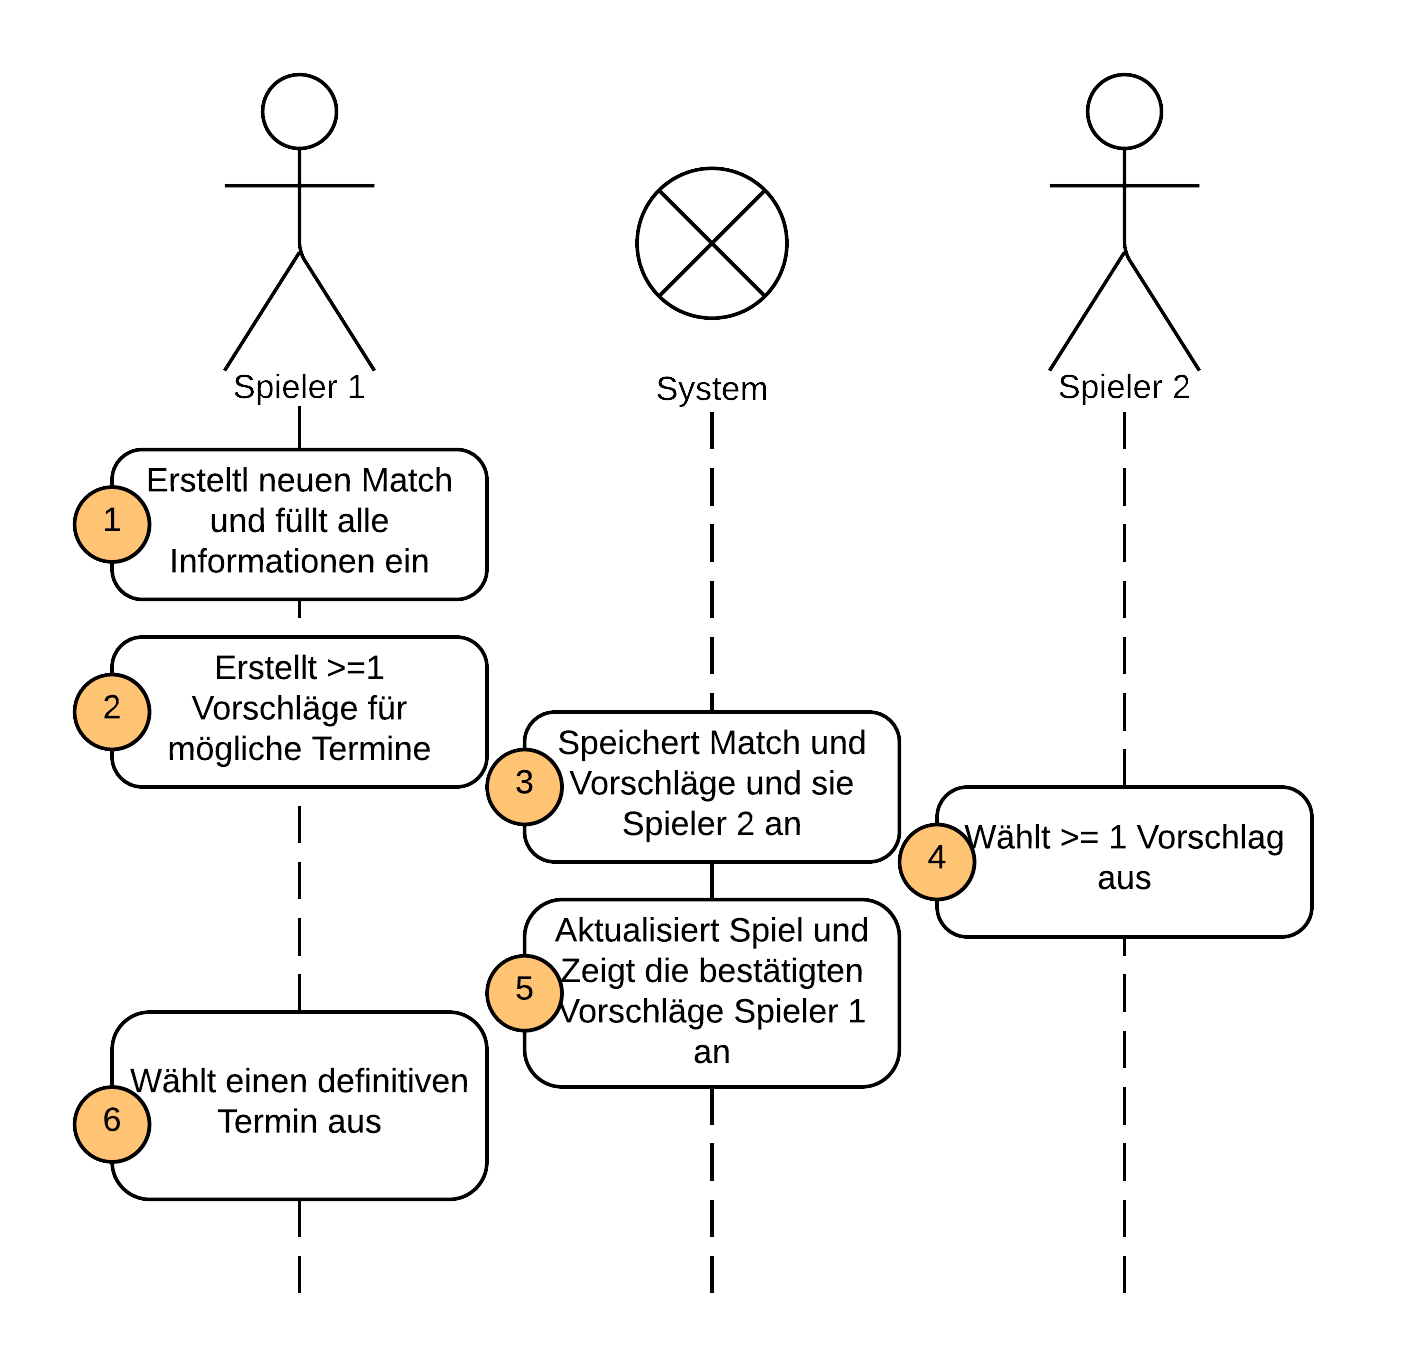
\includegraphics[width=0.7\textwidth]{Graphics/SEQSUC2.png}
		\tabularnewline
		\tabucline[2pt]{-}
		\textcolor{white}{\textbf{\cellcolor{airforceblue}Alternative Sequenzen}} & \cellcolor{testblau}
		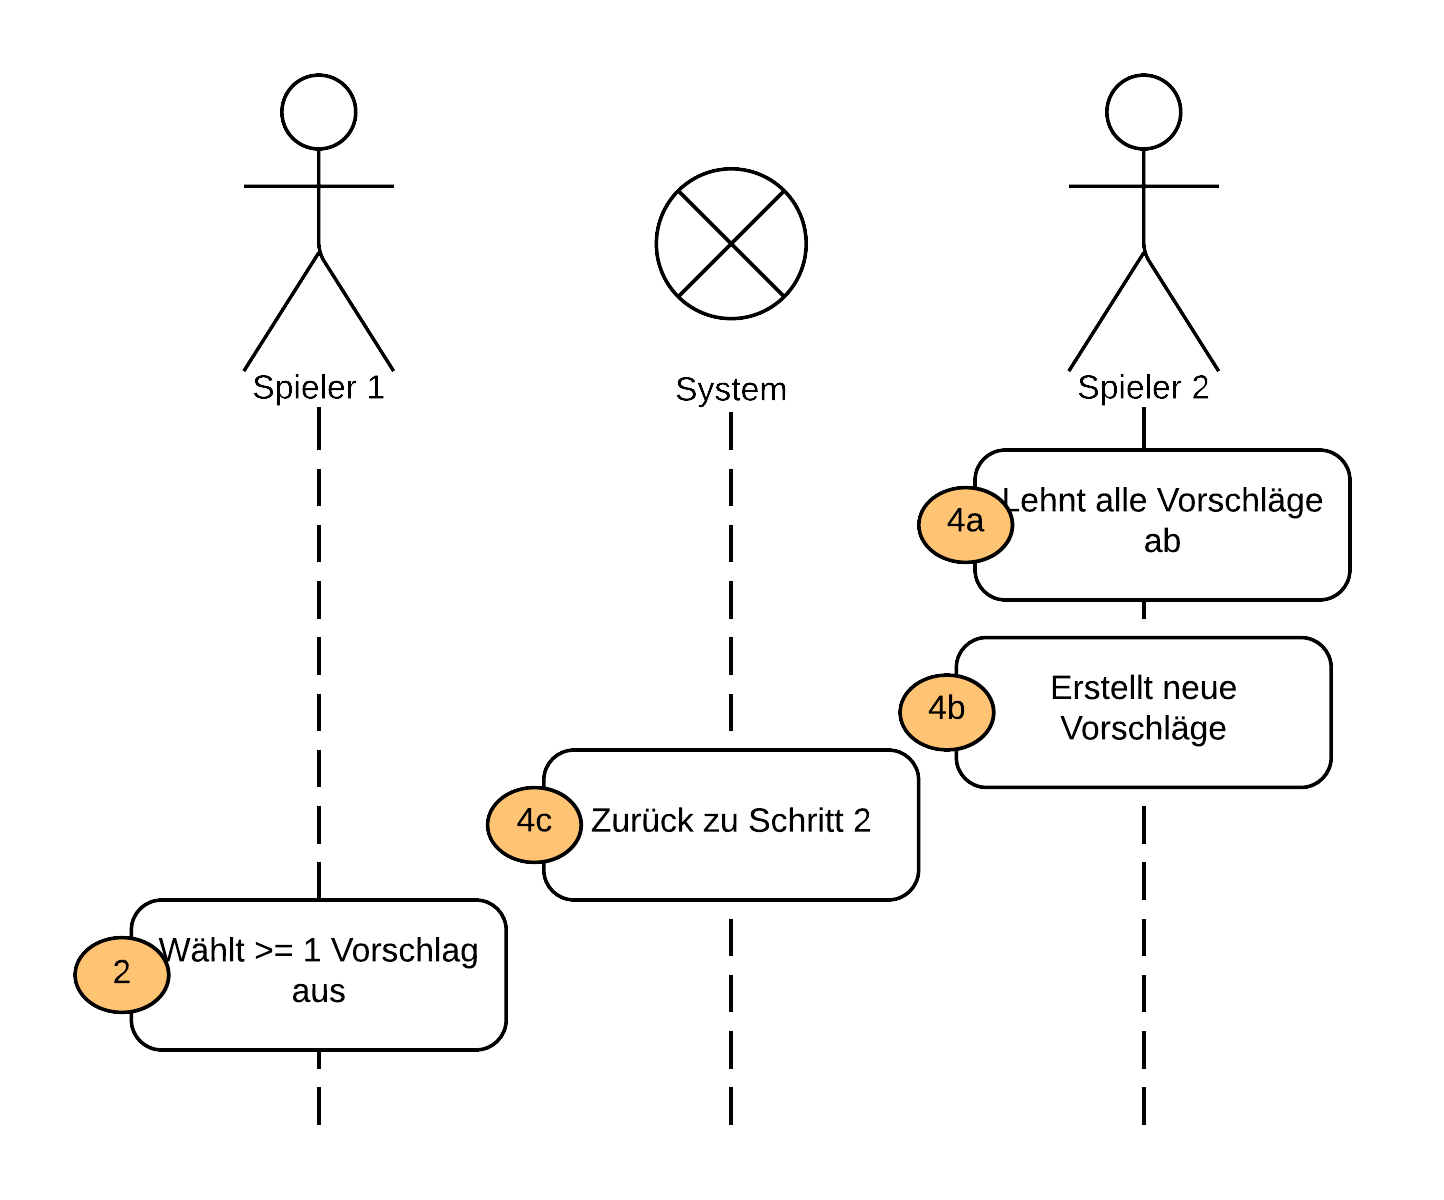
\includegraphics[width=0.7\textwidth]{Graphics/SEQA1UC2.png}
		\tabularnewline
		\tabucline[2pt]{-}
				
				
\end{longtabu}
			
\end{center}



\FloatBarrier
\newpage

\subsubsection{UC 4.1 - Liga erstellen}
\begin{center}
	
	
	\tabulinesep = 1mm
	\begin{longtabu} to \linewidth [m]{|[2pt]p{3cm}|[2pt]X[1, m , l]|[2pt]}
		\arrayrulecolor{white}
		
		\tabucline[2pt]{-}
		\textcolor{white}{\textbf{\cellcolor{airforceblue}UC4.1}}  &   
		\textcolor{white}{\textbf{\cellcolor{airforceblue}Liga erstellen }}
		\tabularnewline
		\tabucline[2pt]{-}
		\textcolor{white}{\textbf{\cellcolor{airforceblue}Beschreibung}} &  
		\cellcolor{testblau}{Jeder Spieler kann eine Liga erstellen. Diese Liga generiert eine Rangliste. Der Spieler kann anschliessend andere Spieler in die Liege einladen oder die Spieler treten der Liga bei }
		\tabularnewline
		\tabucline[2pt]{-}
		\textcolor{white}{\textbf{\cellcolor{airforceblue}Diagramm}} & 	\cellcolor{testblau}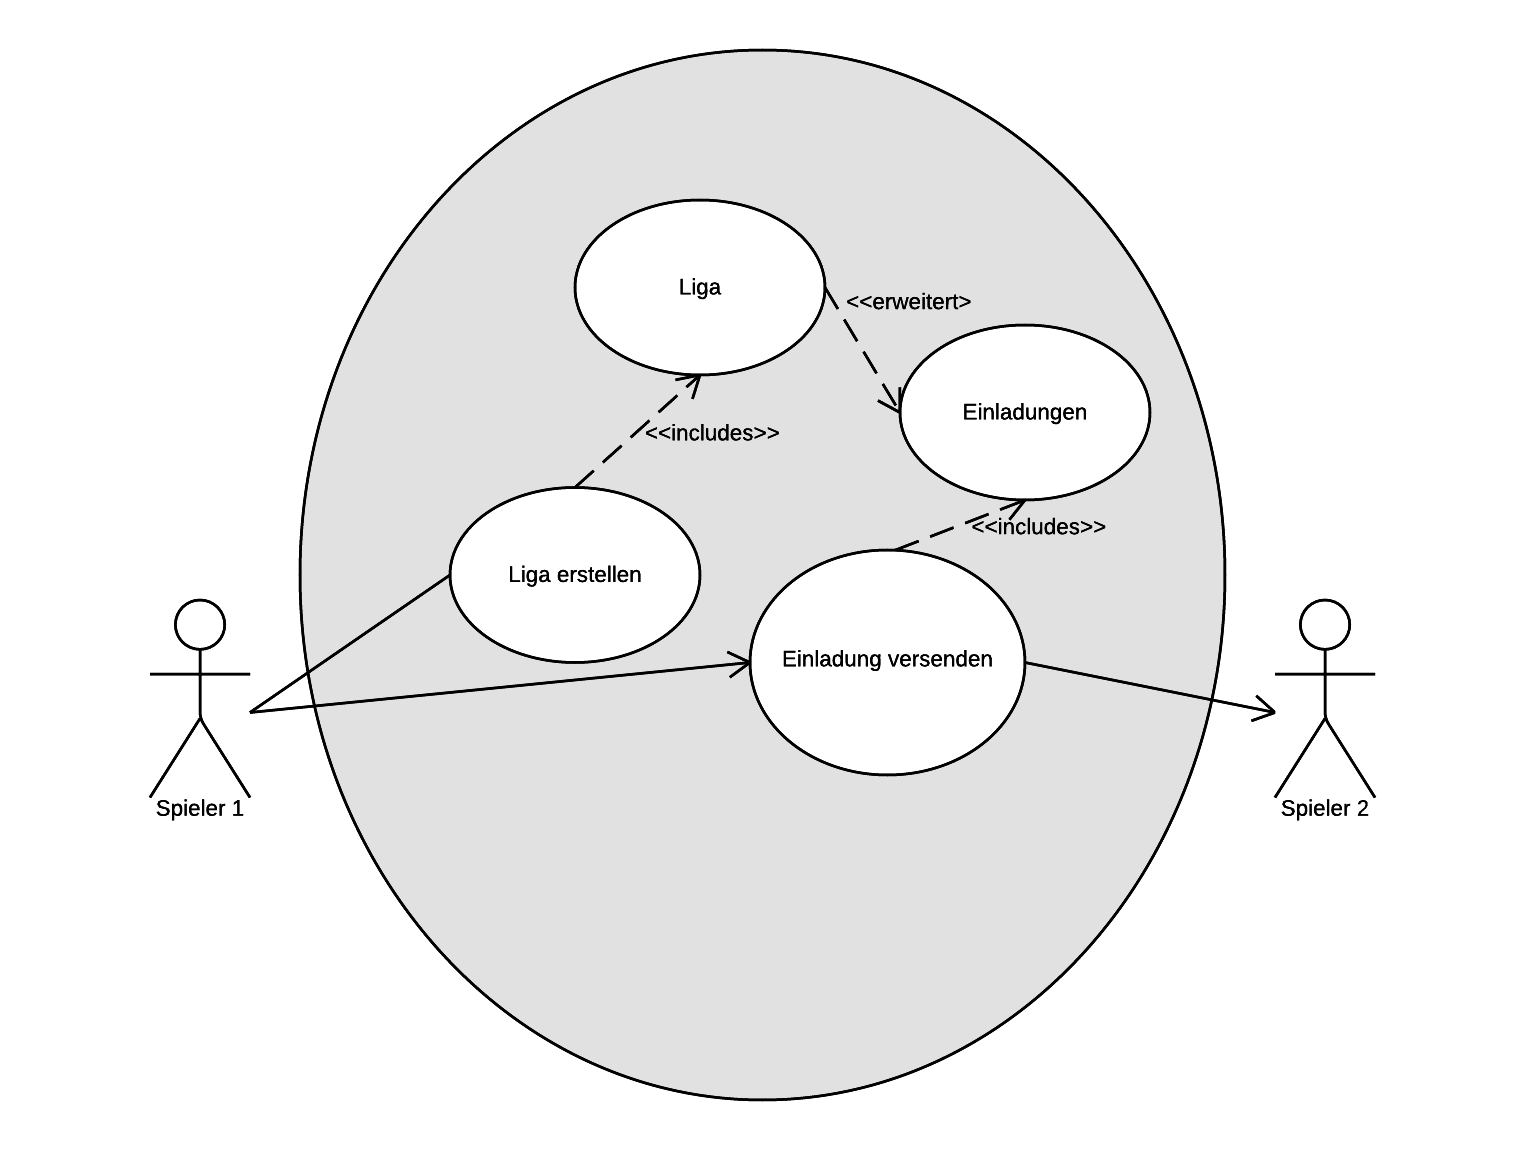
\includegraphics[width=0.8\textwidth]{Graphics/UC4_1.png}
		\tabularnewline
		\tabucline[2pt]{-}
		\textcolor{white}{\textbf{\cellcolor{airforceblue}Version}} &
		\cellcolor{testblau} 1.0
		\tabularnewline
		\tabucline[2pt]{-}
		\textcolor{white}{\textbf{\cellcolor{airforceblue}Vorbedingung}} &
		\cellcolor{testblau} 
		\begin{tabular}[x]{@{}l@{}}
			UC0 - Anmeldung an das System
		\end{tabular}
		\tabularnewline
		\tabucline[2pt]{-}
		\textcolor{white}{\textbf{\cellcolor{airforceblue}Anforderungen}} &
		\cellcolor{testblau}
		\begin{tabular}[x]{@{}l@{}}
		REQ4.01 - Liga erstellen \\
		REQ4.02 - Spieler k�nnen sich in Liga eintragen
			
		\end{tabular}
		\tabularnewline
		\tabucline[2pt]{-}
		\textcolor{white}{\textbf{\cellcolor{airforceblue}Testf�lle}} &
		\cellcolor{testblau}	
		\begin{tabular}[x]{@{}l@{}}
			Test4.1: TBD\\
			Test4.2: TBD
		\end{tabular}  
		\tabularnewline
		\tabucline[2pt]{-}
		\textcolor{white}{\textbf{\cellcolor{airforceblue}
				\begin{tabular}[x]{@{}l@{}}
					Standard\\
					Sequenz
				\end{tabular}}} & 	\cellcolor{testblau}	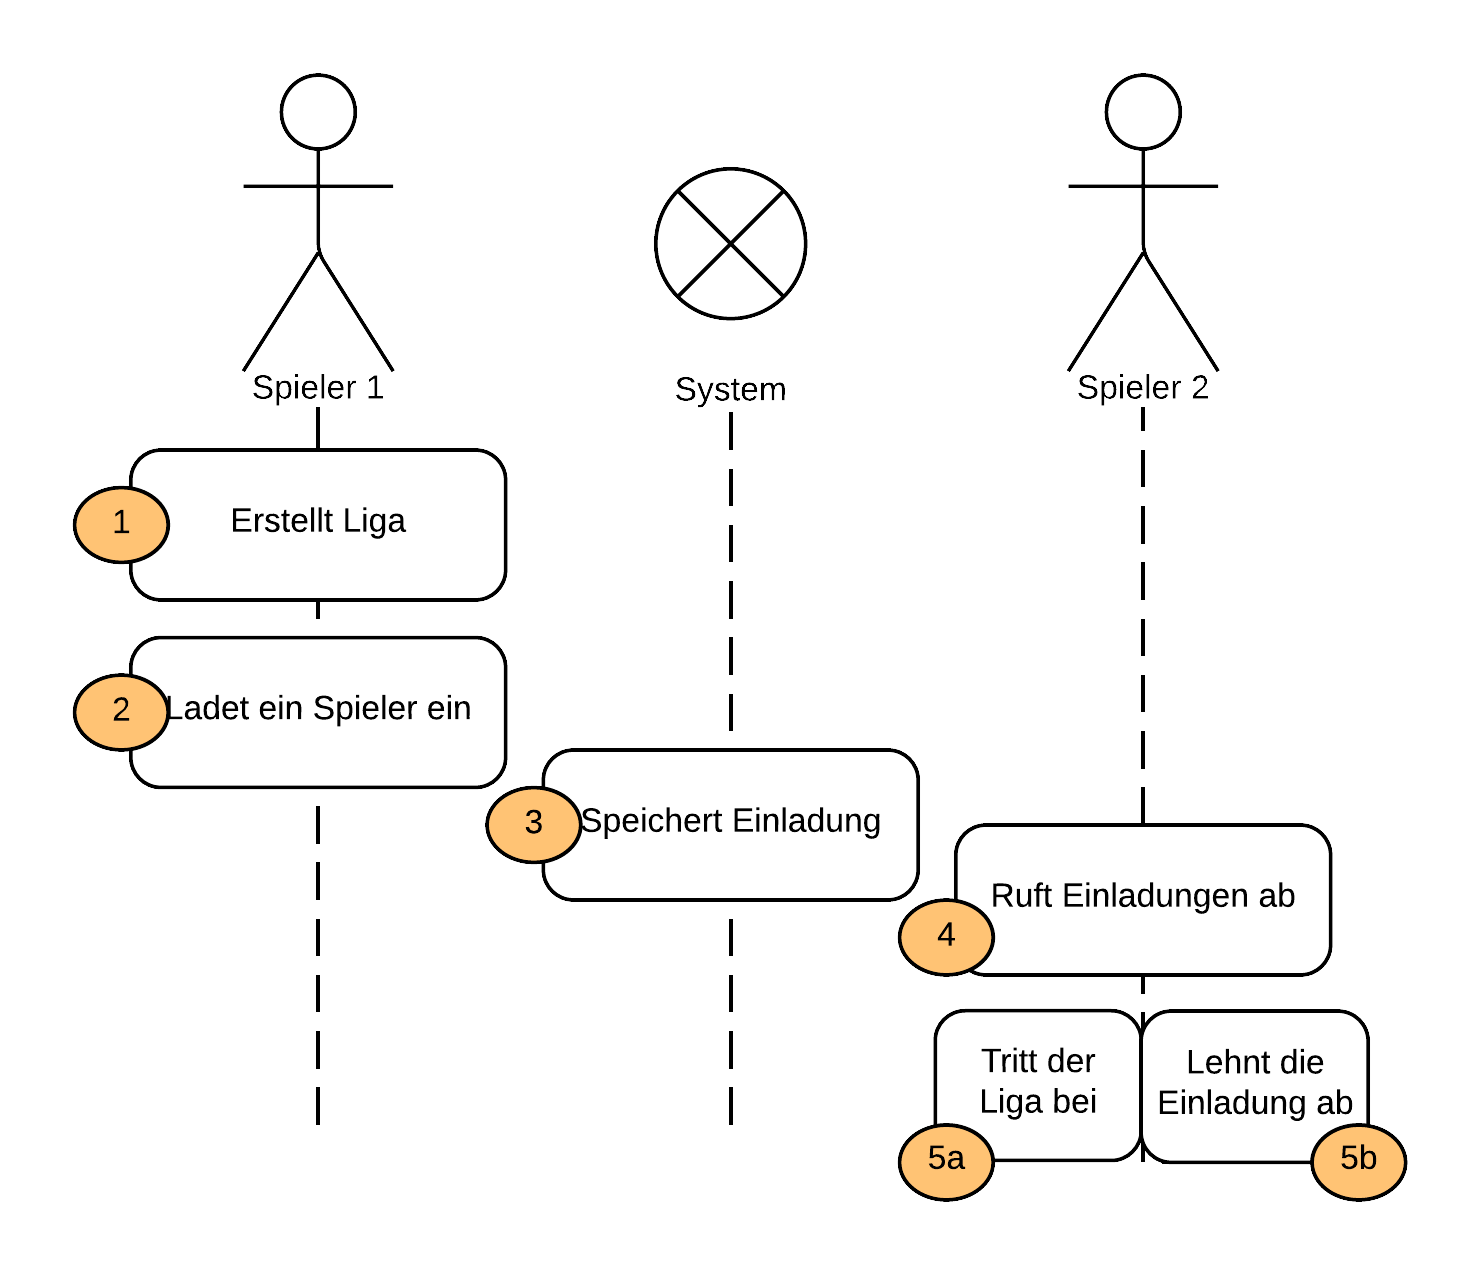
\includegraphics[width=0.7\textwidth]{Graphics/SEQSUC4_1.png}
				\tabularnewline
				\tabucline[2pt]{-}
				
				
			\end{longtabu}
			
		\end{center}

\FloatBarrier
\newpage
\subsubsection{UC 4.2 -Rangliste durch Spiele aktualisieren}

	\begin{center}
	
	\tabulinesep = 1mm
	\begin{longtabu} to \linewidth [m]{|[2pt]p{3cm}|[2pt]X[1, m , l]|[2pt]}
		\arrayrulecolor{white}
		
		\tabucline[2pt]{-}
		\textcolor{white}{\textbf{\cellcolor{airforceblue}UC4.2}}  &   
		\textcolor{white}{\textbf{\cellcolor{airforceblue}Rangliste durch Spiele aktualisieren}}
		\tabularnewline
		\tabucline[2pt]{-}
		\textcolor{white}{\textbf{\cellcolor{airforceblue}Beschreibung}} &  
		\cellcolor{testblau}{Nachdem ein Spiel gespielt ist, k�nnen beide Spieler ihre Scores eintragen. Stimmt diese �berein oder best�tigt ein Spieler der eingetragene Score des anderen Spielers, wird dieser zur Rangliste hinzugerechnet. }
		\tabularnewline
		\tabucline[2pt]{-}
		\textcolor{white}{\textbf{\cellcolor{airforceblue}Diagramm}} & 	\cellcolor{testblau}		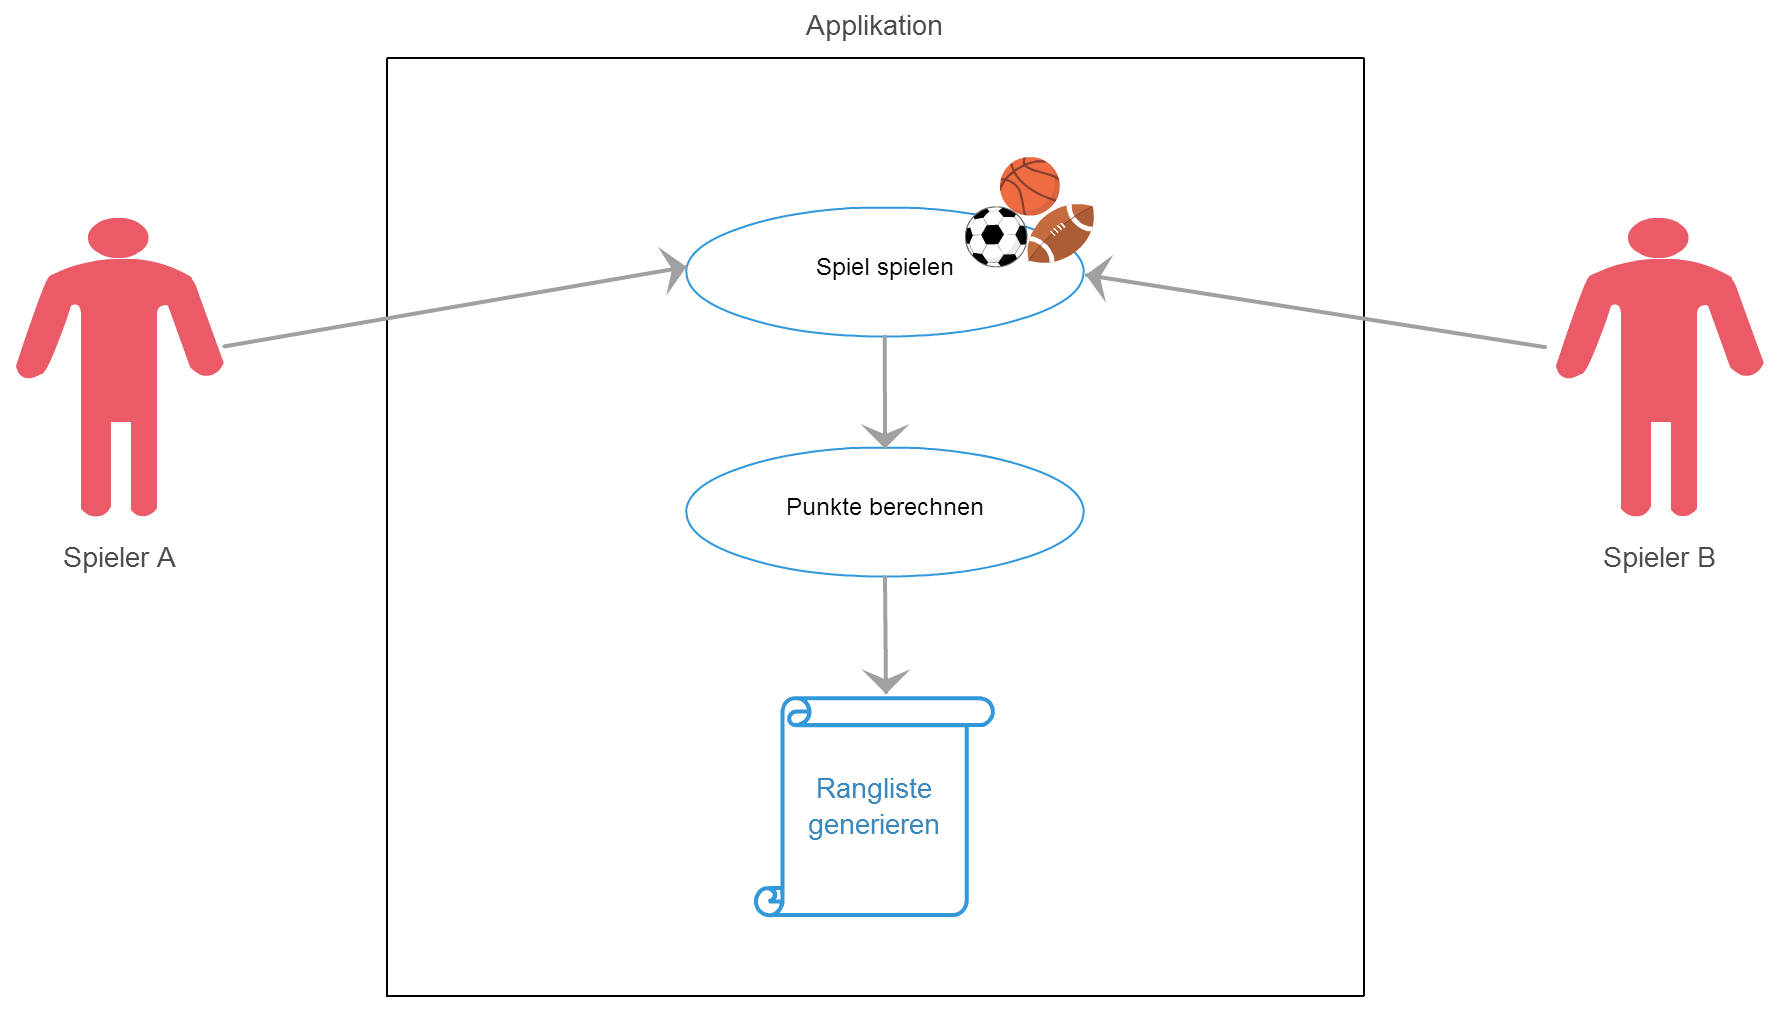
\includegraphics[width=0.7\textwidth]{Graphics/UC4_2.png}
		\tabularnewline
		\tabucline[2pt]{-}
		\textcolor{white}{\textbf{\cellcolor{airforceblue}Version}} &
		\cellcolor{testblau} 1.0
		\tabularnewline
		\tabucline[2pt]{-}
		\textcolor{white}{\textbf{\cellcolor{airforceblue}Vorbedingung}} &
		\cellcolor{testblau} UC4.1 - Liga erstellen
		\tabularnewline
		\tabucline[2pt]{-}
		\textcolor{white}{\textbf{\cellcolor{airforceblue}Anforderungen}} &
		\cellcolor{testblau}REQ4.03 - Rangliste der Liga durch Spiele
		aktualisieren 	\tabularnewline
	\tabucline[2pt]{-}
	\textcolor{white}{\textbf{\cellcolor{airforceblue}Testf�lle}} &
	\cellcolor{testblau} Test1.1: Test \\
	\cellcolor{airforceblue}&\cellcolor{testblau}Test 1.2: Test2
	\tabularnewline
	\tabucline[2pt]{-}
	\textcolor{white}{\textbf{\cellcolor{airforceblue}Szenarien}} & 	\cellcolor{testblau}		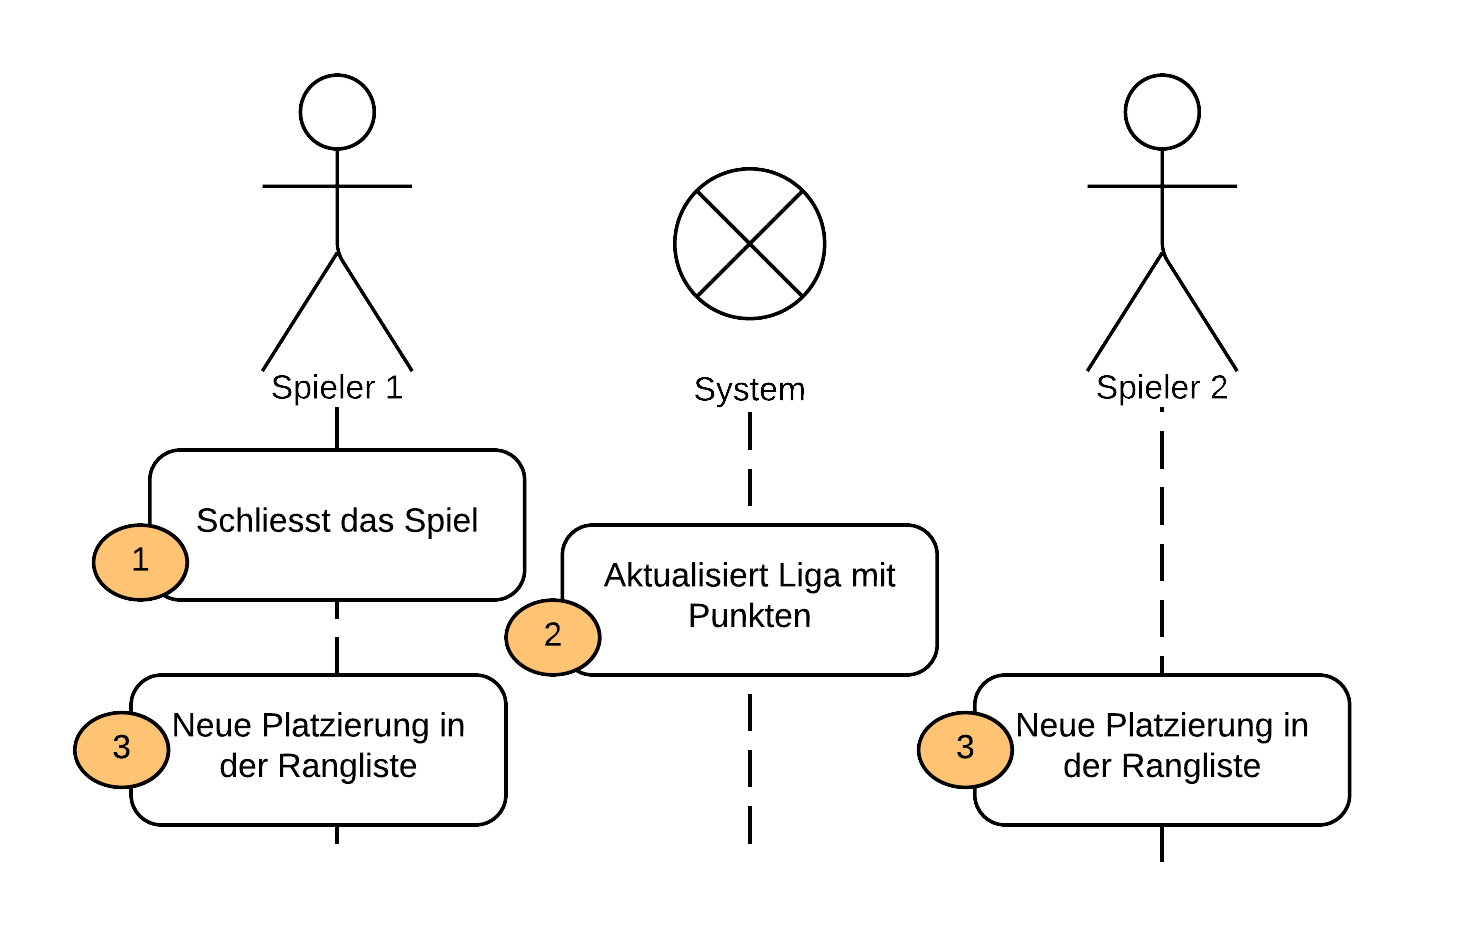
\includegraphics[width=0.7\textwidth]{Graphics/SEQSUC4_2.png}
	\tabularnewline
	\tabucline[2pt]{-}
	
	
	\end{longtabu}
\end{center}


\FloatBarrier
\newpage
\subsubsection{UC 4.3 - Spiele automatisch anfordern}
	\begin{center}
		
		\tabulinesep = 1mm
		\begin{longtabu} to \linewidth [m]{|[2pt]p{3cm}|[2pt]X[1, m , l]|[2pt]}
			\arrayrulecolor{white}
			
			\tabucline[2pt]{-}
			\textcolor{white}{\textbf{\cellcolor{airforceblue}UC4.3}}  &   
			\textcolor{white}{\textbf{\cellcolor{airforceblue}Spiele automatisch anfordern}}
			\tabularnewline
			\tabucline[2pt]{-}
			\textcolor{white}{\textbf{\cellcolor{airforceblue}Beschreibung}} &  
			\cellcolor{testblau}{Bei der Erstellung der Liga kann einen Algorithmus zur automatischen Spielvereinbarung ausgew�hlt werden. Dieser Algorithmus schl�gt jedem Spieler nach der definierten Regelm�ssigkeit Terminvorschl�ge vor und stellt so sicher, das alle Spieler regelm�ssig gegen alle andere Spieler spielen. Die Spieler k�nnen sich auf einen der vorgeschlagenen Termine - oder ein anderer individuell vorgeschlagener Termin festlegen. }
			\tabularnewline
			\tabucline[2pt]{-}
			\textcolor{white}{\textbf{\cellcolor{airforceblue}Diagramm}} & 	\cellcolor{testblau}		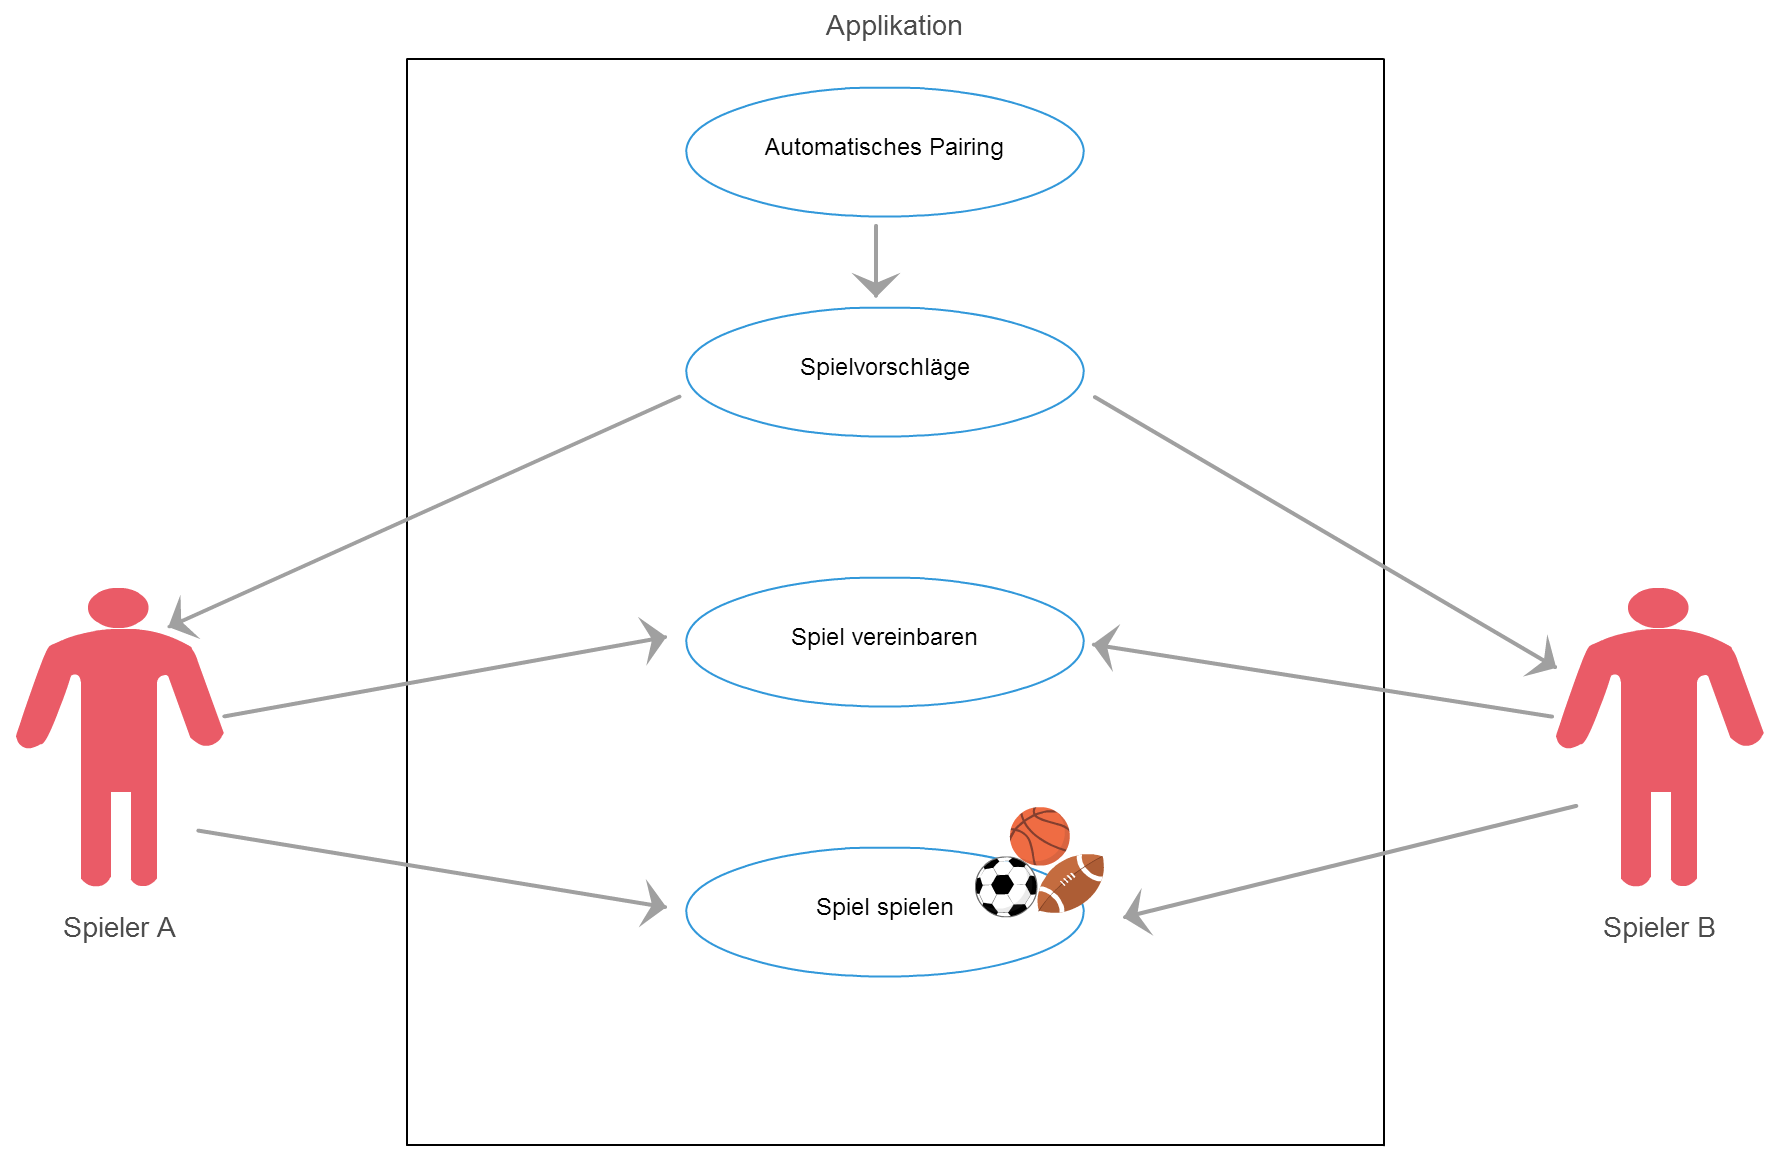
\includegraphics[width=0.7\textwidth]{Graphics/UC4_3.png}
			\tabularnewline
			\tabucline[2pt]{-}
			\textcolor{white}{\textbf{\cellcolor{airforceblue}Version}} &
			\cellcolor{testblau} 1.0
			\tabularnewline
			\tabucline[2pt]{-}
			\textcolor{white}{\textbf{\cellcolor{airforceblue}Vorbedingung}} &
			\cellcolor{testblau} UC4.1 - Liga erstellen
			\tabularnewline
			\tabucline[2pt]{-}
			\textcolor{white}{\textbf{\cellcolor{airforceblue}Anforderungen}} &
			\cellcolor{testblau}REQ4.04 - Erstellen eines automatischen Spiels 
			\tabularnewline
			\tabucline[2pt]{-}
			\textcolor{white}{\textbf{\cellcolor{airforceblue}Testf�lle}} &
			\cellcolor{testblau} Test1.1: Test \\
			\cellcolor{airforceblue}&\cellcolor{testblau}Test 1.2: Test2
			\tabularnewline
			\tabucline[2pt]{-}
			\textcolor{white}{\textbf{\cellcolor{airforceblue}Szenarien}} & 	\cellcolor{testblau}		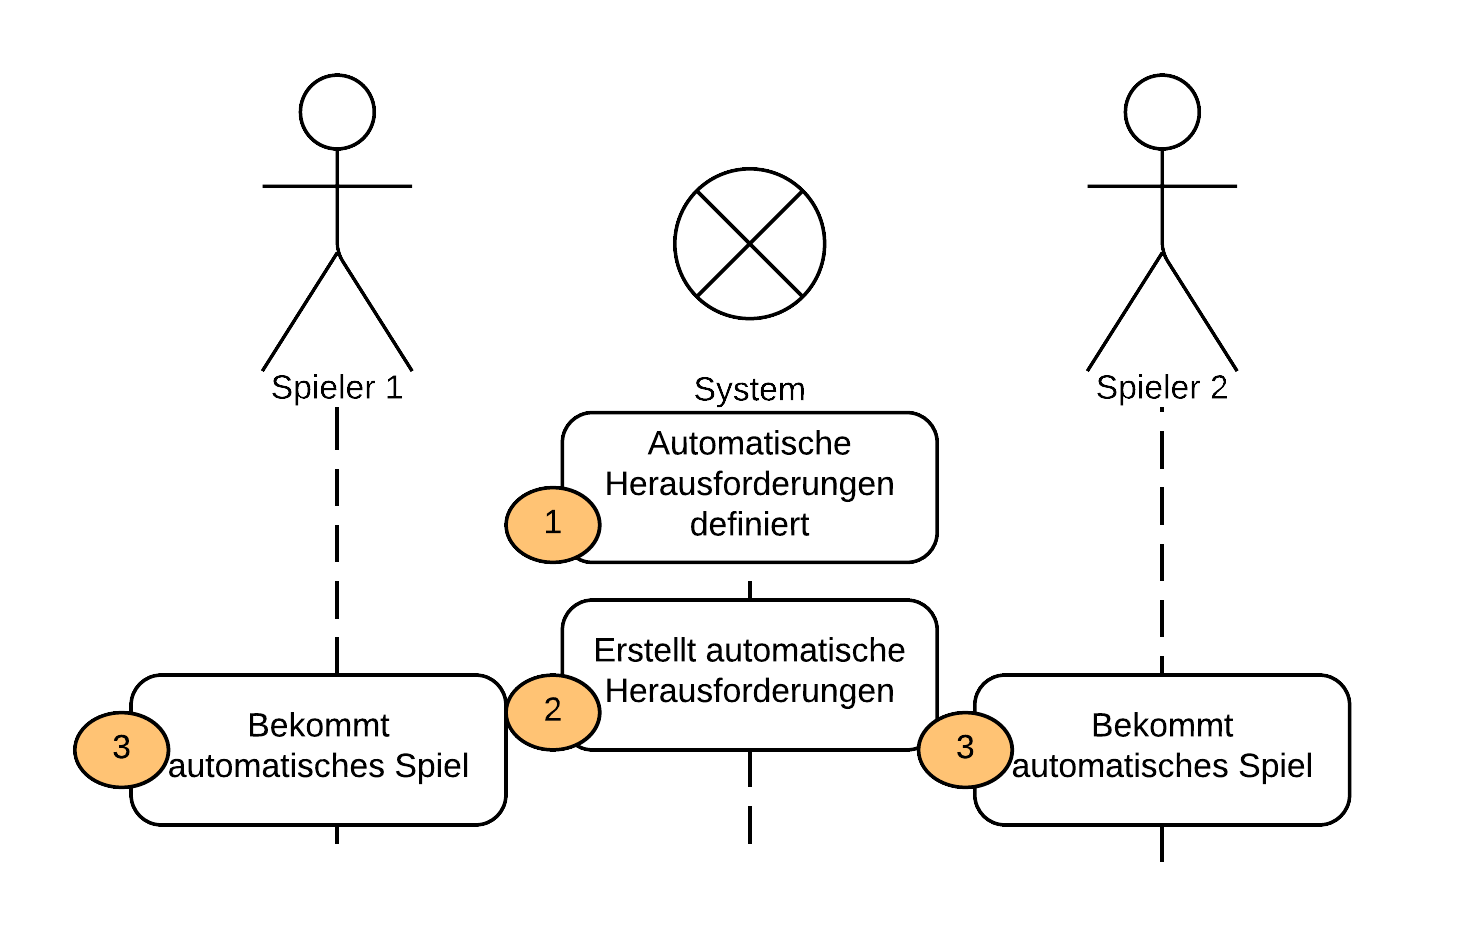
\includegraphics[width=0.7\textwidth]{Graphics/SEQSUC4_3.png}
			\tabularnewline
			\tabucline[2pt]{-}
			
			
		\end{longtabu}
	\end{center}




	
		\FloatBarrier



\subsection{Anforderungen}
Folgende Anforderungen resultieren aus den Use Cases und sind kategorisiert in funktionale- sowie nicht funktionale Anforderungen. Zus�tzlich werden die Anforderungen bewertet mit den Attributen Notwendigkeit und Kritikalit�t.

Folgende Kategorien k�nnen f�r Notwendigkeit vergeben werden:
\begin{itemize}
	\itemsep-0.4em
	\item Essential - Anforderung in der Aufgabenstellung enthalten und/oder Notwendig f�r den PoC
	\item Conditional - Anforderung verbessert die App massiv und w�rde L�sung erweitern. Ein nicht Erf�llen der Anforderung macht die L�sung jedoch nicht inakzeptabel und kann in zuk�nftigen Releases umgesetzt werden
	\item Optional - K�nnen umgesetzt werden, m�ssen jedoch nicht. Je nach Feedback von zuk�nftigen Kunden k�nnten optionale Anforderungen in Zukunft ber�cksichtigt werden
\end{itemize}

F�r Kritikalit�t gibt es folgende Kategorien:
\begin{itemize}
	\itemsep -0.4em
	\item High - Anforderung ist Basis von anderen essential Anforderungen und muss schnell erstellt werden
	\item Medium - Anforderung sollte innerhalb des POC implementiert werden um Benutzerf�lle vollst�ndig abzudecken
	\item Low - Anforderung kann in zuk�nftigen Releases umgesetzt werden
\end{itemize}

Die Anforderung in diesem Abschnitt werden  in User Stories �bertragen in das Tool Yodiz: \url{https://app.yodiz.com/plan/pages/task-board.vz?cid=14274&pid=1&iid=1}


\subsubsection{Funktionale Anforderungen}
Funktionale Anforderungen definierten spezifische, aus den Anwendungsf�llen ben�tigte, Funktionalit�ten der Applikation. 
\begin{center}
	\tabulinesep = 1mm
	\begin{longtabu} to \linewidth [m]{X[1, m , l]|[2pt]p{2.95cm}|[2pt]p{2.5cm}|[2pt]}
		\arrayrulecolor{white}
		
		\tabucline[2pt]{-}
		\textcolor{white}{\textbf{\cellcolor{airforceblue}Anforderung}}  &  
		\textcolor{white}{\textbf{\cellcolor{airforceblue}Notwendigkeit}}&
		\textcolor{white}{\textbf{\cellcolor{airforceblue}Kritikalit�t}}
		\tabularnewline
			\tabucline[2pt]{-}
		\multicolumn{3}{l}{\cellcolor{bluegray}  Kategorie Bedienbarkeit  }
		\tabularnewline
		\cellcolor{testblau}  REQ0.01 - Anmeldung an das System  &
		\cellcolor{testblau}  Essential &
		\cellcolor{testblau}High
		\tabularnewline
		\cellcolor{testblau}  REQ0.02 - Registrierung eines Users mit dem System  &
		\cellcolor{testblau}  Essential &
		\cellcolor{testblau}High
		\tabularnewline
		\cellcolor{testblau}  REQ0.03 - Authentisierung �ber OAuth  &
		\cellcolor{testblau}  Conditional &
		\cellcolor{testblau}High
		\tabularnewline
		\tabucline[2pt]{-}
		\multicolumn{3}{l}{\cellcolor{bluegray}  Kategorie User  }
		\tabularnewline
		\cellcolor{testblau}  REQ1.01 - Zuteilung von User zu Racketsportzentren  &
		\cellcolor{testblau}Essential &
		\cellcolor{testblau}High
		\tabularnewline
		\cellcolor{testblau}  REQ1.02 - Details zu Spielern  &
		\cellcolor{testblau}Essential &
		\cellcolor{testblau}High
		\tabularnewline
		\cellcolor{testblau}  REQ1.03 - Friend System  &
		\cellcolor{testblau}Conditional &
		\cellcolor{testblau}Medium
		\tabularnewline
		\tabucline[2pt]{-}
		\multicolumn{3}{l}{\cellcolor{bluegray}  Kategorie Spiele  }
		\tabularnewline
		\cellcolor{testblau}  REQ2.01 - Spiel erstellen  &
		\cellcolor{testblau}Essential &
		\cellcolor{testblau}High
		\tabularnewline
		\cellcolor{testblau}  REQ2.02 - Spiel Terminvorschl�ge erstellen  &
		\cellcolor{testblau}Essential &
		\cellcolor{testblau}High
		\tabularnewline
		\cellcolor{testblau}  REQ2.03 - Spiel Terminvorschl�ge annehmen und ablehnen  &
		\cellcolor{testblau}Essential &
		\cellcolor{testblau}High
		\tabularnewline
		\cellcolor{testblau}  REQ2.04 - Wiederkehrende Spiele erstellen  &
		\cellcolor{testblau}Essential &
		\cellcolor{testblau}High
		\tabularnewline
		\cellcolor{testblau}  REQ2.05 -  Broadcast Spiele erstellen  &
		\cellcolor{testblau}Conditional &
		\cellcolor{testblau}Medium
		\tabularnewline
		\cellcolor{testblau}REQ2.06 -  Privatsph�reeinstellungen ber�cksichtigen  &
		\cellcolor{testblau}Optional &
		\cellcolor{testblau}Low
		\tabularnewline
		\cellcolor{testblau}REQ2.07 -  Ergebnissedes Spiels Eintragen  &
		\cellcolor{testblau}Essential &
		\cellcolor{testblau}High
		\tabularnewline
		\cellcolor{testblau}REQ2.08 -  Best�tigung des Spiels eintragen &
		\cellcolor{testblau}Essential &
		\cellcolor{testblau}High
		\tabularnewline
		\tabucline[2pt]{-}
		\multicolumn{3}{l}{\cellcolor{bluegray} Kategorie Courts  }
		\tabularnewline
		\cellcolor{testblau}REQ3.01 -  Courts erstellen &
		\cellcolor{testblau}Essential &
		\cellcolor{testblau}High
		\tabularnewline
		\cellcolor{testblau}REQ3.02 -  Spieler k�nnen sich in Courts eintragen &
		\cellcolor{testblau}Essential &
		\cellcolor{testblau}High
		\tabularnewline
		\tabucline[2pt]{-}
		\multicolumn{3}{l}{\cellcolor{bluegray} Kategorie Liga  }
		\tabularnewline		
		\cellcolor{testblau}REQ4.01 -  Liga erstellen &
		\cellcolor{testblau}Essential &
		\cellcolor{testblau}High
		\tabularnewline
		\cellcolor{testblau}REQ4.02 -  Spieler k�nnen sich in Liga eintragen &
		\cellcolor{testblau}Essential &
		\cellcolor{testblau}High
		\tabularnewline
		\cellcolor{testblau}REQ4.03 - Rangliste der Liga durch Spiele aktualisieren &
		\cellcolor{testblau}Essential &
		\cellcolor{testblau}High
		\tabularnewline
		\cellcolor{testblau}REQ4.04 -  Erstellen eines automatischen Spiels&
		\cellcolor{testblau}Essential &
		\cellcolor{testblau}High
		\tabularnewline
	\end{longtabu}\end{center}
\subsubsection{Nicht funktionale Anforderungen}
Die nicht funktionalen Anforderungen definieren Eigenschaften der Applikation, welche erf�llt werden sollten, jedoch nicht f�r den User ersichtlich sind. Diese Anforderungen sind wichtig sobald eine solche Applikation in einen produktiven Status �bergeht. Im Moment ist die Applikation in einem PoC Status geplant, deshalb sind viele nicht funktionale Anforderungen optional.

\begin{center}
	\tabulinesep = 1mm
	\begin{longtabu} to \linewidth [m]{X[1, m , l]|[2pt]p{2.95cm}|[2pt]p{2.5cm}|[2pt]}
		\arrayrulecolor{white}
		
		\tabucline[2pt]{-}
		\textcolor{white}{\textbf{\cellcolor{airforceblue}Anforderung}}  &  
		\textcolor{white}{\textbf{\cellcolor{airforceblue}Notwendigkeit}}&
		\textcolor{white}{\textbf{\cellcolor{airforceblue}Kritikalit�t}}
		\tabularnewline
		\tabucline[2pt]{-}
		\multicolumn{3}{l}{\cellcolor{bluegray}  Qualit�tsmerkmal:  Funktionalit�t }
		\tabularnewline
		\cellcolor{testblau}  NREQ0.01 - Sicherheit &
		\cellcolor{testblau}  Conditional &
		\cellcolor{testblau}High
		\tabularnewline
		\tabucline[2pt]{-}
		\multicolumn{3}{l}{\cellcolor{bluegray}  Qualit�tsmerkmal:  Zuverl�ssigkeit  }
		\tabularnewline
		\cellcolor{testblau}  NREQ1.01 - Fehlertoleranz  &
		\cellcolor{testblau}Conditional &
		\cellcolor{testblau}High
		\tabularnewline		
		\cellcolor{testblau}  NREQ1.02 - Wiederherstellbarkeit  &
		\cellcolor{testblau}Essential &
		\cellcolor{testblau}High
		\tabularnewline	
		\tabucline[2pt]{-}
		\multicolumn{3}{l}{\cellcolor{bluegray}  Qualit�tsmerkmal:  Benutzbarkeit  }
		\tabularnewline
		\cellcolor{testblau}  NREQ2.01 - Verst�ndlichkeit  &
		\cellcolor{testblau}Optional &
		\cellcolor{testblau}Medium
		\tabularnewline		
		\cellcolor{testblau}  NREQ2.02 - Bedienbarkeit  &
		\cellcolor{testblau}Conditional &
		\cellcolor{testblau}High
		\tabularnewline
		\tabucline[2pt]{-}
		\multicolumn{3}{l}{\cellcolor{bluegray}  Qualit�tsmerkmal:  Effizienz  }
		\tabularnewline
		\cellcolor{testblau}  NREQ3.01 - Effizient in Programmierung  &
		\cellcolor{testblau} Essential &
		\cellcolor{testblau} High
		\tabularnewline		
		\cellcolor{testblau}  NREQ3.02 - Effizient in Installation  &
		\cellcolor{testblau} Essential &
		\cellcolor{testblau}High
		\tabularnewline
		\tabucline[2pt]{-}
		\multicolumn{3}{l}{\cellcolor{bluegray}  Qualit�tsmerkmal:  Wartbarkeit  }
		\tabularnewline
		\cellcolor{testblau}  NREQ4.01 - Einfach erweiterbar/�nderbar &
		\cellcolor{testblau} Essential &
		\cellcolor{testblau} High
		\tabularnewline		
		\cellcolor{testblau}  NREQ4.02 - Stabilit�t  &
		\cellcolor{testblau} Optional &
		\cellcolor{testblau} High
		\tabularnewline
				\cellcolor{testblau}  NREQ4.03 - Testbarkeit  &
				\cellcolor{testblau} Essential &
				\cellcolor{testblau} High
				\tabularnewline
		\cellcolor{testblau}  NREQ4.04 - Analysierbarkeit    &
		\cellcolor{testblau} Optional &
		\cellcolor{testblau} High
		\tabularnewline		
		
	
	\end{longtabu}\end{center}
	
	Diese nicht funktionalen Anforderungen m�ssen immer im PoC angeschaut werden. Optionale Anforderungen k�nnen f�r einen produktiven Einsatz neu als essential ne kategorisiert werden.
	
	

% !TeX spellcheck = de_DE
\chapter{Konzeption}
\begin{figure}[ht]
	\centering
	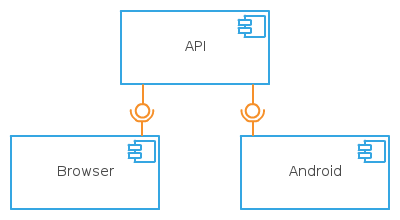
\includegraphics[width=0.5\textwidth]{Graphics/KonzeptApp.png}
	\caption{Grobkonzept f�r Applikation}
	\label{fig1}
\end{figure}
\FloatBarrier
Die Applikation besteht aus drei Teilen. Einem Webserver, der eine API und statische Clientfiles zur Verf�gung stellt, der Client im Browser, welcher die API konsumiert sowie eine Android Applikation welche die Website l�dt. 
 
\section{Technologiestack}
Wie in dem Grobkonzept beschrieben, wird f�r die Applikation einen Technologiestack gebraucht, welcher  eine skalierbare API sowie eine gute Integration der API mit einer Browser Frontend Anwendung bietet. Folgende Anforderungen werden an den Technologiestack gestellt:
\begin{itemize}
	\itemsep-0.5em
	\item Skalierbare REST API
	\item Einfacher und schneller Umgang mit AJAX
	\item Gute Integration zwischen API und HTML/JS Client
	\item Responsive Design, Integration mit OAUTH f�r 3rd Party Authentisierung
	\item Persistance Layer (Datenbankunterst�tzung)
\end{itemize} 

\subsection{MVC Frameworks}
Komplexe Applikationen werden vorzugsweise mit MVC Frameworks erstellt. �ber MVC APIs sind Routing,  Logik sowie Pr�sentationsschicht gut voneinander Abstrahiert. Es ist gut m�glich, f�r Views mit verschiedenen Daten �ber ein Model zu versehen, oder auch ein Logisches Routing f�r eine API zu entwickeln. Folgende Graphik zeigt ein MVC Konzept. Der Client sendet einen Request zu dem Server und wird vom Routing zur Logik im System weitergeleitet. Die Logik findet das richtige Model sowie die dazugeh�rige View.  Die View wird mit dem Model gerendert und es entsteht eine Antwort, welche dem Client zur�ckgesendet wird. In einer REST API ist die View JSON. Das Model wird in JSON umgewandelt und versendet. 

Folgendes Code-Beispiel - die Funktion list() -  zeigt, wie alle Courts aus dem Persistance Layer selektiert werden und per JSON zum Client gesendet werden. Dies ist ein API Endpunkt zur auflistung von Courts (http://webserver/courts). Gut zu sehen ist, dass die jsonp() Funktion als Renderer gebraucht wird anstatt eine Standard-View. 
\begin{lstlisting}
exports.list = function(req, res) { 
	Court.find().sort('-created').populate('user')
	 .exec(function(err, courts) {
		if (err) {
			return res.status(400).send({
				message: 
				 errorHandler.getErrorMessage(err)
			});
		} else {
		res.jsonp(courts);
		}
	});
};
\end{lstlisting}

Mit einem MVC Framework auf der Server-Seite kann man so gut abstrahierte und ausbauf�hige - skalierbare - APIs erstellen. Diese APIs m�ssen nun jedoch vom Client Browser verarbeitet werden k�nnen. Folgende M�glichkeiten bieten sich an:
\begin{itemize}
	\item Parallel zu der REST API werden Renderer gebaut, welche das Model mit einer View in eine - f�r den Client statische - Website rendern. Der Client verf�gt hier ausschliesslich Logik um die verschiedenen Webseiten abzurufen. 
	\item Ein Website-Skelett mit Logik wird beim ersten Aufruf an den Client verschickt. Der Client bezieht nun Daten aus der REST API und reichert die schon vorhandenen Views mit den Objekten - gesendet �ber AJAX - selber an. 
\end{itemize}
Eine parallele Implementierung zur Rest API geht entgegen dem Basis Konzept, dass alle Applikationen so gut wie m�glich von der REST API profitieren. Zus�tzlich w�rde bei einer parallelen Implementierung jeder Klick in einer Aktualisierung der Applikation resultieren. Dies ist unerw�nscht, da sich die Website nicht schnell und intuitiv anf�hlt. Man hat bei jedem Klick eine Downtime, da viel Daten �bertragen werden m�ssen, und der Browser den DOM jedes mal neu Aufbauen muss. Bei der zweiten Option wird die Website nur einmal heruntergeladen. Der DOM wird nach dem Download aufgebaut und von der Logik ver�ndert. Klicks l�sen einen viel geringeren Aufwand von Server bis Client aus und somit ist die Downtime viel kleiner. Die Applikation f�hlt sich schneller und intuitiver an. 

Wie bei dem Server, kann man auch bei der Applikation ein MVC Pattern implementieren. Ein Routing definiert, bei welchr URL welche View aufgerufen wird. Bei dem Aufruf einer View ist ein Controller hinterlegt, welcher bei der API das Model und Objekt besorgt. Die View rendert die vom Controller generierten Daten

\glqq Figure Angular JS \grqq 

Server und Client MVCs k�nnen so miteinander Kombiniert werden und es entsteht eine skalierbare und wartbare Applikationsumgebung.


\subsubsection{Server MVCs}
MVCs f�r den Server gibt es verschiedene:
\begin{itemize}
	\item Spring Framework - Java
	\item ExpressJS - JSON
	\item Rails - Ruby
\end{itemize}

\subsubsection{Client MVCs}
MVC f�r den Server sind ausschliesslich in Javascript geschrieben:
\begin{itemize}
	\item AngularJS
	\item ???
	\end{itemize}

\subsubsection{Stacks}
Eine Konfiguration des Client- sowie Server MVCs, damit beide gut miteinander Funktionieren ist zus�tzlich wichtig. In der Evaluation wird somit folgende Konfigurationen abgewogen:
\begin{itemize}
	\item Spring Framework mit AngularJS
	\item Express Framework mit AngularJS
\end{itemize}

\subsection{Spring + AngularJS}
Spring ist ein MVC Framework in Java. Man Programmiert in der J2EE Umgebung und bietet eine API zum Client. Gleichzeitig sendet man den AngularJS Stack zum Client, welcher anschliessend die API konsumiert. Als Persistance Layer k�nnen Relationale Datenbanken wie MySQL, Oracle oder Sybase verwendet werden. �ber Data Access Object wird dieser Layer angesprochen und in Models Emuliert. 

Folgende Vor- / Nachteile bring das Spring-Angular Setup mit:
\begin{itemize}
		 \itemsep-0.5em
	\item + reife Technologien, Markt erprobt
	\item + viel Know-How auf dem Markt in Java/Spring
	\item + Anbindung an Zahlreiche Persistance Layer Applikationen
	\item - Viele Daten-Transformationen (Relationale DB <-> Java Objekt <-> JSON Object)
	\item - Kompliziertes Setup
\end{itemize}

\newpage
\subsection{MEAN Stack}
Der MEAM Stack besteht aus folgender Produkten:
\begin{itemize}
		 \itemsep-0.5em
	\item M - MongoDB, der Skalierbare Persistance Layer
	\item E - ExpressJS, ein MVC um APIs zu entwickeln
	\item A - AngularJS, ein MVC auf dem Client um Sing-Page Applikationen zu erstellen, welche auf die ExpressJS API zugreifen.
	\item N - NodeJS, JavaScript Applikationsserver, welcher sehr gut skalierbar ist.
\end{itemize}

Folgende Vor- / Nachteile bring das MEAN Stack Setup mit:
\begin{itemize}
		 \itemsep-0.5em
	\item + Kleine Daten Transformationen (JSON Object wird in MongoDB gespeichert)
	 \item + Gleiche Programmiersprachen (JavaScript, HTML, CSS)
	\item + Einfaches Setup, grosse Flexibilit�ten
	\item + Innovative Technologien
	\item - Wenig Markt erprobt
\end{itemize}

\subsection{Entscheidung}
Da das Ergebnis dieser Arbeit ein Proof of Concept darstellt, und die Applikation nicht ausgereift sein wird zum Zeitpunkt der Abgabe, sowie eine produktiver Nutzen nicht das Ziel dieser Aufgabenstellung ist, will der Autor mit m�glichst innovativen, flexiblen und einfachen Technologien arbeiten. Der MEAN Stack scheint dadurch der optimale Kandidat f�r dieses Projekt.

\section{Architektur}
Die Applikation ist aufgeteilt auf einen Server, sowie auf einen Client, welcher ein Browser oder eine Android App ist. Auf dem Server sind alle Daten hinterlegt:
\begin{itemize}
	\itemsep -0.5em
	\item Gespeicherte Objekte in MongoDB
	\item Server Logik
	\item Client Daten, welche vom Browser �ber HTTP abgefragt werden
\end{itemize}

Im Anfangszustand hat der Client keine Daten. Der Client bekommt die Daten bei dem Abruf der Applikations URL �ber HTTP. Er baut nun die Logik im Browser Cache auf und startet das JavaScript Programm. Das JavaScript Programm l�dt nun die auf dem Server gespeicherten Objekte �ber HTTP AJAX Abrufe und stellt diese dar.  

Die Logik von Server wie auch Client benutzt das M(V)C Pattern. Objecte werden in Models - inklusive Business Logik -  gespeichert, der Controller beinhaltet die Applikationslogik, welche das Model sowie die View ausw�hlt. Die View rendert nun das Model in ein bestimmtes Schema (siehe Abbildung \ref{DetAppArch}). 
\begin{figure}[ht]
	\centering
	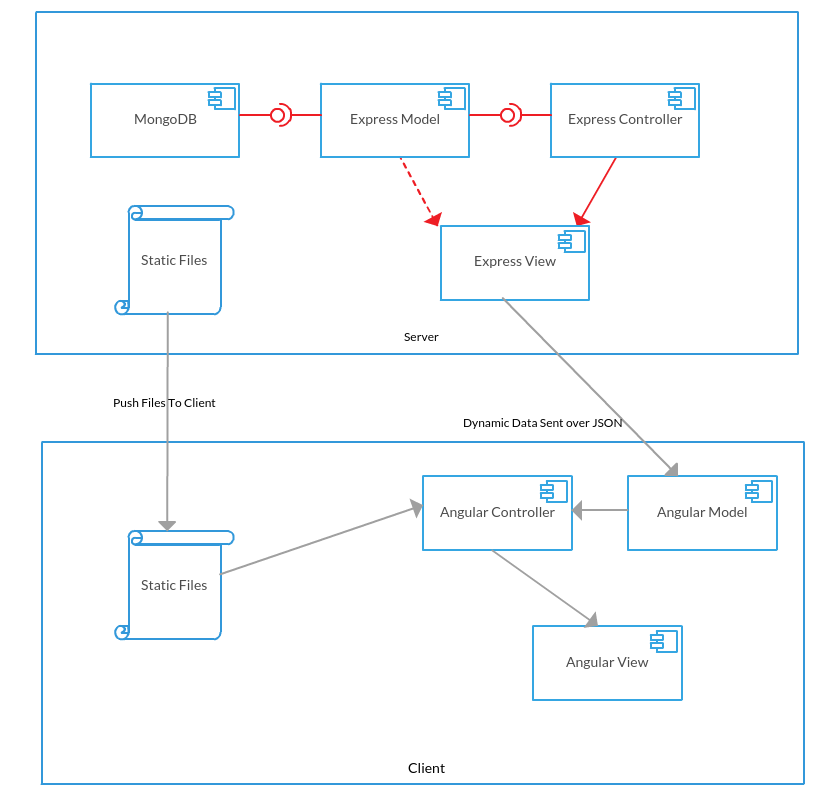
\includegraphics[width=0.9\textwidth]{Graphics/DetailAppArch.png}
	\caption{Detaillierte Applikations Architektur}
	\label{DetAppArch}
\end{figure}


\section{DB Design}
In der Applikation gibt es kein Relationales Datenbankmodel. MongoDB arbeiet mit Dokumenten, sowie Referenzen. Dokumente sind JSON-Objekte in JavasScript, welche in MongoDB als Dokument gespeichert werden. Ein Objekt ist eine Representation von Business Objekten in der Applikation.

Das User-Objekt repr�sentiert der User der Applikation. Der User hat einen Namen, einen Usernamen, ein Passwort (encrypted und salted), Berechtigungen und Freunde. Zus�tzlich werden Ihm andere Objekte zugeordnet sowie andere User (Repr�sentation als Freund).

Das Court-Objekt repr�sentiert ein Racketsportzentrum der Applikation. Dieses Objekt wird ben�tigt um den Physikalischen Austragungsort eines Spieles zu definieren. Das Objekt beinhaltet einen Namen, eine Adresse (inklusive Koordinaten f�r eine zuk�nftige Umkreissuche), was f�r Sportarten gespielt werden k�nnen und welche User in diesem Racketsportzentrum spielen wollen.

Das Match-Objekt resp�sentiert das Spiel, welches geplant, ausgetragen oder beendet ist. Das Spiel-Modell definiert zwei oder einen Spieler, einen Status, eine Sportart, ein Court, mehrere Datumvorschl�ge, maximal fixes Datum, eine Punkzahl, sowie ein Gewinner. Hinter dem Match-Objekt existiert ein relativ grosser Business-Workflow, welcher im Kapitel <<<<IMPLEMENTATION Matchmaking>>>> definiert ist. 

Das Liga-Objekt repr�sntiert eine Liga. Verschiedene Benutzer k�nnen einer Liga beitereten und sind nach Beitritt bestimmten regeln unterworfen. Daf�r k�nnen die Benutzer spiele f�r die Liga spielen und so Punkte f�r einen optionalen Preis sammeln. Die Liga beinhaltet neben einem Namen, einer Sportart, einem Standort (inklusive Koordinaten, f�r zuk�nftige Umkreissuche), einem Niveau, Start- und Enddatum, einem Preis und einem Matchmaking Plan (wird sp�ter im Dokument erl�uert>>>>>>>REF). 

Folgende Grafik zeigt die Beziehung der Verschiedenen Schemas auf, das Datenbankmodell ist nicht Relational, und somit nicht normalisiert. 
\begin{figure}[ht]
	\centering
	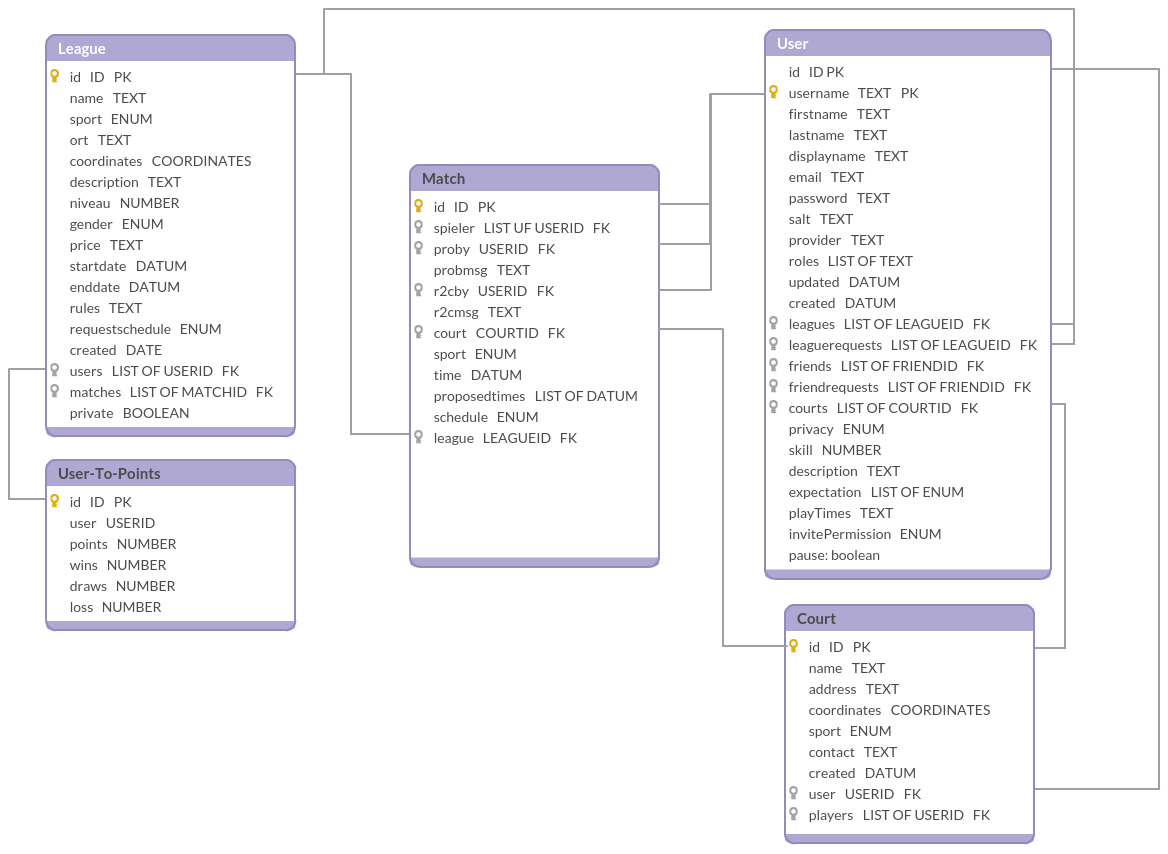
\includegraphics[width=0.9\textwidth]{Graphics/DBModel.png}
	\caption{Datenbank Modell}
	\label{DBMOdel}
\end{figure}

\newpage
\section{GUI}
Als GUI wird ein standard Bootstrap Design verwendet. Ohne Authentisierung kann nur die Home-Page gesehen werden sowie die Login und Signup Page. F�r alle anderen Seiten muss der Benutzer authentisiert sein. Sobald die Authentisierung durchgef�hrt wurde, gibt es k�nnen die Elemente (Nach Datenbank) Benutzer, Liga, Racketsportzentrum sowie Spiele selektiert werden. Innerhalb der einzelnen Menu kann man verschiedene Operationen direkt ansteuern, einige nur �ber andere Operationen. Folgendes Diagram zeigt die Interaktion durch die verschiedenen Views.
\begin{figure}[ht]
	\centering
	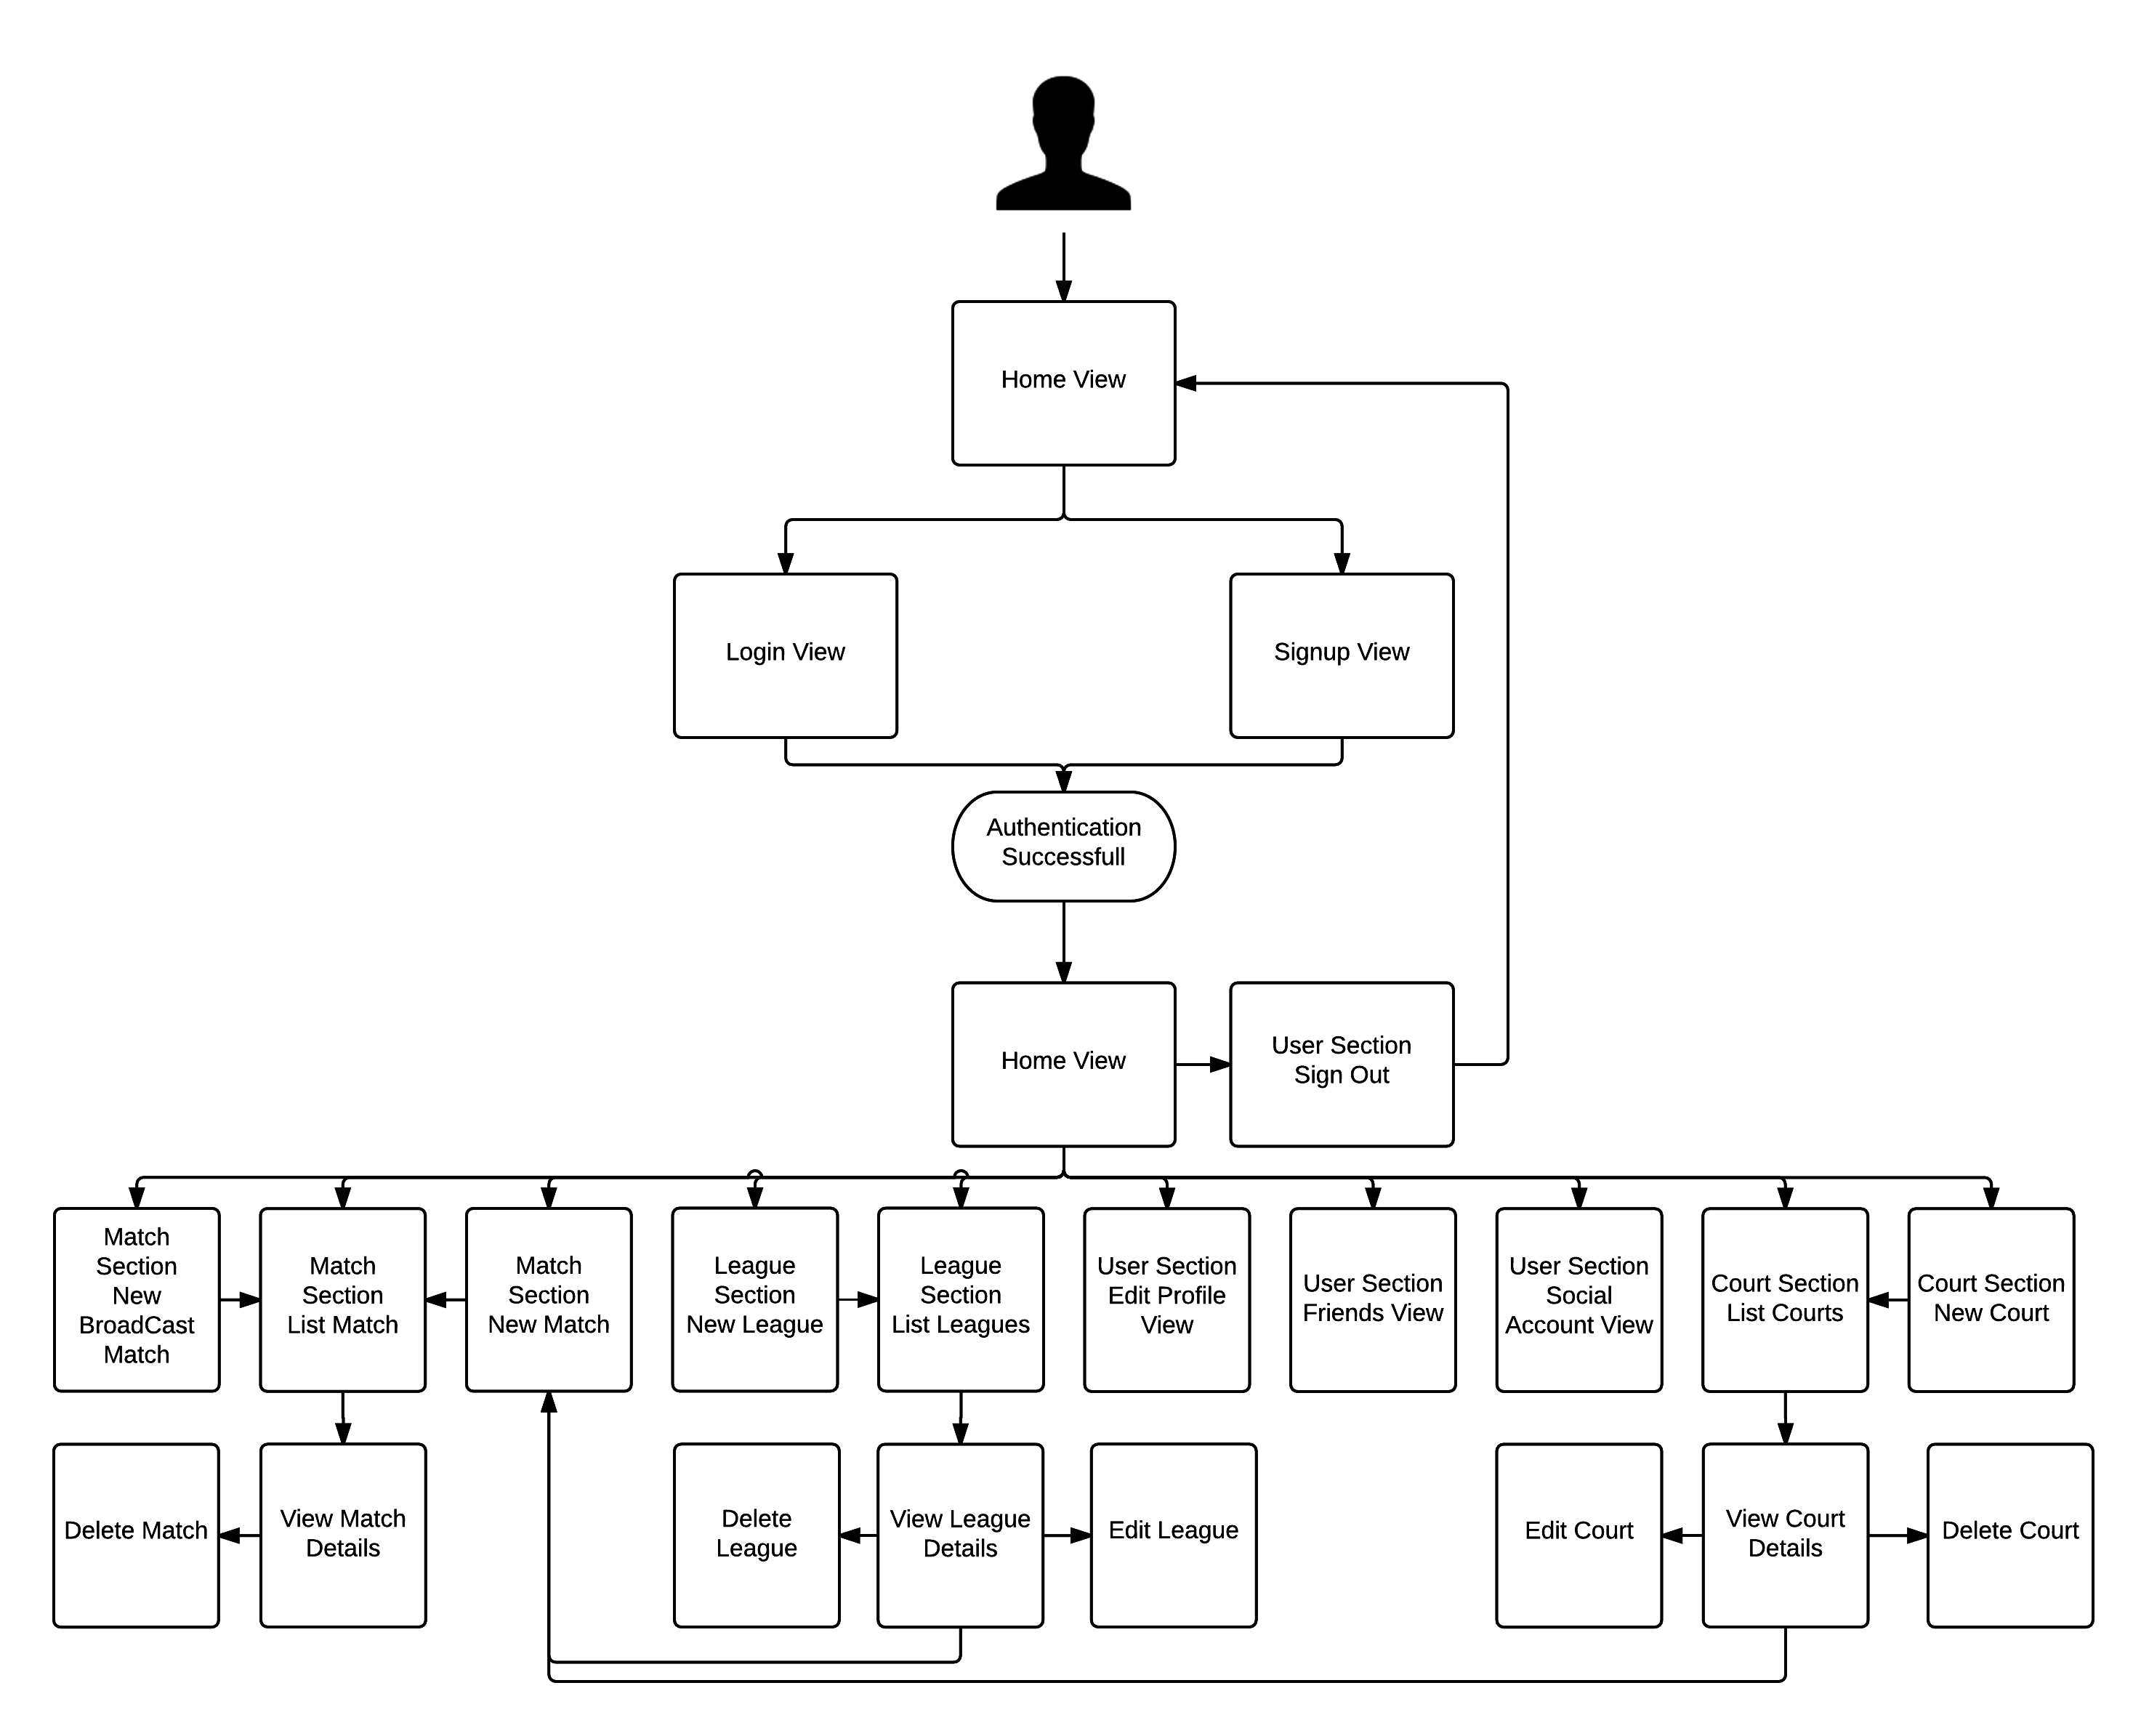
\includegraphics[width=0.9\textwidth]{Graphics/GUIInteraction.png}
	\caption{GUI Interaktions Modell}
	\label{GUIInteraction}
\end{figure}

\subsection{User Section}
Die User Section einhaltet drei Views die direkt aus dem Menu erreichbar sind. Die erste View User Profile erm�glicht dem User, Details �ber sich preiszugeben. Er kann zus�tzlich das Passwort �ndern. Inder Friends view kann er neue Friendrequests erstellen, und pendente Friendrequests annehmen oder ablehnen. Die Social Account View bietet eine Verkn�pfung von Social Accounts mit der Applikation an.

\subsection{Court Section}
Die Court Section beinhaltet vier Views sowie eine Aktion. In der new Court View kann ein neues Racketsportzentrum registriert werden. In der List Courts view findet man alle  Racketsportzentren und erreicht bei klick auf ein Zentrum die View Court Details View. In dieser View kann man alle Details des Racketsportzentrum anschauen, sowie alle Spieler, welche in diesem Racketsportzentrum spielen. Durch klick auf den Spieler kann in die New Match View gewechselt werden, um einen Spieler herauszufordern. Von der Detail View kann man zus�tzlich das Court l�schen, sofern man das Court erstellt hat oder ein Admin ist.

\subsection{League Section}
Die League Section beinhaltet vier Views sowie eine Aktion. In der New League View kann ein neues Liga registriert werden. In der List League View findet man alle  Ligen und erreicht bei klick auf eine Liga die View League Details View. In dieser View kann man alle Details die Liga anschauen, sowie alle Spieler, welche in dieser Liga spielen. Durch klick auf den Spieler kann in die New Match View gewechselt werden, um einen Spieler herauszufordern. Von der Detail View kann man zus�tzlich die Liga l�schen, sofern man die Liga erstellt hat oder ein Admin ist.

\subsection{Match Section}
Die Match Section beinhaltet alle Interaktionen im Match. Drei Views sind direkt aus dem Menu erreichbar. Auf der New Match View kann man ein neues Spiel erstellen. Man kann Court, Spieler in einem Formular ausw�hlen. �ber den Menupunkt New Broadcast Match View, w�hlt man ein Court sowie eine Zeit und alle Spieler, welche in diesem Court spielen werden angefragt f�r eine spontanes Spiel. In der List Match View werden alle Spiele aufgelistet. Von da kommt man in die View Match Details View, welche den Matchworkflow abdeckt.


% !TeX spellcheck = de_CH
\chapter{Implementation}

\section{Projektaufbau}
Um den Projektaufbau zu erkl�ren wird zuerst die Ordnerstruktur angeschaut:
\begin{figure}[ht]
	\centering
	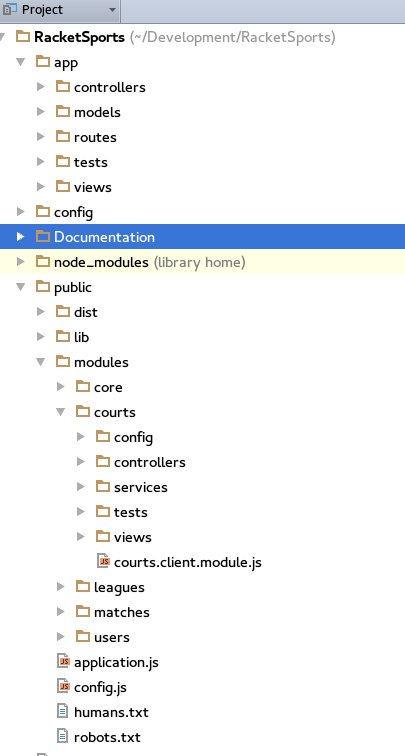
\includegraphics[width=0.3\textwidth]{Graphics/projectsetup.png}
	\caption{Projekt Ordner Struktur}
	\label{ProjectSetup}
	\end{figure}
Wie auf der Graphik ersichtlich besteht das Projekt aus den �berordnern App, Documentation und public. Node\textunderscore modules ist ein System-Ordner und muss hier nicht betrachtet werden.
\subsection{app}


\begin{itemize}
	\itemsep-0.4em
	\item Controller - Kontroller im MVC
	\item Models - Definition der Datenobjekte
	\item Routers - Routing definition durch das MVC
	\item Tests - Unittests f�r Controller und Models
	\item Views - Verschiedene Basisviews, welche noch nicht zum Client gesendet wurden
\end{itemize}

\subsection{Documentation}
Der Ordner Documentation beinhaltet diese Dokumentation sowie alle Pr�sentationen.

\subsection{public}
Public beinhaltet alle Files, welche an den Client gesendet werden.
\begin{itemize}
	\itemsep-0.4em
	\item dist - Beinhaltet definitionen, welche Ordner gesendet werden, was f�r Module wo registriert werden sollen
	\item lib - binhaltet statische Libraries, welche der Client braucht. Hier befinden sich nodeJS, AngularJS und Bootstrap als libraries.
	\item modules - Hier ist die Eigentliche Client Logik versteckt. F�r jedes Modul gibt es folgende Ordner:
	\begin{itemize}
	\itemsep -0.4 em
		\item config - Konfiguration von Modul und Client Routing. Definiert z.b. was f�r Items �ber den Header ansprechbar sind
		\item controller - AngularJS Controller
		\item services - Definiert den Link zur API
		\item tests - Unit Tests f�r die AngularJS Module
		\item views - Definiert views f�r die einzelnen Seiten der Applikation.
	\end{itemize}

\end{itemize}

\section{REST API}
Die REST API besteht aus f�nf Endpunkten:
\begin{itemize}
	\itemsep-0.8em
	\item /matches - Stellt alle Operationen f�r Matches zur Verf�gung
	\item /leagues - Stellt alle Operationen f�r Liga Management zur Verf�gung
	\item /courts - Stellt alle Operationen f�r die Verwaltung von Racketsportzentren zur Verf�gung
	\item /users - Stellt alle Operationen f�r das Usermanagemnt zur Verf�gung
	\item /core - Stellt Core-Funktionalit�ten (Home Seite) zur Verf�gung
\end{itemize}
Die Endpunkte /users und /core waren im MEANJS Stack schon vorhanden. Der User Endpunkt wurde jedoch modifiziert. Die Modifizierungen sind in dem Kapitel dokumentiert, die schon vorhandenen Endpunkte nicht. 

\subsection{Routing}
Um die REST API anzusteuern gibt es ein zentrales Routing in der Applikation. Dieses Routing definiert, welche URL welche Funktion aufruft. Jedes Modul hat eine eigene Routing Definition um das die einzelnen Files �bersichtlich zu halten. 

Folgendes Codebeispiel zeigt das Routing des Courts Moduls. Es definiert URLs und HTTP Methoden wie die URL aufgerufen wird. Je nach Methode werden anschliessend verschiedene Parameter definiert, zum Beispiel wie der Endpunkt gesch�tzt ist (requires Login, hat Autorisierung) und anschliessend welche Funktion aufgerufen wird (courts.update)

\begin{lstlisting}
module.exports = function(app) {
var users = require('../../app/controllers/
		users.server.controller');
var courts = require('../../app/controllers/
		courts.server.controller');

// Courts Routes
app.route('/courts')
.get(courts.list)
.post(users.requiresLogin, courts.create);

app.route('/courts/:courtId')
.get(courts.read)
.put(users.requiresLogin, courts.hasAuthorization, courts.update)
.delete(users.requiresLogin, courts.hasAuthorization,
 courts.delete);
app.route('/courts/:courtId/join')
.get(users.requiresLogin, courts.join);
app.route('/courts/:courtId/leave')
.get(users.requiresLogin, courts.leave);
// Finish by binding the Court middleware
app.param('courtId', courts.courtByID);
};

\end{lstlisting}

Am Anfang (Linie 2 und 4) der Routen werden die Controller inkludiert, damit die Funktionen auch gefunden werden.


\subsection{Spiel Endpunkt /matches}
\begin{figure}[ht]
	\centering
	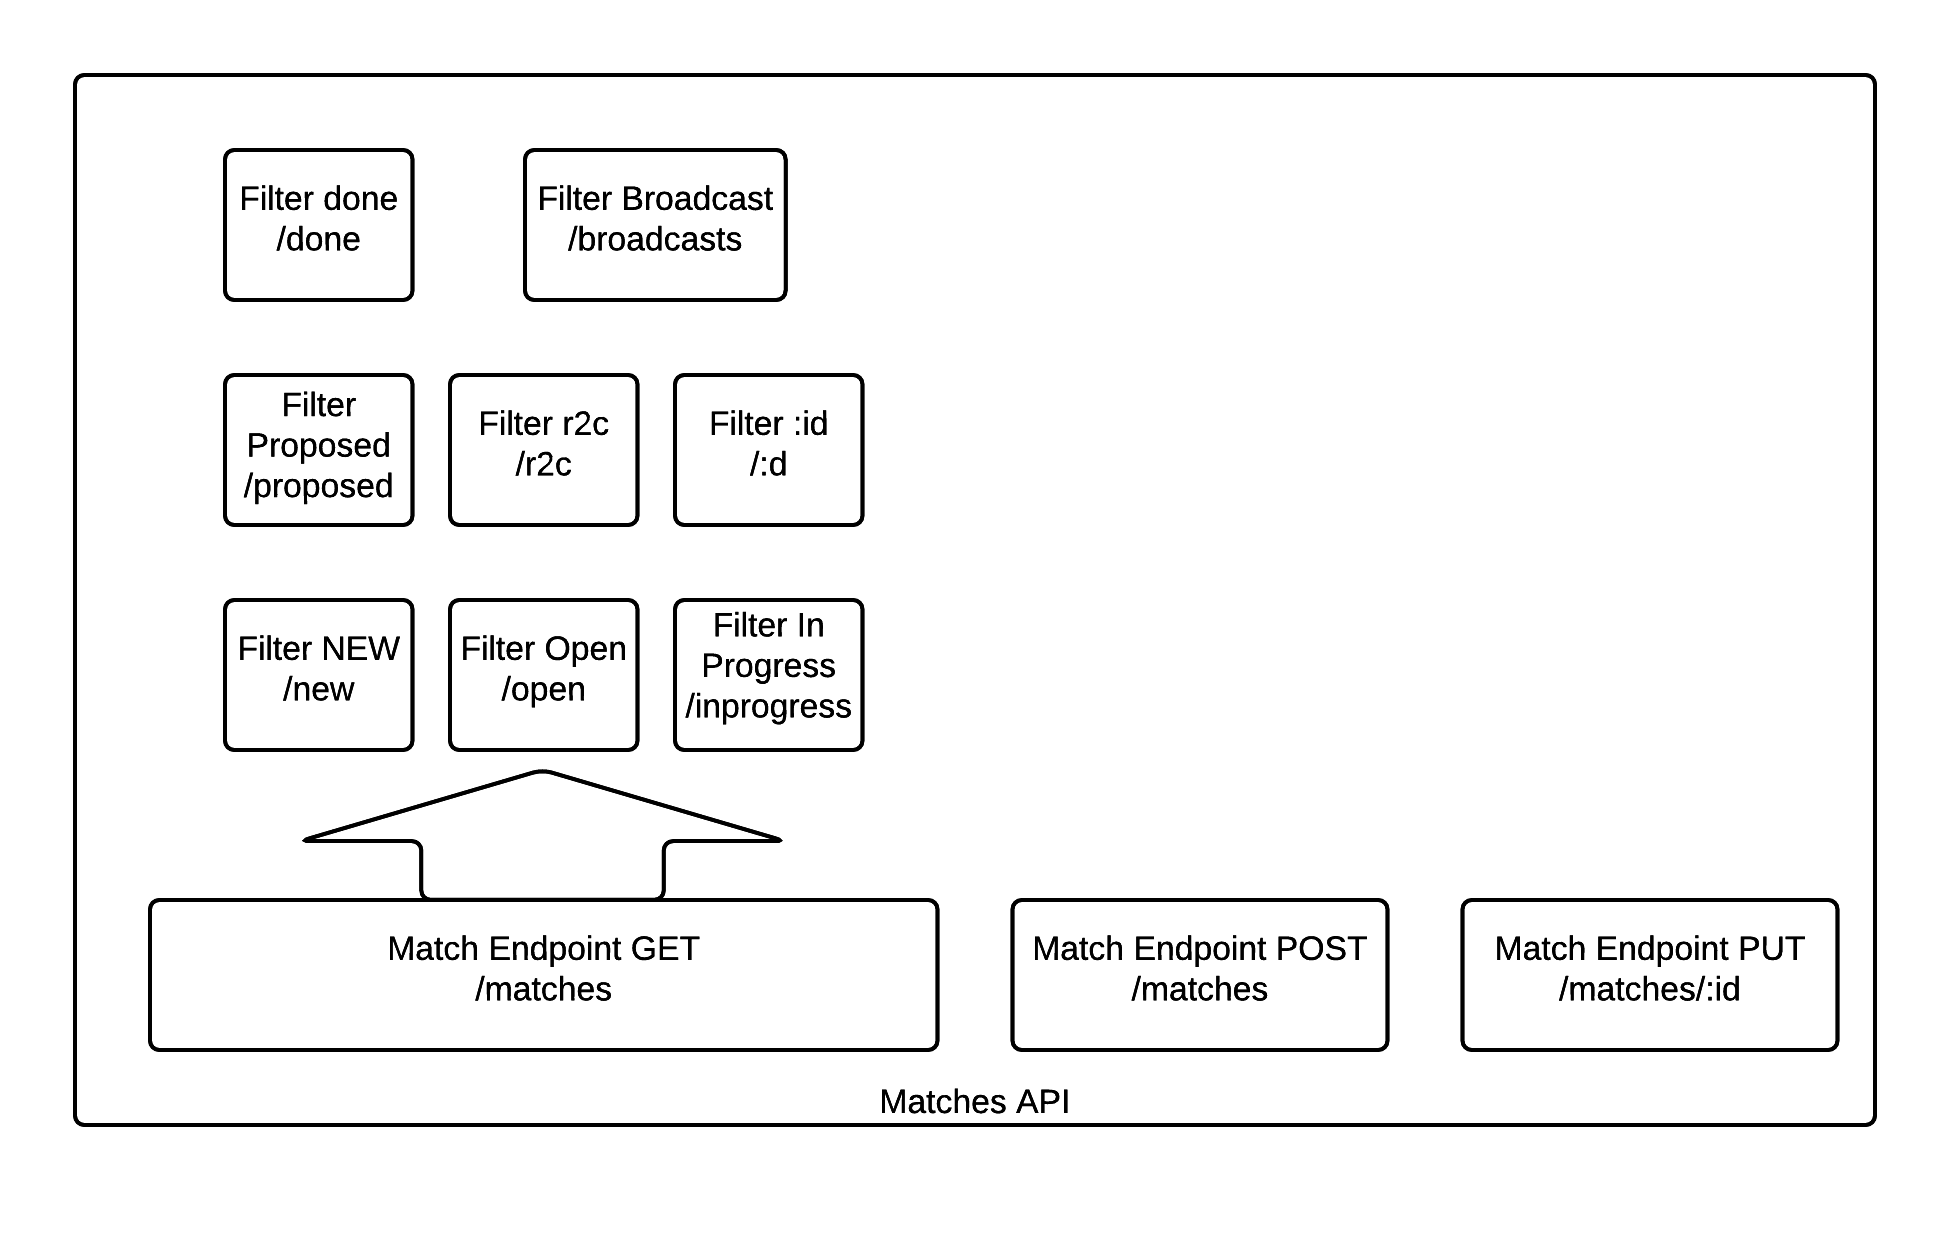
\includegraphics[width=0.8\textwidth]{Graphics/api_match.png}
	\caption{API f�r Spiele}
	\label{MatchAPI}
\end{figure}

Bei allen Match Endpunkten muss der User als Spieler registriert sein, um Informationen �ber das Spiel zu erhalten. Ausnahme ist, wenn er direkt die ID eingibt und direkt auf Spiel Detauls zugreift. 

Mit einem Post f�gt man der Datenbank ein Spiel hinzu, mit PUT aktualisiert man das Spiel mit neuen oder ge�nderten Daten. Hinter dem PUT interface gibt es gewisse Input Validations um Missbrauch zu verhindern. In dieser ersten Version sin ddie Validations jedoch relativ einfach gehalten. 

Um eine gute �bersicht aller Spiele auf der List Matches View zu erstelllen, gibt es f�r jeden Status eines Spieles einen eigenen API Call (/matches/new, /matches/open, /matches/inprogress, /matches/proposed, /matches/r2c, /matches/done). 

Der API Endpunkt /matches/broadcast listet zus�tzlich alle broadcasting Anfragen auf. Der Conntroller des Enpunkt Korreliert, in welchen Racketsportzentren der User registriert ist und die Matches ohne zweiten Spieler und gibt das Resultat dem Client.

\subsubsection{Codebeispiel - Filtering und Population von Unterobjekten}
Um bei den Spielen nur die offene Spiele zu finden, wird in der Datenbank auf den Status des Spiels gefiltert. Dies wird �ber einen Select auf die JSON Eigenschaft gemacht:
\begin{lstlisting}
exports.listOpen = function(req, res) {
	var user = req.user;
Match.find({'spieler.user': req.user, state: 'open'})
	.sort('-created').populate('spieler court')
	.exec(function(err, matches) {
		User.populate(matches, {path: 'spieler.user'},
		function (err, user) {
		if (err) {
			return res.status(400).send({
			message: errorHandler.getErrorMessage(err)
		});
		} else {
			res.jsonp(matches);
		}
		});
	});
};
\end{lstlisting}
Auf der Zeile 3 ist der Select f�r die Datenbank zu finden. Ein Teil des zu suchenden Objektes wird definiert als erster Parameter der Match.find() Methode.

Das Match Objekt beinhaltet Spieler sowie Courts. Diese Felder sind jedoch nur IDs auf andere Objekte (Als Beispiel: ObjectID(AA4335GE0DE9EV88A) ). Um auf Datenfehler der Unterobjekte zugreifen zu k�nnen, m�ssen die Objekte popularisiert werden. Auf der Zeile 4 erkennt man, dass f�r das Objekt Match die Unterobjekte Spieler sowie Courts popularisiert werden. Nun hat das Objekt Spieler zus�tzlich Unterobjekte. Hier muss man eine neue Population des Objektes User ausf�hren (siehe Zeile 6).



\subsection{Liga Endpunkt}

\begin{figure}[ht]
	\centering
	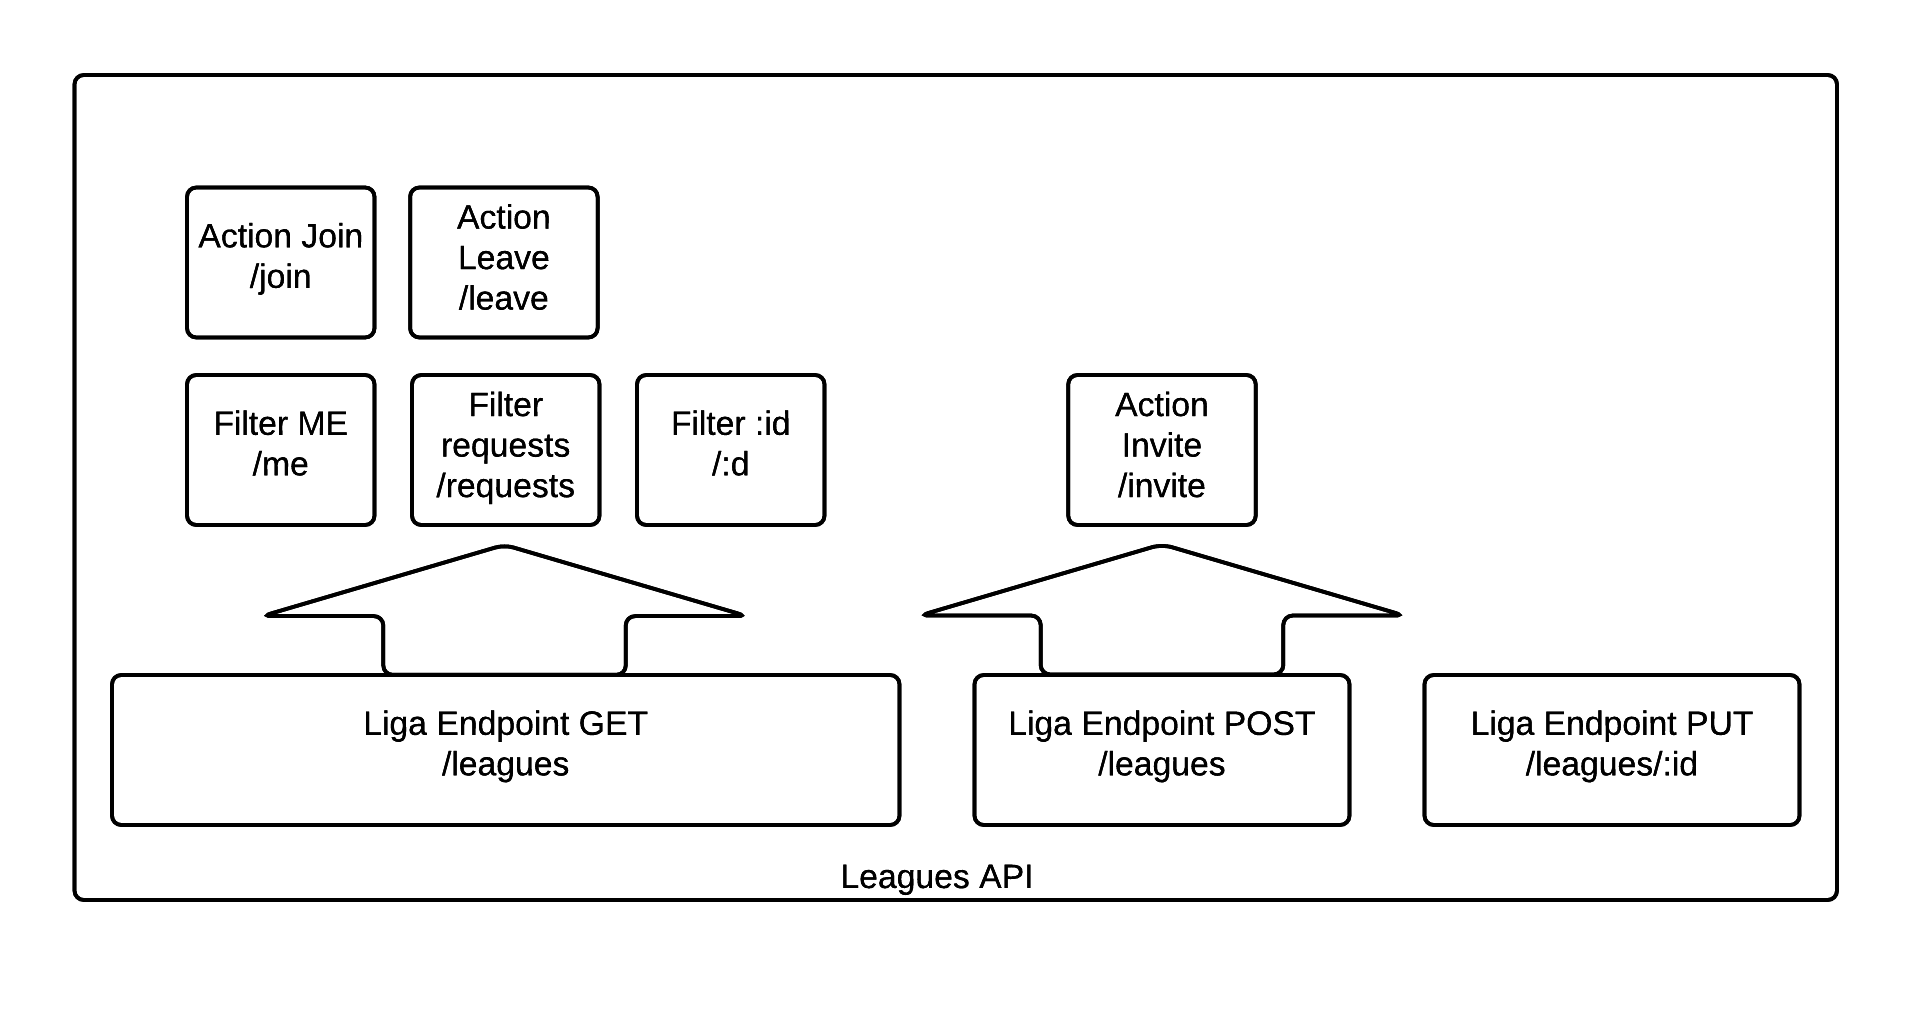
\includegraphics[width=0.8\textwidth]{Graphics/api_league.png}
	\caption{API f�r Ligen}
	\label{LeagueAPI}
	\end{figure}

Bei der Liga gibt es - wie bei allen Endpunkten - CRUD Endpunkte (/leagues f�r list all, /leagues/:id f�r Show Element, POST /leagues f�r Create League, PUT /leagues/:id f�r Update League). Zus�tzlich gbit es eine Join Action, welche den authentisierten User einer Liga hinzuf�gt sowie ein Leave Endpunkt um die Registriertung zu l�schen.

Ein zus�tzlicher Endpunkt ist /leagues/invite, welcher erm�glicht einen User zu einer Liga einzuladen.

\subsubsection{Codebeispiel - Join/Leave Funktionen}

Die Join/Leave Funktionalit�t besteht aus zwei API Endpunkten. Wenn man nun die URL /leagues/join aufruft, wird folgender Code ausgef�hrt:

\begin{lstlisting}
exports.join = function (req, res) {

    var league = req.league;
    var user = req.user;
    var userToPoints = new UserToPoints();
    userToPoints.user = req.user;
    userToPoints.save();

    league.users.push(userToPoints);
    user.leagues.push(league)

    console.log(league);
    league.save(function (err) {
        ....
\end{lstlisting}

Auf der Zeile 3 und 4 werden User und Liga aus dem Request gelesen. Diese Daten werden implizit von AngularJS mitgeliefert. 

Nun wird ein neues Liga-Spieler Objekt, ein Objekt welches den Spieler und seine Ranglistenpunkte beinhaltet erstellt und gespeichert (Zeile 5-7). Dieses Objekt wird nun in die Liste aller Liga-Spieler Objekte hinzugef�gt und die Liga wird abgespeichert (Zeile 13).

\begin{lstlisting}
exports.leave = function (req, res) {
    var league = req.league;
    var user = req.user;
    var i = league.users.indexOf(req.user);
    league.users.splice(i, 1);
    var j = user.leagues.indexOf(req.league);
    user.leagues.splice(j, 1);
    league.save(function (err) {
    ....
\end{lstlisting}
Will ein User die Liga verlassen, wird sein Objekt aus der Liste von Spielern gel�scht.

	\newpage
\subsection{Racketsportzentrum Endpunkt /courts}
\begin{figure}[ht]
	\centering
	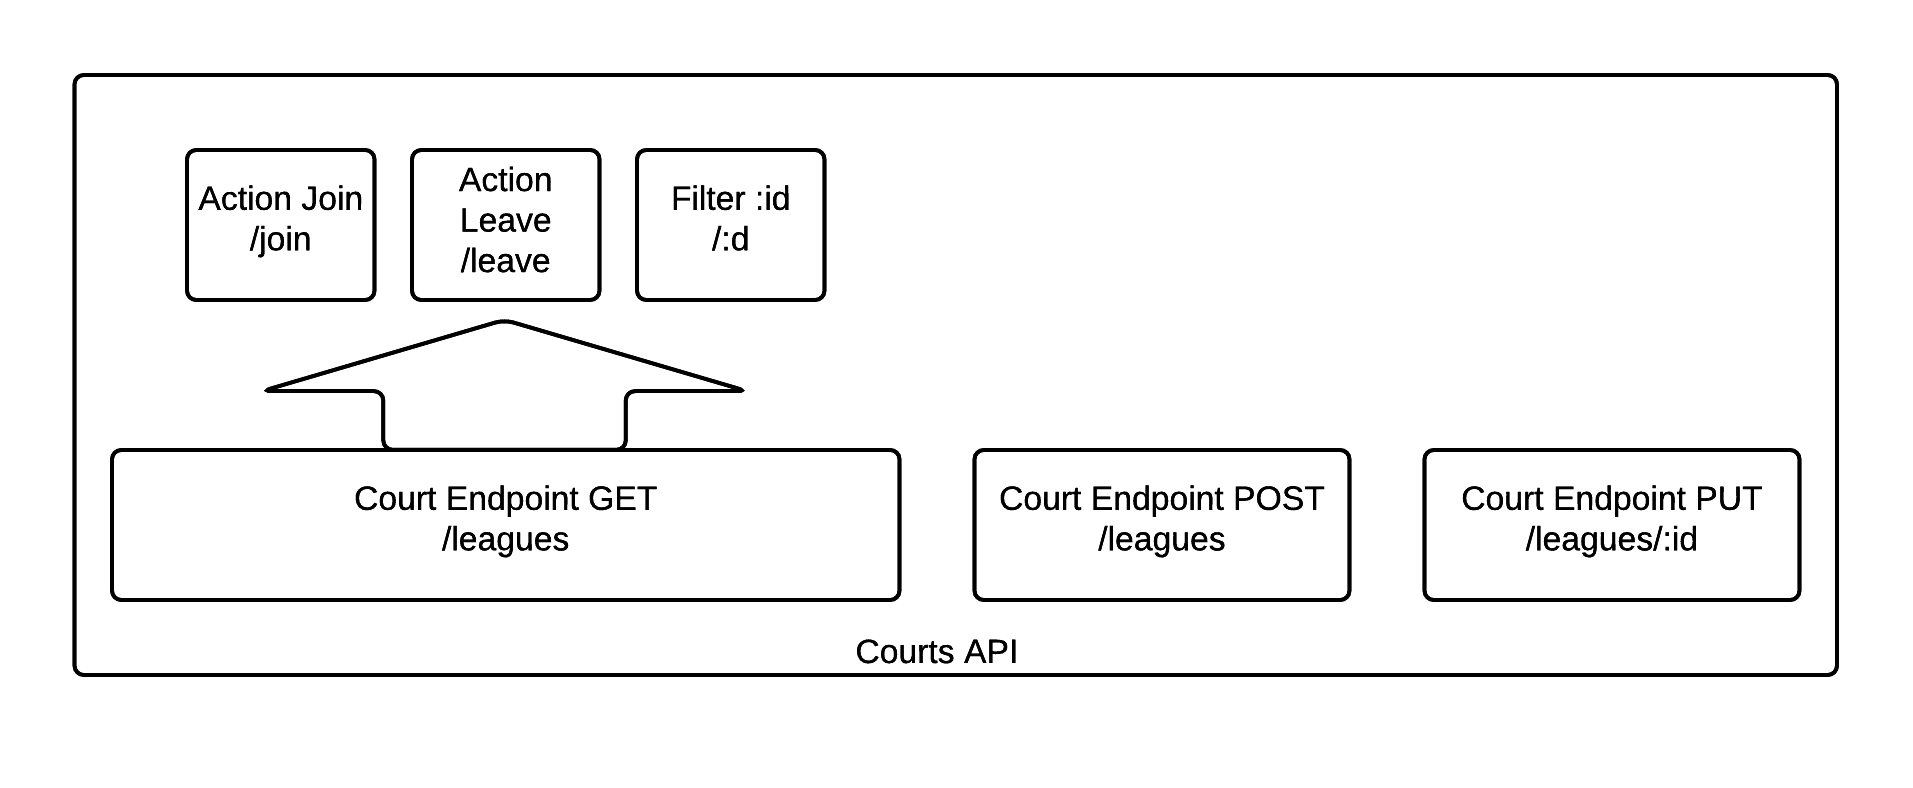
\includegraphics[width=0.8\textwidth]{Graphics/api_court.png}
	\caption{API f�r Racketsportzentren}
	\label{CourtAPI}
\end{figure}
Gleich wie beim Liga Endpunkt gibt es die CRUD Endpunkte sowie ein Join/Leave Endpunkt

\subsection{Benutzer Endpunkt /users}
Neben den �blichen Benutzerverwaltungs Endpunkten (/user/signin, /user/signout, /user signup, /auth/forgot), welche hier nicht Dokumentiert werden, gibt es Endpunkte f�r das Freunde-System:
\begin{itemize}
	\itemsep-0.5em
	\item GET /users/friend - Auflistung aller Freunde
	\item DELETE /users/friend - L�schen eines Freundes
	\item GET /users/request -  Senden eines Freund Requests
	\item DELETE /users/request - L�schen eines Freund Requests
\end{itemize}

\subsubsection{Codebeispiel - OAuth Integration}
Der MEAN Stack bietet ein OAuth Integrations Plugin an. Man muss nur noch das Plugin konfigurieren. Daf�r wird f�r jeden Authentication Provider eine Strategie definiert:
\begin{lstlisting}
....
	GoogleStrategy = require('passport-google-oauth').OAuth2Strategy,
....
module.exports = function() {
	// Use google strategy
	passport.use(new GoogleStrategy({
			clientID: config.google.clientID,
			clientSecret: config.google.clientSecret,
			callbackURL: config.google.callbackURL,
			passReqToCallback: true
		},
		function(req, accessToken, refreshToken, profile, done) {
			// Set the provider data and include tokens
			var providerData = profile._json;
			providerData.accessToken = accessToken;
			providerData.refreshToken = refreshToken;

			// Create the user OAuth profile
			var providerUserProfile = {
				firstName: profile.name.givenName,
				lastName: profile.name.familyName,
				displayName: profile.displayName,
				email: profile.emails[0].value,
				username: profile.username,
				provider: 'google',
				providerIdentifierField: 'id',
				providerData: providerData
			};

			// Save the user OAuth profile
			users.saveOAuthUserProfile(req, providerUserProfile, done);
		}
	));
};
\end{lstlisting}

Die Daten werden bei Registrierung �ber OAuth in das Userprofil abgelegt. (Siehe Zeile 19-27 ). Zus�tzlich ist es n�tig bei jedem Provider ein Access Token anzufordern und in die Produktionsumgebung der Applikation einzupflegen.

\section{Web Applikation}

Die WebApplikation ist wie bereits erw�hnt mit Bootstrap und AngularJS programmiert. In AngularJS werden Direktiven erstellt, um einzelne API Endpunkte anzusprechen und diese Realtime in die View zu injecten. Hier ein Beispiel einer Direktive:
\begin{lstlisting}
$scope.find = function() {
			$scope.courts = Courts.query();
		};

\end{lstlisting}

Wenn die Operation find() in der View aufgerufen wird, erstellt AngularJS eine Query zum Endpunkt /courts und bekommt alle Court Objekte zur�ck. Diese Courtobjekte werden nun in die globale Variable courts im \textdollar scope abgef�llt. AngularJS updatet nun die View, welche die Variable courts anzeigt:
\begin{lstlisting}
<section data-ng-controller="CourtsController" data-ng-init="find()">
    ....
        <table id="courtslist" class="table">
            <tr>
                <th>Name</th><th>Adresse</th><th>Verf�gbare Sportarten</th>
            </tr>

            <tr data-ng-repeat="court in courts" id="{{court._id}}" ng-click="go(court)"  onMouseover="this.bgColor='#DDDDDD'" onMouseout="this.bgColor='#FFFFFF'">
                <td data-ng-bind="court.name"></td>
                <td data-ng-bind="court.address"></td>
                <td data-ng-bind="court.sports"></td>
            </tr>
        </table>
....
\end{lstlisting}

Das ganze Webinterface ist auf solchen Direktiven aufgebaut.

\subsection{Google Maps Integration}
 Eine Adresse wie z.B. \lq Vitis \rq hat das Problem, dass man geographische N�he suchen kann. Darum ist es wichtig, das die Racketsport zentren ein Geographisch Valides Objekt haben. Um dies zu erreichen wurde die API von Google Maps integriert. Der Benutzer muss nun noch einem Objekt in Google Maps suchen, und dieses Selektieren um eine Valide Addresse zu bekommen. Folgendes Formularelement existiert in der View:
 \begin{lstlisting}
 <div class="form-group">
   <label for="address">Adresse</label>
   <input type="text" onFocus="geolocate()" id="address" name="address" class="form-control" data-ng-model="address" required>
 </div>
 \end{lstlisting}
 
 Wie auf Zeile 3 ersichtlich wird die direktive geolocate() aufgerufen. Diese Funktion ist Bestandteil der Google API, welche im Header von \url{https://maps.googleapis.com/maps/api/js?v=3.exp&signed_in=true&libraries=places} gedownloadet wird. Die ID address wird von dem Court Controller aufgerufen und folgender Listener wird hinzugef�gt:
 \begin{lstlisting}
 var placeSearch, autocomplete;
 		if(document.getElementById('address')) {
 			autocomplete = new google.maps.places.Autocomplete(
 				/** @type {HTMLInputElement} */(document.getElementById('address')));
 			// When the user selects an address from the dropdown,
 			// populate the address fields in the form.
 
 			google.maps.event.addListener(autocomplete, 'place_changed', function () {
 				$scope.updateAddress();
 			});
 		}
 \end{lstlisting}
Der autocomplete Listener ruft nun die AngularJS direktive updateAddress() auf:

\begin{lstlisting}
$scope.updateAddress =function() {
			var place = autocomplete.getPlace();
			document.getElementById('address').value = place.formatted_address;
			document.getElementById('lat').value = place.geometry.location.A;
			document.getElementById('lng').value = place.geometry.location.F;
			if ($scope.court) {
				$scope.court.address = place.formatted_address;
				$scope.court.lat = place.geometry.location.A;
				$scope.court.lng = place.geometry.location.F;
			}else{
				this.address = place.formatted_address;
				this.lat = place.geometry.location.A;
				this.lng = place.geometry.location.F;
			}
		};
\end{lstlisting}

UpdateAddress sucht das Google Maps Objekt und speichert die Values - Addresse sowie Koordinaten - in die View. Bei dem Abschicken des Formulares wird nun gepr�ft ob die Koordinaten existieren, falls nicht, ist es keine valide Adresse, wie man im Court-Model sieht (Zeile 3 und 7):
\begin{lstlisting}
lat: {
		type: String,
		required: "Please fill in a correct address (select it from the dropdown)"
	},
lng: {
		type: String,
		required: "Please fill in a correct address (select it from the dropdown)"
	}
\end{lstlisting}


\section{Android Applikation}
Als Grundlage f�r die Android Applikation wurde eine Applikation von gonative.io generiert. Im Laufe des Projektes - nach erheblicher �berschreitung des vorgeschriebenen Aufwandes - wurde entschieden keine vollst�ndig Native Webapplikation zu erstellen. Stattdessen wird eine WebView erstellt, welche die Mobile Webseite darstellt. Um alle Funktionalit�t zu behalten, wird �ber die WebView und Interception Algorithmen Push-Nachriten erm�glicht. Der einzige Setback ist, das die Website offline nicht verf�gbar ist.

\subsubsection{Codebeispiel - Push Interception}
TBD!!!!


\section{Workflows}
\section{Allgemeine Workflows}
\subsection{CRUD f�r Datenobjekte}
Alle Datenobjekte haben einen Endpunkt. Jeder Endpunkt stellt CRUD Operationen zur Verf�gung:
\begin{itemize}
	\itemsep -0.5em
	\item C - Neues Objekt erstellen
	\item R - Ein Objekt anzeigen
	\item U - Ein Objekt aktualisieren
	\item D - Ein Objekt l�schen
	\end{itemize}
	
	Zus�tzlich wird noch einen Endpunkt zur Auflistung aller Objekte angeboten. 

\newpage
\section{Court}
\subsection{Court Registrierung}
Wenn der User den Knopf im User Interface zur Registrierung das Racketsportzentrums dr�ckt, wird im Hintergrund der /courts/join API Call ausgef�hrt. Dieser Call f�gt der User der Anfrage in ein Array - bestehend aus allen registrierten Usern - ein. 
\begin{figure}[ht]
	\centering
	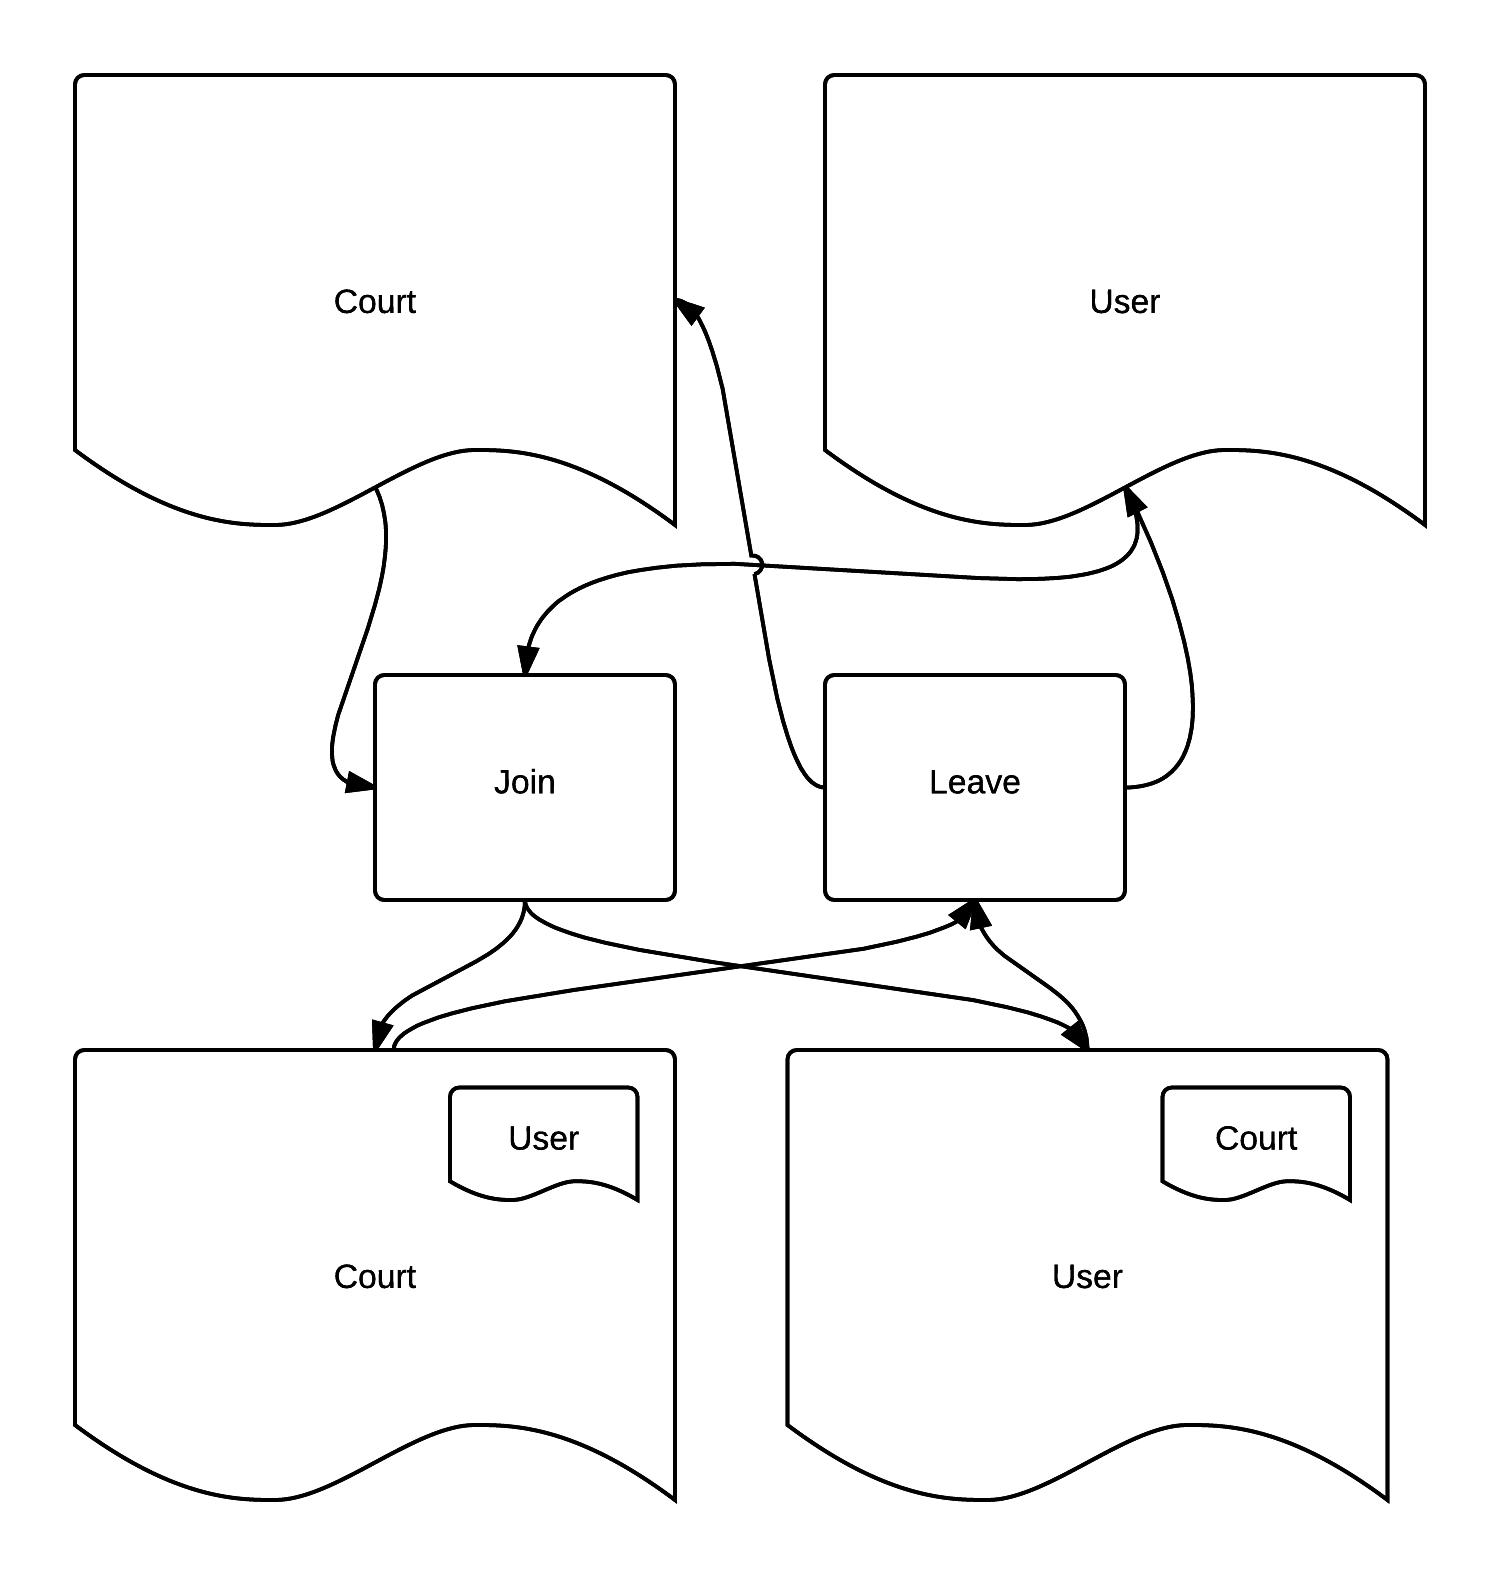
\includegraphics[width=0.7\textwidth]{Graphics/workflow_court.png}
	\caption{Racketsportzentrum Workflow}
	\label{CourtWorkflow}
\end{figure}
\newpage

\section{Liga}
\subsection{Liga Registrierung}
Identisch zu der Court Registrierung funktioniert die Liga Registrierung
\begin{figure}[ht]
	\centering
	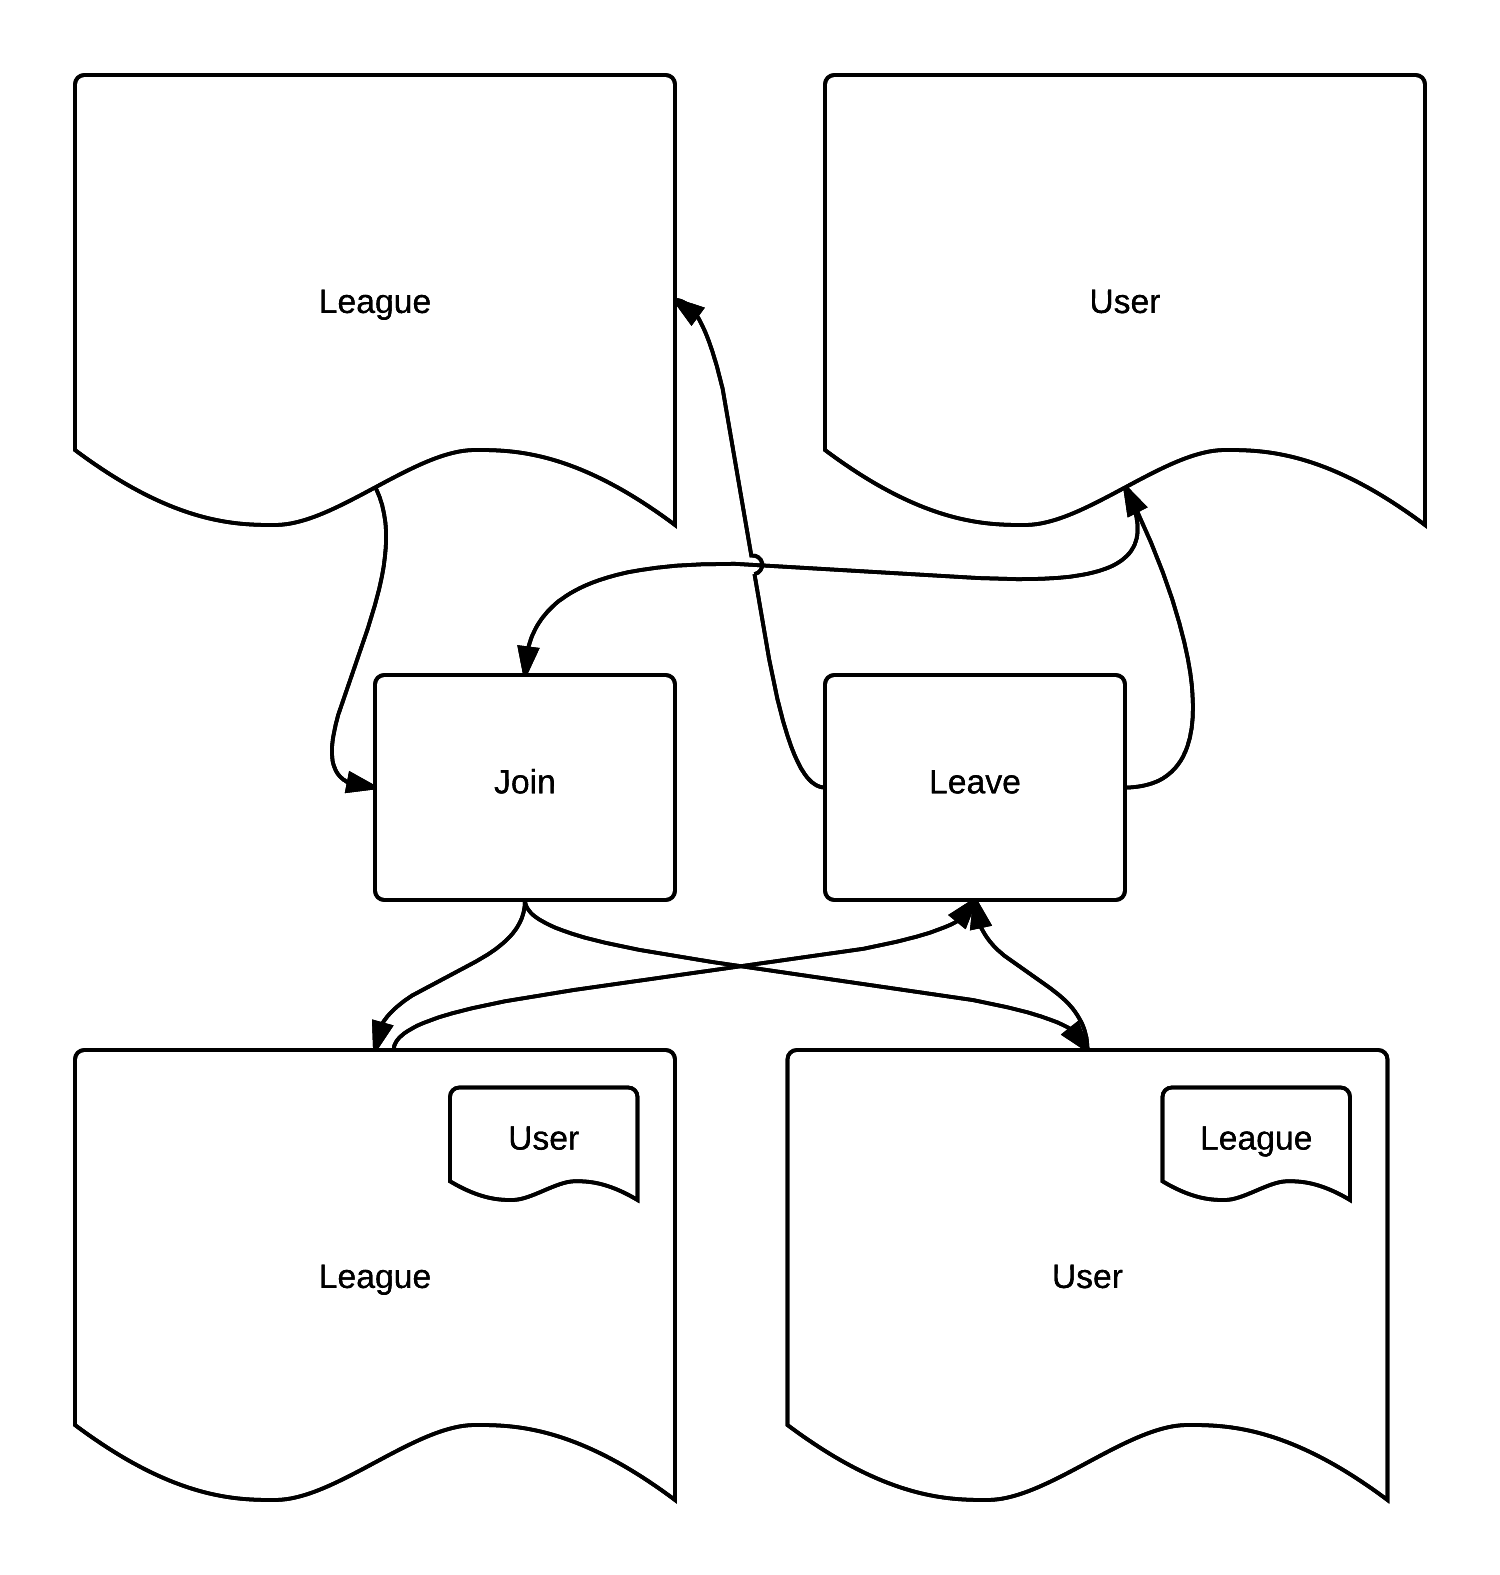
\includegraphics[width=0.7\textwidth]{Graphics/workflow_league.png}
	\caption{Liga Workflow}
	\label{LegueWorkflow}
\end{figure}

	\newpage
	\subsection{Automatische Herausforderung Liga}
	
	Bei der erstellung einer Liga kann ausgew�hlt werden ob automatische Herausforderungen aktiviert werden sollten. Aktuell gibt es vier verschiedene ausw�hlbare Modi:
	\begin{itemize}
		\item Weeklyall: W�chentliche Herausforderung, jeder gegen jeder, zuf�lliger Gegner
		\item Biweeklyall: Herausforderung alle zwei Wochen, jeder gegen  jeder, zuf�lliger Gegner
		\item WeeklyTopTwo: Herausforderung jede Woche, immer die zwei N�chsten in der Rangliste
		\item BiweeklTopTwo: Herausforderung alle zwei Wochen, immer die zwei N�chsten in der Rangliste
	\end{itemize}
	\begin{figure}[ht]
		\centering
		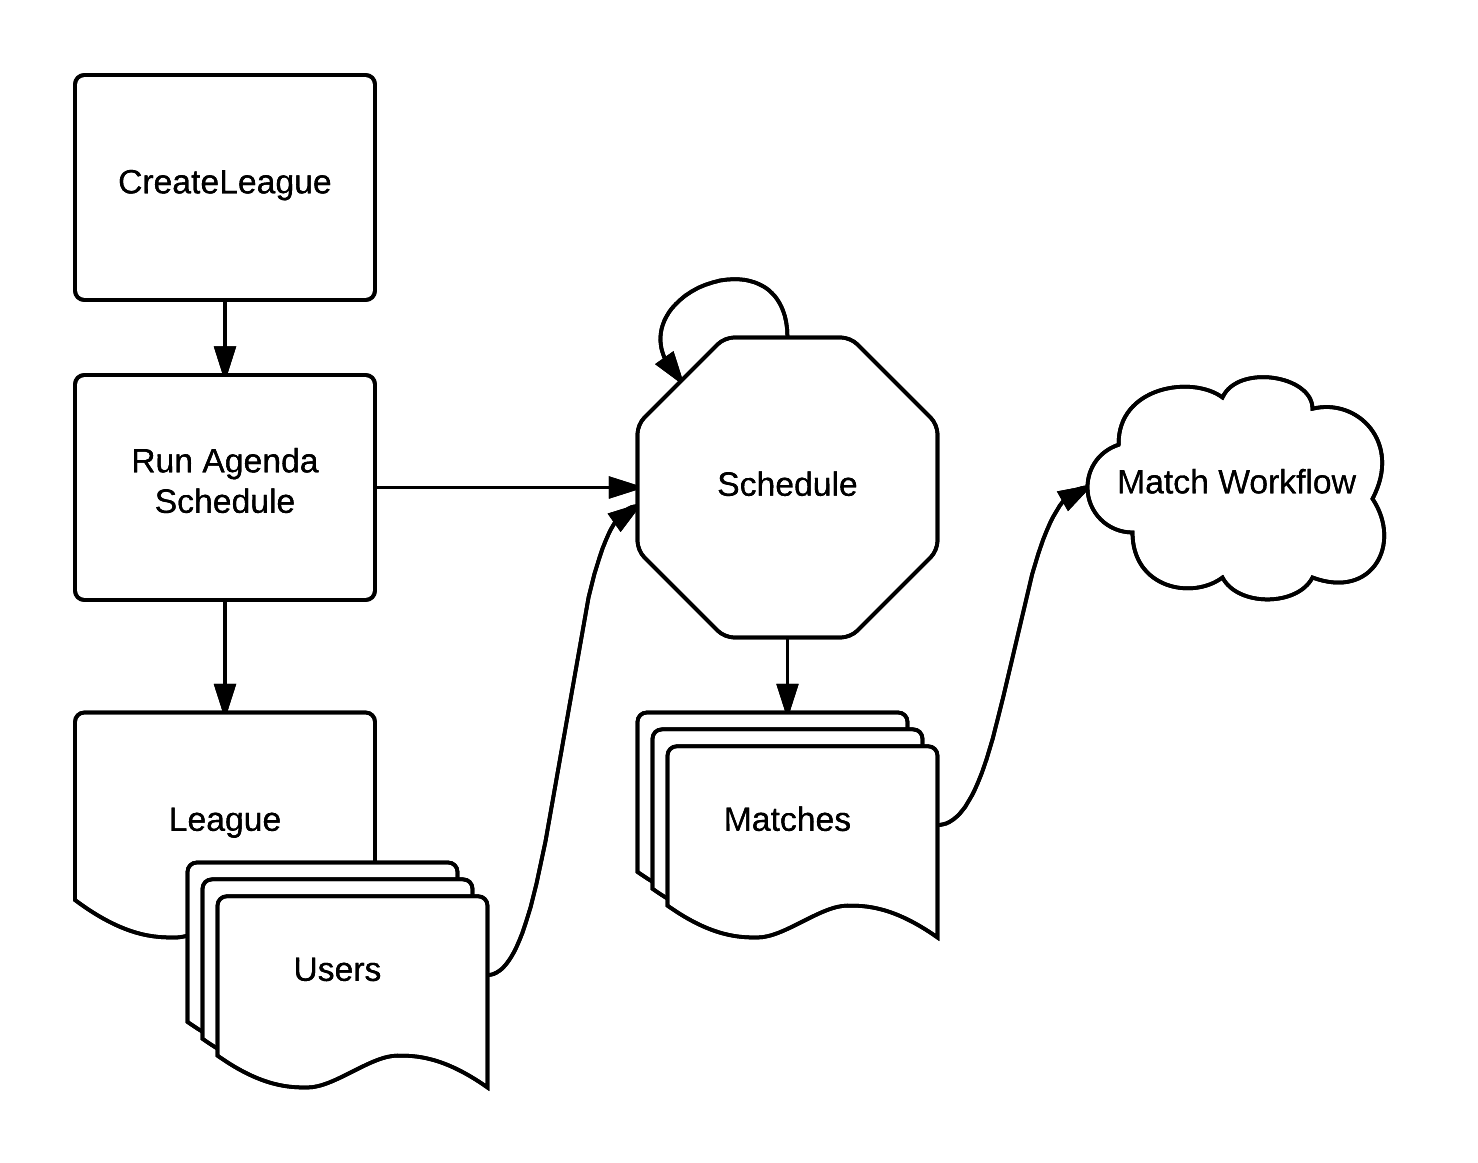
\includegraphics[width=0.7\textwidth]{Graphics/schedue_workflow.png}
		\caption{Schedule Workflow}
		\label{ScheduleWorkflow}
	\end{figure}
	\newpage
	\subsubsection{Codebeispiel - Scheduling}
	F�r das  Scheduling wird eine Externe Scheduling Libary f�r NodeJS gebraucht. Diese Library wird in den Startup der Applikation eingebunden:
\begin{lstlisting}
	var agenda = new Agenda({db: {address: config.dbagenda}});
	console.log("starting agenda");
	app.use('/agenda-ui', agendaUI(agenda, {poll: 1000}));
	agenda.start();
\end{lstlisting}
	Die Scheduling Libary - weiterf�hren Referenziert mit dem Namen Agenda - ben�tzt nun MongoDB um die Schedules zu persistieren. Wenn nun eine Liga erstellt wird, wird angegeben ob man Automatische Herausforderungen w�nscht. Falls dies gew�nscht ist, wird in der Funktion bei der Erstellung der Liga das Scheduling eingerichtet:
	\begin{lstlisting}
	if(league.requestShedule){
	    var agenda = new Agenda({db: {address: config.dbagenda}})
	    console.log("execute schedulematches sending ID: "+ league);
	    agenda.define(league._id+' schedule', League.scheduleMatches);
	    var job = agenda.create(league._id+' schedule',league.id);
	    if(league.requestShedule == 'weeklyAll'){
	        job.repeatAt('in 1 weeks');
	    }
	    if(league.requestShedule == 'biweeklyAll'){
	        job.repeatAt('in 2 weeks');
	    }
	    if(league.requestShedule == 'biweeklyTwoTop'){
	        job.repeatAt('in 2 weeks');
	    }
	    if(league.requestShedule == 'weeklyTwoTop'){
	        job.repeatAt('in 1 weeks');
	    }
	
	    //agenda.every('10 minutes', league._id+' schedule', league.id);
	
	    job.save()
	    agenda.start();
	}
	\end{lstlisting}
	
	\subsubsection{Random Herausforderungen / Rang Herausforderungen}
	Das Scheduling hat nun keinen Kontext der Applikation. Es beinhaltet nur das Model sowie alle Funktionen des Models. Aus diesem Grund wurde eine Funktion f�r das Starten der Herausforderungen innerhalb des Models erstellt:
	\begin{lstlisting}
	LeagueSchema.statics.scheduleMatches = function(job){
	    var League = mongoose.model('League'),
	        UserToPoints = mongoose.model('UserToPoints'),
	        Matches = mongoose.model('Match');
	    var leagueid = job.attrs.data;
	    League.findById(leagueid).populate("users").exec(function(err, league) {
	        UserToPoints.populate(league.users, {path: 'user', select: 'username'}, function (err, user) {
	
	            if (league) {
	                var l = league.users.length;
	                var player1, player2;
	                var k = league.users.length;
	                while (true){
	                if(league.requestShedule == 'biweeklyTwoTop' || league.requestShedule == 'weeklyTwoTop' ) {
	
	                        if (league.users.length > 1) {
	                             player1 = league.users[0].user;
	                            player2 = league.users[1].user;
	                            leage.users.splice(0,2);
	                        }
	                        else {
	                            break;
	                        }
	
	                }else {
	
	                        if (league.users.length > 1) {
	                            var p1 = Math.floor(Math.random() * l);
	                             player1 = league.users[p1].user;
	                            league.users.splice(p1, 1);
	                            l--;
	                            var p2 = Math.floor(Math.random() * l);
	                             player2 = league.users[p2].user;
	                            league.users.splice(p2, 1);
	                            l--;
	
	                        }
	                        else {
	                            break;
	                        }
	
	                    }
	                    var match = new Matches();
	                    match.spieler.push({user: player1});
	                    match.spieler.push({user: player2});
	                    match.sport = league.sport;
	                    match.league = league;
	                    match.state = 'new';
	                    match.save(function (err) {
	                        if (err) {
	                            console.log(err);
	                        }
	                    });
	                    if (l == 0) {
	                        break;
	                    }
	                }
	
	            } else {
	                console.log("no league with ID " + leagid + " found");
	            }
	        });
	    }
	    );
	
	}
	\end{lstlisting}
	Bis zur Zeile 9 sucht sich nun diese statische Funktion der Kontext aus der Datenbank zusammen. Es sucht sich selber, popularisiert die User und startet ab Zeile 14 das erstellen von Herausforderungen. 
	
	Je nach Modus (Random Herausforderungen, oder nach Rangliste) wird nun der Rangliste nach Spieler herausgefordert und diese aus der Rangliste gel�scht. Da das Liga Objekt nicht gespeichert wird, sind die �nderungen der Rangliste nur tempor�r. 
	
	Ist nun der Modus Random, wird das ganze etwas Komplexer. Zuerst wird aus der Rangliste ein Spieler zuf�llig ausgew�hlt (Zeile 28). Dieser Spieler wird nun von der Liste gel�scht und der Zeite Spieler wird ausgew�hlt (Zeile 32). Dieser wird nun auch gel�scht und der Match zwischen den zwei Spielern wird vereinbart. Das ganze wiederholt sich, bis keine Spieler mehr in der Rangliste sind. 
	
\begin{landscape}

\section{Match}
\subsection{Match Workflow}
Der Matchworkflow ist das Hauptelement der Applikation. Der Workflow regelt, wie der Match als Business Prozess durchgef�hrt wird. 
\begin{figure}[ht]
	\centering
	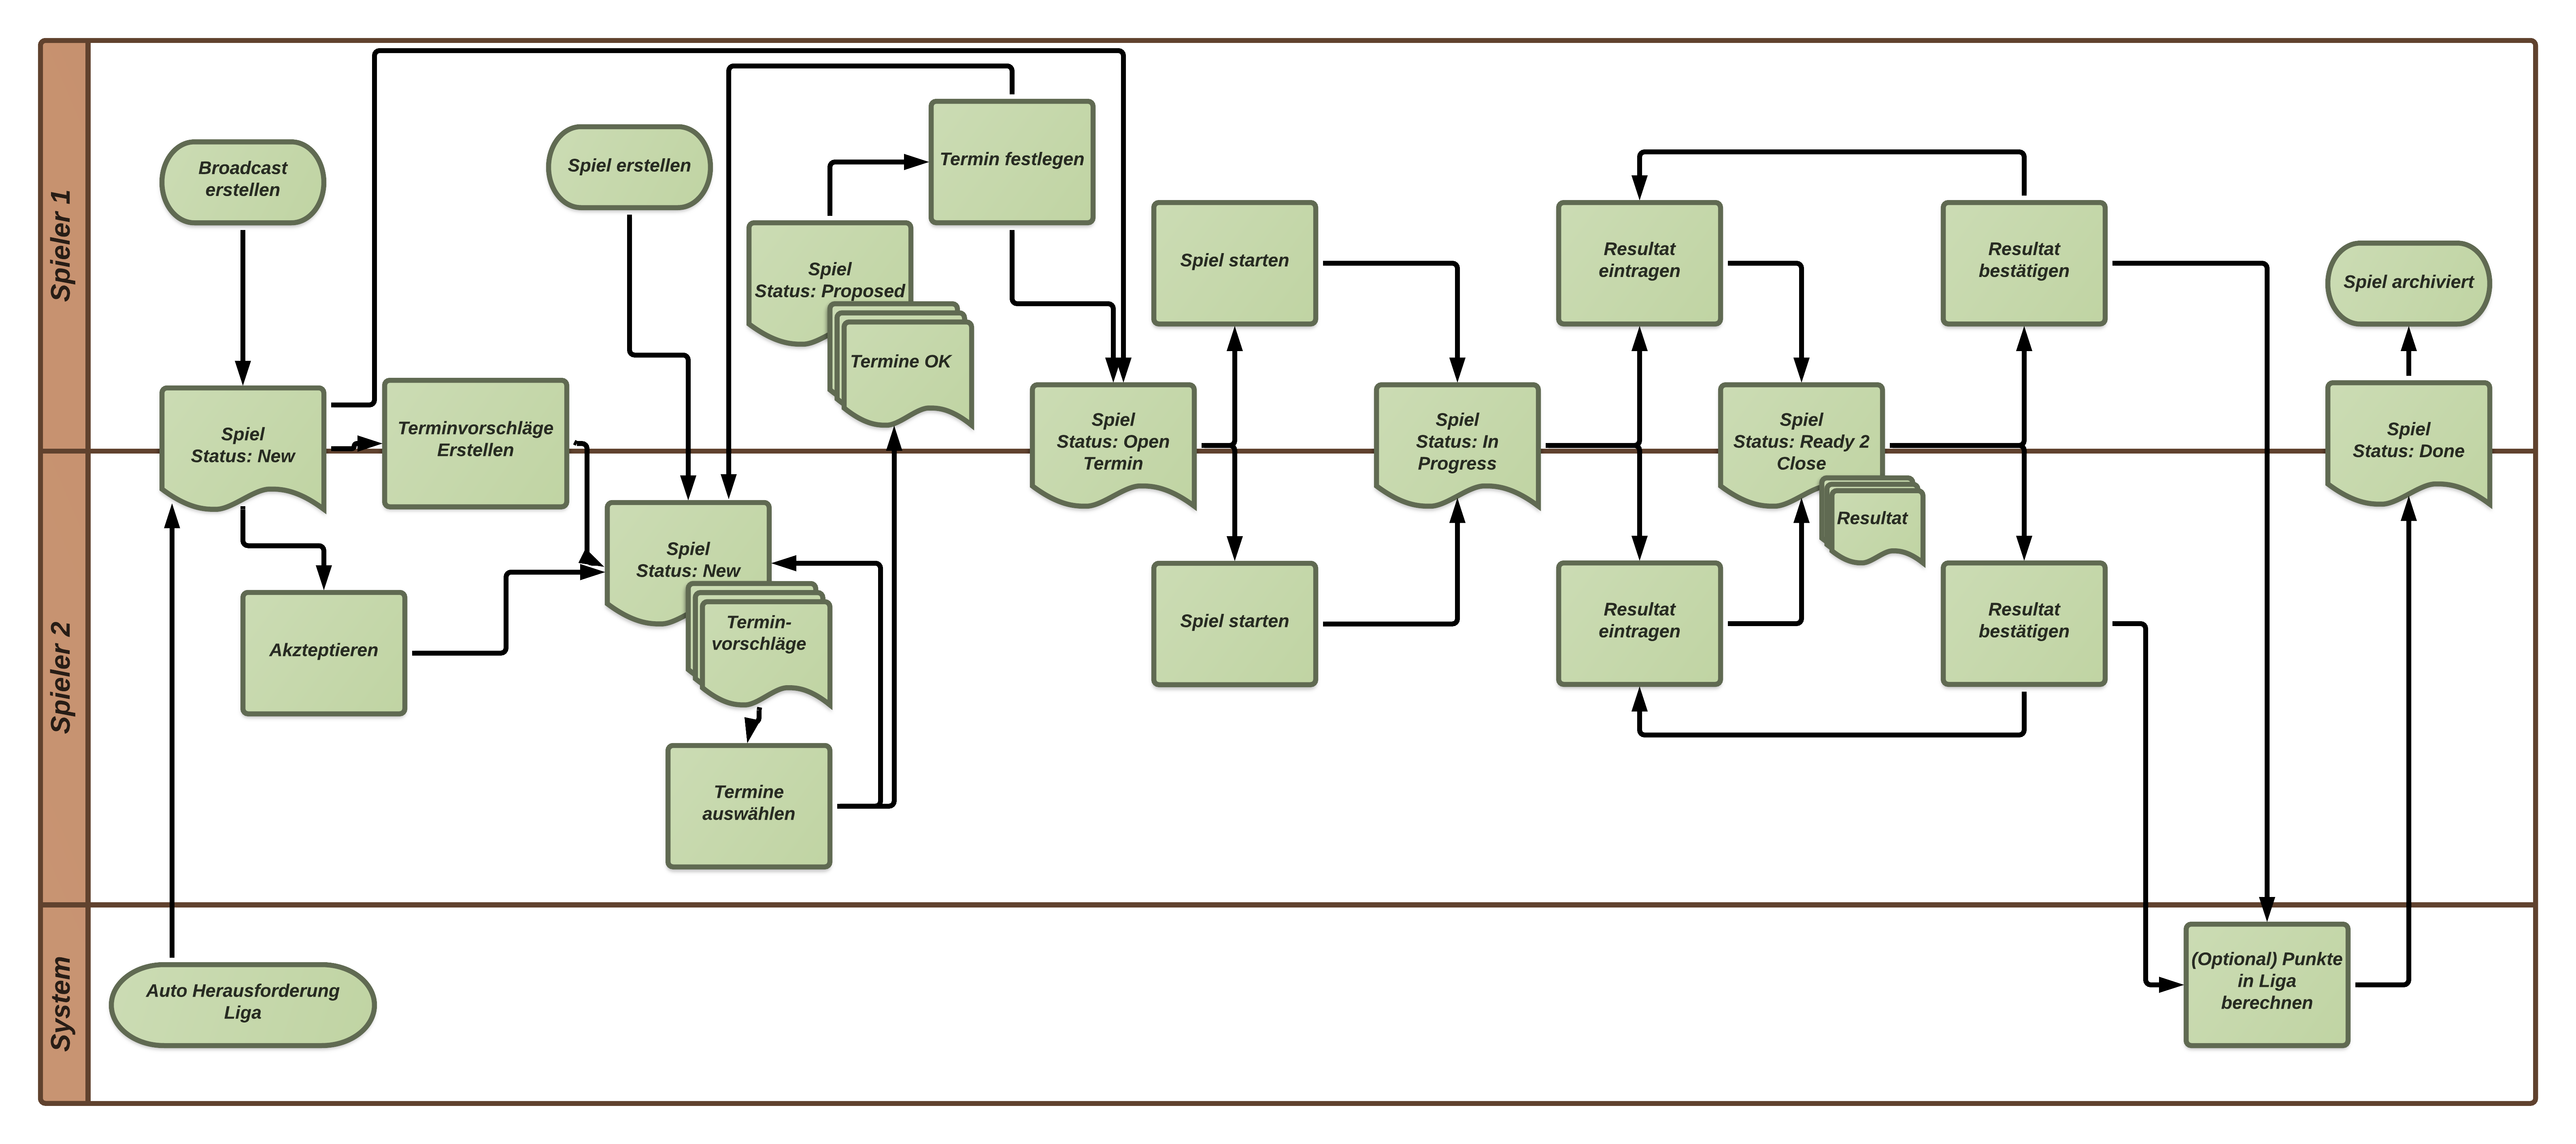
\includegraphics[width=1.3\textwidth]{Graphics/match_workflow.png}
	\caption{Spiel Workflow}
	\label{MatchWorkflow}
\end{figure}
\end{landscape}

Der Workflow wird �ber drei verschiedene F�lle gestartet: 
\begin{itemize}
	\itemsep -0.5em
	\item Das System erstellt Auto-Herausforderungen f�r die Liga
	\item Der User erstellt ein Broadcast Spiel
	\item Der User erstellt ein regul�res spiel.
	
	\end{itemize}
	
Wenn der User ein \textbf{regul�res Spiel} erstellt, sind beide Spieler, sowie Terminvorschl�ge schon definiert. Es folgt die Aktion \grqq Termin ausw�hlen\grqq.

Erstellt der User ein \textbf{broadcast Spiel}, hat das Spiel den Status \grqq New\grqq, jedoch noch keinen zweiten Spieler definiert. Zus�tzlich werden keine Terminvorschl�ge ausgef�llt, sondern einen fixen Termin. Akzeptiert jemand den Broadcast wird der zweite Spieler eingetragen und der Status �ndert sich direkt auf Open.
 
Sind User in einer Liga, erstellt die \textbf{Liga eine Herausforderung}. Das Spiel enth�lt kein Court und keine Terminvorschl�ge. Der User muss nun Terminvorschl�ge ausf�llen und ein Court definieren. 

Anschliessend haben alle Use Cases den gleichen Workflow. Ist das Spiel und der Termin definiert. Geht der Status des Spiels zu \grqq Open\grqq . Danach kann von beiden Spielern der Status auf \grqq In progress\grqq gesetzt werden. Beide k�nnen ein Resultat eintragen. Der jeweil andere Spieler best�tigt anschliessend das Resultat. Bei der Best�tigung des Resultats wird das Spiel archiviert und optional die Rangliste der Liga aktualisiert.
\newpage

\section{User}
\subsection{Freunde System}
\begin{figure}[ht]
	\centering
	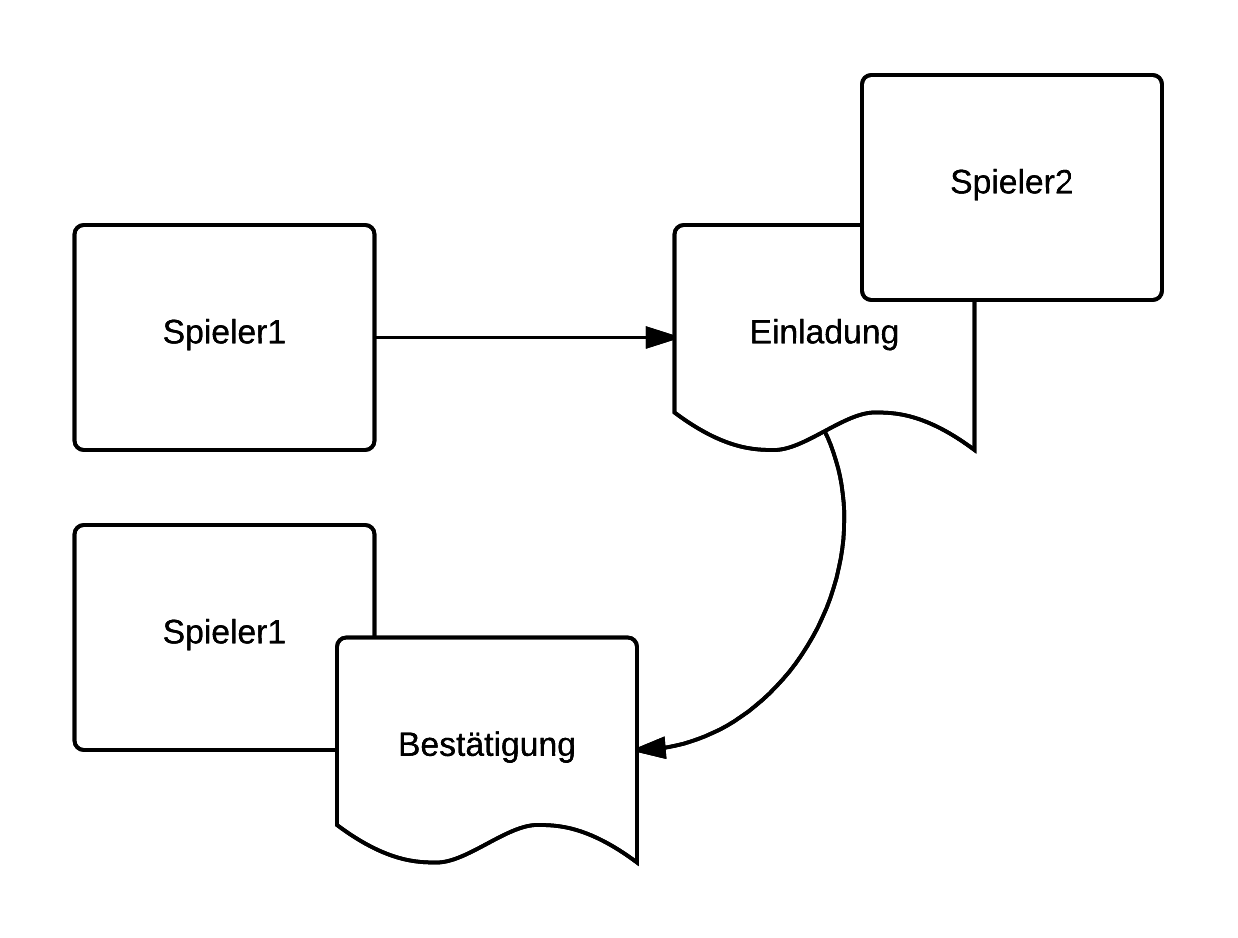
\includegraphics[width=0.7\textwidth]{Graphics/friendworkflow.png}
	\caption{Freunde Workflow}
	\label{FriendWorkflow}
\end{figure}
\FloatBarrier
Spieler1 sendet eine Einladung zur Freundschaft an Spieler 2. Diese Einladung ist eine Liste bei Spieler2 sowie bei Spieler1:
\begin{lstlisting}
friendrequests: [{
		type: Schema.ObjectId,
		ref: "User"
	}],
\end{lstlisting}
Bei der Best�tigung der Einladung tr�gt sich Spieler2 sowie Spieler1 das User-Objekt von dem friendrequests Feld in das friends Feld:
\begin{lstlisting}
friends: [{
		type: Schema.ObjectId,
		ref: "User"
	}],
\end{lstlisting}
% !TeX spellcheck = de_CH
\chapter{Test}
\section{Unit Tests}
Der MEAN Stack bietet ein Framework direkt an. Es wird unterschieden zwischen dem Client Test Framework und dem Server Test Framework.

Als Client Test Framework wird Karma --- ein Framework, um AngularJS zu testen --- verwendet. F�r jeden Controller werden die verschiedenen Methoden getestet.  Als Beispiel testet dieser Test, ob die find()-Methode gew�nscht funktioniert:
\begin{lstlisting}
it('$scope.find() should create an array with at least one Court object fetched from XHR', inject(function(Courts) {
	// Create sample Court using the Courts service
	var sampleCourt = new Courts({
		'name':'Vitis','address':'Vitis','contact':'000000000','sports':['Squash','Tennis','Badminton','Tabletennis']
	});

	// Create a sample Courts array that includes the new Court
	var sampleCourts = [sampleCourt];

	// Set GET response
	$httpBackend.expectGET('courts').respond(sampleCourts);

	// Run controller functionality
	scope.find();
	$httpBackend.flush();

	// Test scope value
	expect(scope.courts).toEqualData(sampleCourts);
}));
\end{lstlisting}

Zuerst wird ein Beispiel-Court-Objekt erstellt (Zeile 3--5). Auf Zeile 11 wird ein Mock-Objekt erstellt, das den API Call /courts abf�ngt, und das Beispiel-Court zur�cksendet. Anschliessend wird (Zeile 14) die Methode aufgerufen und auf Zeile 18 die Antwort mit dem Anfang verglichen. Sind die Daten gleich, ist der Test f�r die Methode gegl�ckt.

Als Server Test Framework wird Mocha --- eine NodeJS/ExpressJS Testsuite verwendet. Models sowie Controller werden hier getestet. 

Als Beispiel testet dieser Code, ob die Datenfelder richtig spezifiziert sind, und verschiedene Save-Funktionen funktionieren oder einen Fehler zur�ckgeben:
\begin{lstlisting}
describe('Method Save', function() {
	it('should be able to save without problems', function(done) {
		return court.save(function(err) {
			should.not.exist(err);
			done();
		});
	});

	it('should be able to show an error when try to save without name', function(done) { 
		court.name = '';

		return court.save(function(err) {
			should.exist(err);
			done();
		});
	});
	it('should be able to show an error when try to save without coordinates', function(done) {
		court.lat = '';

		return court.save(function(err) {
			should.exist(err);
			done();
		});
	});
});
\end{lstlisting}
Der erste Test pr�ft, ob ein valides (zuvor erstelltes) Court-Objekt  problemlos gespeichert werden kann. Daf�r wird die court.save() Funktion aufgerufen und gepr�ft, ob es einen Error gibt.

Anschliessend (ab Zeile 9) wird der Name oder die Koordinaten (ab Zeile 17) gel�scht, was nicht zul�ssig ist. Das Resultat bei dem Speichern des Objekt sollte ein Error sein. Ist dem so, ist der Test erfolgreich.

Bei den Controller Tests wird die Applikation in der Test-Umgebung gestartet. Verschiedene Objekte werden bei Teststart in die Test-Datenbank eingef�gt:
\begin{lstlisting}
....
beforeEach(function(done) {
		// Create user credentials
		credentials = {
			username: 'username',
			password: 'password'
		};

		// Create a new user
		user = new User({
			firstName: 'Full',
			lastName: 'Name',
			displayName: 'Full Name',
			email: 'test@test.com',
			username: credentials.username,
			password: credentials.password,
			provider: 'local'
		});

		// Save a user to the test db and create new Court
		user.save(function() {
....
\end{lstlisting}
Anschliessend wird die Applikation mit verschieden Requests angesprochen und die Response auf Validit�t �berpr�ft:
\begin{lstlisting}
it('should not be able to save Court instance if not logged in', function(done) {
		agent.post('/courts')
			.send(court)
			.expect(401)
			.end(function(courtSaveErr, courtSaveRes) {
				// Call the assertion callback
				done(courtSaveErr);
			});
	});
\end{lstlisting}
In diesem Beispiel wird versucht ein Court anzulegen, ohne vorher einzuloggen. Ein Access Denied Fehler muss von der API zur�ckgesendet werden (siehe Zeile 4).

\section{System Tests}
Zus�tzlich zu den Unit Tests werden die Anforderungen manuell getestet mithilfe eines Systemtests. Zuerst werden Testf�lle f�r Anforderungen erstellt, diese ausgef�hrt und das erwartete Ergebnis mit dem tats�chlichen verglichen. 
\newpage
\subsection{Testf�lle}
\begin{center}
	\tabulinesep = 1mm
	\begin{longtabu} to \linewidth [m]{|[2pt]p{3cm}|[2pt]X[1, m , l]|[2pt]}
		\arrayrulecolor{white}	
		\tabucline[2pt]{-}
		\textcolor{white}{\textbf{\cellcolor{airforceblue}TE0.01}}  &   
		\textcolor{white}{\textbf{\cellcolor{airforceblue}Erfolgreiche Anmeldung an das System }}
		\tabularnewline
		\tabucline[2pt]{-}
		\textcolor{white}{\textbf{\cellcolor{airforceblue}Beschreibung}} &  
		\cellcolor{testblau}{Dieser Test pr�ft, ob eine Anmeldung an das System funktioniert mit g�ltigen Anmeldedaten. }
		\tabularnewline
		\tabucline[2pt]{-}
		\textcolor{white}{\textbf{\cellcolor{airforceblue}Version}} &
		\cellcolor{testblau} 1.0
		\tabularnewline
		\tabucline[2pt]{-}
		\textcolor{white}{\textbf{\cellcolor{airforceblue}Getestete Anforderung}} &
		\cellcolor{testblau} REQ0.01 --- Anmeldung an das System
		\tabularnewline
		\tabucline[2pt]{-}
		\textcolor{white}{\textbf{\cellcolor{airforceblue}Testschritte }} &
		\cellcolor{testblau}
		\begin{enumerate}
		\itemsep -0.4em
			\item Navigieren zur Anmeldeseite (webserver/signin)
			\item Eingeben von g�ltigen Anmeldedaten
		\end{enumerate}
		\tabularnewline
		\tabucline[2pt]{-}
		\textcolor{white}{\textbf{\cellcolor{airforceblue}Erwartetes Resultat}} &
		\cellcolor{testblau}	
		Erfolgreicher Login, Weiterleitung zur Startseite. 
	\end{longtabu}
\end{center}
\begin{center}
	\tabulinesep = 1mm
	\begin{longtabu} to \linewidth [m]{|[2pt]p{3cm}|[2pt]X[1, m , l]|[2pt]}
		\arrayrulecolor{white}	
		\tabucline[2pt]{-}
		\textcolor{white}{\textbf{\cellcolor{airforceblue}TE0.02}}  &   
		\textcolor{white}{\textbf{\cellcolor{airforceblue}Fehlgeschlagene Anmeldung an das System }}
		\tabularnewline
		\tabucline[2pt]{-}
		\textcolor{white}{\textbf{\cellcolor{airforceblue}Beschreibung}} &  
		\cellcolor{testblau}{Dieser Test pr�ft, ob eine Anmeldung an das System fehlschl�gt mit falschen Anmeldedaten }
		\tabularnewline
		\tabucline[2pt]{-}
		\textcolor{white}{\textbf{\cellcolor{airforceblue}Version}} &
		\cellcolor{testblau} 1.0
		\tabularnewline
		\tabucline[2pt]{-}
		\textcolor{white}{\textbf{\cellcolor{airforceblue}Getestete Anforderung}} &
		\cellcolor{testblau} REQ0.01 --- Anmeldung an das System
		\tabularnewline
		\tabucline[2pt]{-}
		\textcolor{white}{\textbf{\cellcolor{airforceblue}Testschritte }} &
		\cellcolor{testblau}
		\begin{enumerate}
		\itemsep -0.4em
			\item Navigieren zur Anmeldeseite (webserver/signin)
			\item Eingeben von ung�ltigen Anmeldedaten
		\end{enumerate}
		\tabularnewline
		\tabucline[2pt]{-}
		\textcolor{white}{\textbf{\cellcolor{airforceblue}Erwartetes Resultat}} &
		\cellcolor{testblau}	
		Fehlgeschlagener Login, Fehlermeldung (z.B. Wrong Username/Password)
	\end{longtabu}
\end{center}
\begin{center}
	\tabulinesep = 1mm
	\begin{longtabu} to \linewidth [m]{|[2pt]p{3cm}|[2pt]X[1, m , l]|[2pt]}
		\arrayrulecolor{white}	
		\tabucline[2pt]{-}
		\textcolor{white}{\textbf{\cellcolor{airforceblue}TE0.03}}  &   
		\textcolor{white}{\textbf{\cellcolor{airforceblue}Erfolgreiche Anmeldung an das System mittels OAuth}}
		\tabularnewline
		\tabucline[2pt]{-}
		\textcolor{white}{\textbf{\cellcolor{airforceblue}Beschreibung}} &  
		\cellcolor{testblau}{Dieser Test pr�ft, ob eine Anmeldung an das System mit OAuth funktioniert. }
		\tabularnewline
		\tabucline[2pt]{-}
		\textcolor{white}{\textbf{\cellcolor{airforceblue}Version}} &
		\cellcolor{testblau} 1.0
		\tabularnewline
		\tabucline[2pt]{-}
		\textcolor{white}{\textbf{\cellcolor{airforceblue}Getestete Anforderung}} &
		\cellcolor{testblau} REQ0.03 --- Authentisierung �ber OAuth
		\tabularnewline
		\tabucline[2pt]{-}
		\textcolor{white}{\textbf{\cellcolor{airforceblue}Testschritte }} &
		\cellcolor{testblau}
		\begin{enumerate}
		\itemsep -0.4em
			\item Navigieren zur Anmeldeseite (webserver/signin)
			\item Auf das OAuth Symbol von Google klicken
			\item Bei Google anmelden
			\item Autorisierung (wenn noch nicht gemacht) freigeben
		\end{enumerate}
		\tabularnewline
		\tabucline[2pt]{-}
		\textcolor{white}{\textbf{\cellcolor{airforceblue}Erwartetes Resultat}} &
		\cellcolor{testblau}	
		Erfolgreicher Login, Weiterleitung zur Startseite.
	\end{longtabu}
\end{center}
\begin{center}
	\tabulinesep = 1mm
	\begin{longtabu} to \linewidth [m]{|[2pt]p{3cm}|[2pt]X[1, m , l]|[2pt]}
		\arrayrulecolor{white}	
		\tabucline[2pt]{-}
		\textcolor{white}{\textbf{\cellcolor{airforceblue}TE0.04}}  &   
		\textcolor{white}{\textbf{\cellcolor{airforceblue}Erfolgreiche Registrierung mit dem System}}
		\tabularnewline
		\tabucline[2pt]{-}
		\textcolor{white}{\textbf{\cellcolor{airforceblue}Beschreibung}} &  
		\cellcolor{testblau}{Dieser Test pr�ft, ob die Registrierung mit einem validen User funktioniert }
		\tabularnewline
		\tabucline[2pt]{-}
		\textcolor{white}{\textbf{\cellcolor{airforceblue}Version}} &
		\cellcolor{testblau} 1.0
		\tabularnewline
		\tabucline[2pt]{-}
		\textcolor{white}{\textbf{\cellcolor{airforceblue}Getestete Anforderung}} &
		\cellcolor{testblau} REQ0.02 --- Registrierung eines Users mit dem System
		\tabularnewline
		\tabucline[2pt]{-}
		\textcolor{white}{\textbf{\cellcolor{airforceblue}Testschritte }} &
		\cellcolor{testblau}
		\begin{enumerate}
		\itemsep -0.4em
			\item Navigieren zur Registrierungsseite (webserver/signup)
			\item Einen neuen validen User registrieren

		\end{enumerate}
		\tabularnewline
		\tabucline[2pt]{-}
		\textcolor{white}{\textbf{\cellcolor{airforceblue}Erwartetes Resultat}} &
		\cellcolor{testblau}	
		Erfolgreiche Registrierung, Weiterleitung zur Profil- oder Startseite.
	\end{longtabu}
\end{center}
\begin{center}
	\tabulinesep = 1mm
	\begin{longtabu} to \linewidth [m]{|[2pt]p{3cm}|[2pt]X[1, m , l]|[2pt]}
		\arrayrulecolor{white}	
		\tabucline[2pt]{-}
		\textcolor{white}{\textbf{\cellcolor{airforceblue}TE0.05}}  &   
		\textcolor{white}{\textbf{\cellcolor{airforceblue}Gleiche E-Mail bei Registrierung}}
		\tabularnewline
		\tabucline[2pt]{-}
		\textcolor{white}{\textbf{\cellcolor{airforceblue}Beschreibung}} &  
		\cellcolor{testblau}{Dieser Test pr�ft, ob die Registrierung mit einem schon existierenden User  einen Fehler gibt }
		\tabularnewline
		\tabucline[2pt]{-}
		\textcolor{white}{\textbf{\cellcolor{airforceblue}Version}} &
		\cellcolor{testblau} 1.0
		\tabularnewline
		\tabucline[2pt]{-}
		\textcolor{white}{\textbf{\cellcolor{airforceblue}Getestete Anforderung}} &
		\cellcolor{testblau} REQ0.02 - Registrierung eines Users mit dem System
		\tabularnewline
		\tabucline[2pt]{-}
		\textcolor{white}{\textbf{\cellcolor{airforceblue}Testschritte }} &
		\cellcolor{testblau}
		\begin{enumerate}
		\itemsep -0.4em
			\item Navigieren zur Registrierungsseite (webserver/signup)
			\item Einen existierenden User mit gleicher E-Mail registrieren
		\end{enumerate}
		\tabularnewline
		\tabucline[2pt]{-}
		\textcolor{white}{\textbf{\cellcolor{airforceblue}Erwartetes Resultat}} &
		\cellcolor{testblau}	
		Fehlermeldung, der User ist vorhanden
	\end{longtabu}
\end{center}
\begin{center}
	\tabulinesep = 1mm
	\begin{longtabu} to \linewidth [m]{|[2pt]p{3cm}|[2pt]X[1, m , l]|[2pt]}
		\arrayrulecolor{white}	
		\tabucline[2pt]{-}
		\textcolor{white}{\textbf{\cellcolor{airforceblue}TE1.01}}  &   
		\textcolor{white}{\textbf{\cellcolor{airforceblue}User registriert sich und verl�sst  Racket-Sportzentrum}}
		\tabularnewline
		\tabucline[2pt]{-}
		\textcolor{white}{\textbf{\cellcolor{airforceblue}Beschreibung}} &  
		\cellcolor{testblau}{Der User w�hlt ein Racket-Sportzentrum aus und registriert sich darin }
		\tabularnewline
		\tabucline[2pt]{-}
		\textcolor{white}{\textbf{\cellcolor{airforceblue}Version}} &
		\cellcolor{testblau} 1.0
		\tabularnewline
		\tabucline[2pt]{-}
		\textcolor{white}{\textbf{\cellcolor{airforceblue}Getestete Anforderung}} &
		\cellcolor{testblau} REQ0.02 --- Registrierung eines Users mit dem System
		\tabularnewline
		\tabucline[2pt]{-}
		\textcolor{white}{\textbf{\cellcolor{airforceblue}Testschritte }} &
		\cellcolor{testblau}
		\begin{enumerate}
		\itemsep -0.4em
			\item Navigieren zur Courtsite (webserver/courts)
			\item Ein Racket-Sportzentrum ausw�hlen.
			\item Auf  \guillemotleft Ich will mitspielen\guillemotright {} dr�cken, um sich mit dem Racket-Sportzentrum zu registrieren.
			\item Auf \guillemotleft Ich will nicht mehr mitspielen\guillemotright {}  dr�cken, um sich auszutragen.
		\end{enumerate}
		\tabularnewline
		\tabucline[2pt]{-}
		\textcolor{white}{\textbf{\cellcolor{airforceblue}Erwartetes Resultat}} &
		\cellcolor{testblau}	
		Nach Schritt 3 muss der User in der Liste des Racket-Sportzentrums auftauchen. Nach Schritt 4 muss der User aus der Liste verschwinden
	\end{longtabu}
\end{center}
\begin{center}
	\tabulinesep = 1mm
	\begin{longtabu} to \linewidth [m]{|[2pt]p{3cm}|[2pt]X[1, m , l]|[2pt]}
		\arrayrulecolor{white}	
		\tabucline[2pt]{-}
		\textcolor{white}{\textbf{\cellcolor{airforceblue}TE1.02}}  &   
		\textcolor{white}{\textbf{\cellcolor{airforceblue}Details zu Spielern}}
		\tabularnewline
		\tabucline[2pt]{-}
		\textcolor{white}{\textbf{\cellcolor{airforceblue}Beschreibung}} &  
		\cellcolor{testblau}{Der Spieler kann Details �ber sich preisgeben. Es gibt eine Seite, auf der er die Informationen �ber ein Formular eintragen kann.}
		\tabularnewline
		\tabucline[2pt]{-}
		\textcolor{white}{\textbf{\cellcolor{airforceblue}Version}} &
		\cellcolor{testblau} 1.0
		\tabularnewline
		\tabucline[2pt]{-}
		\textcolor{white}{\textbf{\cellcolor{airforceblue}Getestete Anforderung}} &
		\cellcolor{testblau} REQ1.01 --- Zuteilung von User zu Racket-Sportzentren
		\tabularnewline
		\tabucline[2pt]{-}
		\textcolor{white}{\textbf{\cellcolor{airforceblue}Testschritte }} &
		\cellcolor{testblau}
		\begin{enumerate}
		\itemsep -0.4em
			\item Navigieren zur Profilseite (webserver/profile)
			\item Informationen �ber das Formular eintragen
			\item Formular abschicken
		
		\end{enumerate}
		\tabularnewline
		\tabucline[2pt]{-}
		\textcolor{white}{\textbf{\cellcolor{airforceblue}Erwartetes Resultat}} &
		\cellcolor{testblau}	
		Informationen nach einem Reload immer noch auf der Profilseite vorhanden.
	\end{longtabu}
\end{center}
\begin{center}
	\tabulinesep = 1mm
	\begin{longtabu} to \linewidth [m]{|[2pt]p{3cm}|[2pt]X[1, m , l]|[2pt]}
		\arrayrulecolor{white}	
		\tabucline[2pt]{-}
		\textcolor{white}{\textbf{\cellcolor{airforceblue}TE1.03}}  &   
		\textcolor{white}{\textbf{\cellcolor{airforceblue}Friend System - Freund einladen}}
		\tabularnewline
		\tabucline[2pt]{-}
		\textcolor{white}{\textbf{\cellcolor{airforceblue}Beschreibung}} &  
		\cellcolor{testblau}{Spieler 1 l�dt Spieler 2 ein, ein Freund zu werden. Spieler 2 sieht die Einladung und kann sie annehmen oder ablehnen.}
		\tabularnewline
		\tabucline[2pt]{-}
		\textcolor{white}{\textbf{\cellcolor{airforceblue}Version}} &
		\cellcolor{testblau} 1.0
		\tabularnewline
		\tabucline[2pt]{-}
		\textcolor{white}{\textbf{\cellcolor{airforceblue}Getestete Anforderung}} &
		\cellcolor{testblau} REQ1.03 --- Friend System
		\tabularnewline
		\tabucline[2pt]{-}
		\textcolor{white}{\textbf{\cellcolor{airforceblue}Testschritte }} &
		\cellcolor{testblau}
		\begin{enumerate}
		\itemsep -0.4em
			\item Navigieren zur Freundeseite (webserver/friends)
			\item Name von Spieler 2 in Formular eingeben
			\item Einladung senden
		\end{enumerate}
		\tabularnewline
		\tabucline[2pt]{-}
		\textcolor{white}{\textbf{\cellcolor{airforceblue}Erwartetes Resultat}} &
		\cellcolor{testblau}	
		Spieler 2 sieht eine Einladung von Spieler 1
	\end{longtabu}
\end{center}
\begin{center}
	\tabulinesep = 1mm
	\begin{longtabu} to \linewidth [m]{|[2pt]p{3cm}|[2pt]X[1, m , l]|[2pt]}
		\arrayrulecolor{white}	
		\tabucline[2pt]{-}
		\textcolor{white}{\textbf{\cellcolor{airforceblue}TE1.04}}  &   
		\textcolor{white}{\textbf{\cellcolor{airforceblue}Friend System --- Einladung annehmen}}
		\tabularnewline
		\tabucline[2pt]{-}
		\textcolor{white}{\textbf{\cellcolor{airforceblue}Beschreibung}} &  
		\cellcolor{testblau}{Spieler 2 nimmt die Einladung an. Beide Spieler sehen sich nun als Freunde}
		\tabularnewline
		\tabucline[2pt]{-}
		\textcolor{white}{\textbf{\cellcolor{airforceblue}Version}} &
		\cellcolor{testblau} 1.0
		\tabularnewline
		\tabucline[2pt]{-}
		\textcolor{white}{\textbf{\cellcolor{airforceblue}Getestete Anforderung}} &
		\cellcolor{testblau} REQ1.03 --- Friend System
		\tabularnewline
		\tabucline[2pt]{-}
		\textcolor{white}{\textbf{\cellcolor{airforceblue}Testschritte }} &
		\cellcolor{testblau}
		\begin{enumerate}
		\itemsep -0.4em
			\item Navigieren zur Freundeseite (webserver/friends)
			\item Einladung von Spieler 1 annehmen
		\end{enumerate}
		\tabularnewline
		\tabucline[2pt]{-}
		\textcolor{white}{\textbf{\cellcolor{airforceblue}Erwartetes Resultat}} &
		\cellcolor{testblau}	
		Beide sehen sich als Freunde auf der Freundeseite.
	\end{longtabu}
\end{center}
\begin{center}
	\tabulinesep = 1mm
	\begin{longtabu} to \linewidth [m]{|[2pt]p{3cm}|[2pt]X[1, m , l]|[2pt]}
		\arrayrulecolor{white}	
		\tabucline[2pt]{-}
		\textcolor{white}{\textbf{\cellcolor{airforceblue}TE1.05}}  &   
		\textcolor{white}{\textbf{\cellcolor{airforceblue}Friend System --- Einladung ablehnen}}
		\tabularnewline
		\tabucline[2pt]{-}
		\textcolor{white}{\textbf{\cellcolor{airforceblue}Beschreibung}} &  
		\cellcolor{testblau}{Spieler 2 lehnt die Einladung ab. Beide Spieler sehen sich nicht als freunde}
		\tabularnewline
		\tabucline[2pt]{-}
		\textcolor{white}{\textbf{\cellcolor{airforceblue}Version}} &
		\cellcolor{testblau} 1.0
		\tabularnewline
		\tabucline[2pt]{-}
		\textcolor{white}{\textbf{\cellcolor{airforceblue}Getestete Anforderung}} &
		\cellcolor{testblau} REQ1.03 --- Friend System
		\tabularnewline
		\tabucline[2pt]{-}
		\textcolor{white}{\textbf{\cellcolor{airforceblue}Testschritte }} &
		\cellcolor{testblau}
		\begin{enumerate}
		\itemsep -0.4em
			\item Navigieren zur Freundeseite (webserver/friends)
			\item Einladung von Spieler 1 ablehnen
		\end{enumerate}
		\tabularnewline
		\tabucline[2pt]{-}
		\textcolor{white}{\textbf{\cellcolor{airforceblue}Erwartetes Resultat}} &
		\cellcolor{testblau}	
		Beide sehen sich nicht als Freunde auf der Freundeseite.
	\end{longtabu}
\end{center}
\begin{center}
	\tabulinesep = 1mm
	\begin{longtabu} to \linewidth [m]{|[2pt]p{3cm}|[2pt]X[1, m , l]|[2pt]}
		\arrayrulecolor{white}	
		\tabucline[2pt]{-}
		\textcolor{white}{\textbf{\cellcolor{airforceblue}TE1.06}}  &   
		\textcolor{white}{\textbf{\cellcolor{airforceblue}Friend System --- nicht vorhandenen User einladen}}
		\tabularnewline
		\tabucline[2pt]{-}
		\textcolor{white}{\textbf{\cellcolor{airforceblue}Beschreibung}} &  
		\cellcolor{testblau}{Spieler 1 l�dt einen nicht vorhandenen User ein.}
		\tabularnewline
		\tabucline[2pt]{-}
		\textcolor{white}{\textbf{\cellcolor{airforceblue}Version}} &
		\cellcolor{testblau} 1.0
		\tabularnewline
		\tabucline[2pt]{-}
		\textcolor{white}{\textbf{\cellcolor{airforceblue}Getestete Anforderung}} &
		\cellcolor{testblau} REQ1.03 --- Friend System
		\tabularnewline
		\tabucline[2pt]{-}
		\textcolor{white}{\textbf{\cellcolor{airforceblue}Testschritte }} &
		\cellcolor{testblau}
		\begin{enumerate}
		\itemsep -0.4em
			\item Navigieren zur Freundeseite (webserver/friends)
			\item Einladung an Username senden, welcher nicht existiert
		\end{enumerate}
		\tabularnewline
		\tabucline[2pt]{-}
		\textcolor{white}{\textbf{\cellcolor{airforceblue}Erwartetes Resultat}} &
		\cellcolor{testblau}	
		Ein Fehler wird zur�ckgegeben, dass der User nicht gefunden wurde.
	\end{longtabu}
\end{center}
\begin{center}
	\tabulinesep = 1mm
	\begin{longtabu} to \linewidth [m]{|[2pt]p{3cm}|[2pt]X[1, m , l]|[2pt]}
		\arrayrulecolor{white}	
		\tabucline[2pt]{-}
		\textcolor{white}{\textbf{\cellcolor{airforceblue}TE2.01}}  &   
		\textcolor{white}{\textbf{\cellcolor{airforceblue}Spiel mit Terminvorschlag erstellen}}
		\tabularnewline
		\tabucline[2pt]{-}
		\textcolor{white}{\textbf{\cellcolor{airforceblue}Beschreibung}} &  
		\cellcolor{testblau}{Ein Spieler erstellt ein Spiel.}
		\tabularnewline
		\tabucline[2pt]{-}
		\textcolor{white}{\textbf{\cellcolor{airforceblue}Version}} &
		\cellcolor{testblau} 1.0
		\tabularnewline
		\tabucline[2pt]{-}
		\textcolor{white}{\textbf{\cellcolor{airforceblue}Getestete Anforderung}} &
		\cellcolor{testblau} 
		\begin{itemize}
		\item REQ2.01 --- Spiel erstellen
		\item REQ2.02 --- Spiel Terminvorschl�ge erstellen
		\end{itemize}
		\tabularnewline
		\tabucline[2pt]{-}
		\textcolor{white}{\textbf{\cellcolor{airforceblue}Testschritte }} &
		\cellcolor{testblau}
		\begin{enumerate}
		\itemsep -0.4em
			\item Navigieren zur Spieleseite (webserver/matches)
			\item Erstellen eines Spiels
			\item Alle Felder einf�llen , inklusive Terminvorschl�ge
			\item Spiel abschicken
		\end{enumerate}
		\tabularnewline
		\tabucline[2pt]{-}
		\textcolor{white}{\textbf{\cellcolor{airforceblue}Erwartetes Resultat}} &
		\cellcolor{testblau}	
		Spieler 2 sollte nun das Spiel sehen
	\end{longtabu}
\end{center}
\begin{center}
	\tabulinesep = 1mm
	\begin{longtabu} to \linewidth [m]{|[2pt]p{3cm}|[2pt]X[1, m , l]|[2pt]}
		\arrayrulecolor{white}	
		\tabucline[2pt]{-}
		\textcolor{white}{\textbf{\cellcolor{airforceblue}TE2.02}}  &   
		\textcolor{white}{\textbf{\cellcolor{airforceblue}Nicht valides Spiel erstellen}}
		\tabularnewline
		\tabucline[2pt]{-}
		\textcolor{white}{\textbf{\cellcolor{airforceblue}Beschreibung}} &  
		\cellcolor{testblau}{Ein Spieler erstellt ein Spiel}
		\tabularnewline
		\tabucline[2pt]{-}
		\textcolor{white}{\textbf{\cellcolor{airforceblue}Version}} &
		\cellcolor{testblau} 1.0
		\tabularnewline
		\tabucline[2pt]{-}
		\textcolor{white}{\textbf{\cellcolor{airforceblue}Getestete Anforderung}} &
		\cellcolor{testblau} 
		\begin{itemize}
		\item REQ2.01 --- Spiel erstellen
		\item REQ2.02 --- Spiel Terminvorschl�ge erstellen
		\end{itemize}
		\tabularnewline
		\tabucline[2pt]{-}
		\textcolor{white}{\textbf{\cellcolor{airforceblue}Testschritte }} &
		\cellcolor{testblau}
		\begin{enumerate}
		\itemsep -0.4em
			\item Navigieren zur Spieleseite (webserver/matches)
			\item Erstellen eines Spiels
			\item Kein Sport ausf�llen
			\item Spiel abschicken
		\end{enumerate}
		\tabularnewline
		\tabucline[2pt]{-}
		\textcolor{white}{\textbf{\cellcolor{airforceblue}Erwartetes Resultat}} &
		\cellcolor{testblau}	
		Beim abschicken sollte ein Fehler erscheinen, dass das Spiel nicht vollst�ndig ausgef�llt wurde.
	\end{longtabu}
\end{center}

\begin{center}
	\tabulinesep = 1mm
	\begin{longtabu} to \linewidth [m]{|[2pt]p{3cm}|[2pt]X[1, m , l]|[2pt]}
		\arrayrulecolor{white}	
		\tabucline[2pt]{-}
		\textcolor{white}{\textbf{\cellcolor{airforceblue}TE2.03}}  &   
		\textcolor{white}{\textbf{\cellcolor{airforceblue}Spiel Terminvorschlag annehmen}}
		\tabularnewline
		\tabucline[2pt]{-}
		\textcolor{white}{\textbf{\cellcolor{airforceblue}Beschreibung}} &  
		\cellcolor{testblau}{Ein Spieler nimmt ein Spiel an.}
		\tabularnewline
		\tabucline[2pt]{-}
		\textcolor{white}{\textbf{\cellcolor{airforceblue}Version}} &
		\cellcolor{testblau} 1.0
		\tabularnewline
		\tabucline[2pt]{-}
		\textcolor{white}{\textbf{\cellcolor{airforceblue}Getestete Anforderung}} &
		\cellcolor{testblau} 
		 REQ2.03 --- Spiel Terminvorschl�ge annehmen und ablehnen
		\tabularnewline
		\tabucline[2pt]{-}
		\textcolor{white}{\textbf{\cellcolor{airforceblue}Testschritte }} &
		\cellcolor{testblau}
		\begin{enumerate}
		\itemsep -0.4em
			\item Navigieren zur Spieleseite (webserver/matches)
			\item Einen Spielvorschlag ausw�hlen
			\item Einen Terminvorschlag w�hlen
			\item Spiel abschicken
		\end{enumerate}
		\tabularnewline
		\tabucline[2pt]{-}
		\textcolor{white}{\textbf{\cellcolor{airforceblue}Erwartetes Resultat}} &
		\cellcolor{testblau}	
		Der User sieht das Spiel nicht mehr, der andere Spieler kann nun den Vorschlag best�tigen
	\end{longtabu}
\end{center}
\begin{center}
	\tabulinesep = 1mm
	\begin{longtabu} to \linewidth [m]{|[2pt]p{3cm}|[2pt]X[1, m , l]|[2pt]}
		\arrayrulecolor{white}	
		\tabucline[2pt]{-}
		\textcolor{white}{\textbf{\cellcolor{airforceblue}TE2.04}}  &   
		\textcolor{white}{\textbf{\cellcolor{airforceblue}Spiel Terminvorschlag ablehnen}}
		\tabularnewline
		\tabucline[2pt]{-}
		\textcolor{white}{\textbf{\cellcolor{airforceblue}Beschreibung}} &  
		\cellcolor{testblau}{Ein Spieler nimmt ein Spiel an.}
		\tabularnewline
		\tabucline[2pt]{-}
		\textcolor{white}{\textbf{\cellcolor{airforceblue}Version}} &
		\cellcolor{testblau} 1.0
		\tabularnewline
		\tabucline[2pt]{-}
		\textcolor{white}{\textbf{\cellcolor{airforceblue}Getestete Anforderung}} &
		\cellcolor{testblau} 
		 REQ2.03 --- Spiel Terminvorschl�ge annehmen und ablehnen
		\tabularnewline
		\tabucline[2pt]{-}
		\textcolor{white}{\textbf{\cellcolor{airforceblue}Testschritte }} &
		\cellcolor{testblau}
		\begin{enumerate}
		\itemsep -0.4em
			\item Navigieren zur Spieleseite (webserver/matches)
			\item Einen Spielvorschlag ausw�hlen
			\item Neue Termine ausw�hlen dr�cken
			\item Neue Termine ausw�hlen
			\item Spiel zur�ckschicken
		\end{enumerate}
		\tabularnewline
		\tabucline[2pt]{-}
		\textcolor{white}{\textbf{\cellcolor{airforceblue}Erwartetes Resultat}} &
		\cellcolor{testblau}	
		Das Spiel geht zur�ck zum anderen Spieler und dieser kann nun von den neuen Vorschl�gen ausw�hlen.
	\end{longtabu}
\end{center}
\begin{center}
	\tabulinesep = 1mm
	\begin{longtabu} to \linewidth [m]{|[2pt]p{3cm}|[2pt]X[1, m , l]|[2pt]}
		\arrayrulecolor{white}	
		\tabucline[2pt]{-}
		\textcolor{white}{\textbf{\cellcolor{airforceblue}TE2.05}}  &   
		\textcolor{white}{\textbf{\cellcolor{airforceblue}Broadcast Spiel erstellen}}
		\tabularnewline
		\tabucline[2pt]{-}
		\textcolor{white}{\textbf{\cellcolor{airforceblue}Beschreibung}} &  
		\cellcolor{testblau}{Der Spieler erstellt ein Broadcast Spiel f�r das Racket-Sportzentrum}
		\tabularnewline
		\tabucline[2pt]{-}
		\textcolor{white}{\textbf{\cellcolor{airforceblue}Version}} &
		\cellcolor{testblau} 1.0
		\tabularnewline
		\tabucline[2pt]{-}
		\textcolor{white}{\textbf{\cellcolor{airforceblue}Getestete Anforderung}} &
		\cellcolor{testblau} 
		 REQ2.05 --- Broadcast Spiele erstellen
		\tabularnewline
		\tabucline[2pt]{-}
		\textcolor{white}{\textbf{\cellcolor{airforceblue}Testschritte }} &
		\cellcolor{testblau}
		\begin{enumerate}
		\itemsep -0.4em
			\item Navigieren zur Spieleseite (webserver/matches)
			\item W�hlt die Erstellung eines Broadcast Spiels
			\item F�llt das Formular aus
			\item Sendet Spiel ab
		\end{enumerate}
		\tabularnewline
		\tabucline[2pt]{-}
		\textcolor{white}{\textbf{\cellcolor{airforceblue}Erwartetes Resultat}} &
		\cellcolor{testblau}	
		Spieler im gleichen Racket-Sportzentrum sehen das Spiel.
	\end{longtabu}
\end{center}
\begin{center}
	\tabulinesep = 1mm
	\begin{longtabu} to \linewidth [m]{|[2pt]p{3cm}|[2pt]X[1, m , l]|[2pt]}
		\arrayrulecolor{white}	
		\tabucline[2pt]{-}
		\textcolor{white}{\textbf{\cellcolor{airforceblue}TE2.06}}  &   
		\textcolor{white}{\textbf{\cellcolor{airforceblue}Ergebnisse des Spiels eintragen}}
		\tabularnewline
		\tabucline[2pt]{-}
		\textcolor{white}{\textbf{\cellcolor{airforceblue}Beschreibung}} &  
		\cellcolor{testblau}{Sobald das Spiel beendet wurde, kann das Ergebnis eingetragen werden}
		\tabularnewline
		\tabucline[2pt]{-}
		\textcolor{white}{\textbf{\cellcolor{airforceblue}Version}} &
		\cellcolor{testblau} 1.0
		\tabularnewline
		\tabucline[2pt]{-}
		\textcolor{white}{\textbf{\cellcolor{airforceblue}Getestete Anforderung}} &
		\cellcolor{testblau} 
		 REQ2.07 --- Ergebnisse des Spiels eintragen
		\tabularnewline
		\tabucline[2pt]{-}
		\textcolor{white}{\textbf{\cellcolor{airforceblue}Testschritte }} &
		\cellcolor{testblau}
		\begin{enumerate}
		\itemsep -0.4em
			\item Navigieren zur Spieleseite (webserver/matches)
			\item Ein offenes Spiel w�hlen
			\item Spiel in den Status \guillemotleft In Progress\guillemotright {} setzen
			\item Ergebnisse eintragen
		\end{enumerate}
		\tabularnewline
		\tabucline[2pt]{-}
		\textcolor{white}{\textbf{\cellcolor{airforceblue}Erwartetes Resultat}} &
		\cellcolor{testblau}	
		 Der zweite Spieler sieht das Spiel und kann die Ergebnisse best�tigen
	\end{longtabu}
\end{center}
\begin{center}
	\tabulinesep = 1mm
	\begin{longtabu} to \linewidth [m]{|[2pt]p{3cm}|[2pt]X[1, m , l]|[2pt]}
		\arrayrulecolor{white}	
		\tabucline[2pt]{-}
		\textcolor{white}{\textbf{\cellcolor{airforceblue}TE2.07}}  &   
		\textcolor{white}{\textbf{\cellcolor{airforceblue}Ergebnisse des Spiels eintragen}}
		\tabularnewline
		\tabucline[2pt]{-}
		\textcolor{white}{\textbf{\cellcolor{airforceblue}Beschreibung}} &  
		\cellcolor{testblau}{Sobald das Spiel beendet wurde, kann das Ergebnis eingetragen werden}
		\tabularnewline
		\tabucline[2pt]{-}
		\textcolor{white}{\textbf{\cellcolor{airforceblue}Version}} &
		\cellcolor{testblau} 1.0
		\tabularnewline
		\tabucline[2pt]{-}
		\textcolor{white}{\textbf{\cellcolor{airforceblue}Getestete Anforderung}} &
		\cellcolor{testblau} 
		 REQ2.08 --- Best�tigung des Spiels eintragen
		\tabularnewline
		\tabucline[2pt]{-}
		\textcolor{white}{\textbf{\cellcolor{airforceblue}Testschritte }} &
		\cellcolor{testblau}
		\begin{enumerate}
		\itemsep -0.4em
			\item Navigieren zur Spieleseite (webserver/matches)
			\item Ein Spiel ausw�hlen, welches beendet wurde
			\item Ergebnisse best�tigen
		\end{enumerate}
		\tabularnewline
		\tabucline[2pt]{-}
		\textcolor{white}{\textbf{\cellcolor{airforceblue}Erwartetes Resultat}} &
		\cellcolor{testblau}	
		 Spiel ist nun f�r beide Spieler unter Archiv ersichtlich.
	\end{longtabu}
\end{center}
\begin{center}
	\tabulinesep = 1mm
	\begin{longtabu} to \linewidth [m]{|[2pt]p{3cm}|[2pt]X[1, m , l]|[2pt]}
		\arrayrulecolor{white}	
		\tabucline[2pt]{-}
		\textcolor{white}{\textbf{\cellcolor{airforceblue}TE2.08}}  &   
		\textcolor{white}{\textbf{\cellcolor{airforceblue}Spiel-Workflow End-To-End Test}}
		\tabularnewline
		\tabucline[2pt]{-}
		\textcolor{white}{\textbf{\cellcolor{airforceblue}Beschreibung}} &  
		\cellcolor{testblau}{Zwei Spieler spielen den ganzen Spiel Workflow durch}
		\tabularnewline
		\tabucline[2pt]{-}
		\textcolor{white}{\textbf{\cellcolor{airforceblue}Version}} &
		\cellcolor{testblau} 1.0
		\tabularnewline
		\tabucline[2pt]{-}
		\textcolor{white}{\textbf{\cellcolor{airforceblue}Getestete Anforderung}} &
		\cellcolor{testblau} 
		\begin{tabular}[x]{@{}l@{}}
		 REQ2.01 - Spiel erstellen  \\
		 REQ2.02 - Spiel-Terminvorschl�ge erstellen\\
		 REQ2.03 - Spiel-Terminvorschl�ge annehmen und ablehnen\\
		 REQ2.04 - Wiederkehrende Spiele erstellen\\
		 REQ2.05 - Broadcast Spiele erstellen\\
		 REQ2.06 - Privatsph�reeinstellungen ber�cksichtigen\\
		 REQ2.07 - Ergebnisse des Spiels eintragen\\
		 REQ2.08 - Best�tigung des Spiels eintragen
		 \end{tabular}
		\tabularnewline
		\tabucline[2pt]{-}
		\textcolor{white}{\textbf{\cellcolor{airforceblue}Testschritte }} &
		\cellcolor{testblau}
		\begin{enumerate}
		\itemsep -0.4em
			\item Spieler 1: Erstellt Spiel mit Terminvorschl�gen
			\item Spieler 2: Best�tigt ein Terminvorschlag
			\item Spieler 1: Best�tigt den Terminvorschlag
			\item Spieler 1: Er�ffnet Spiel
			\item Spieler 2: Tr�gt Resultat ein
			\item Spieler 1: Best�tigt Resultat
			\item Spieler 1 und 2: Findet Spiel im Archiv
		\end{enumerate}
		\tabularnewline
		\tabucline[2pt]{-}
		\textcolor{white}{\textbf{\cellcolor{airforceblue}Erwartetes Resultat}} &
		\cellcolor{testblau}	
			Beide Spieler finden Spiel im Archiv
	\end{longtabu}
\end{center}

\begin{center}
	\tabulinesep = 1mm
	\begin{longtabu} to \linewidth [m]{|[2pt]p{3cm}|[2pt]X[1, m , l]|[2pt]}
		\arrayrulecolor{white}	
		\tabucline[2pt]{-}
		\textcolor{white}{\textbf{\cellcolor{airforceblue}TE3.01}}  &   
		\textcolor{white}{\textbf{\cellcolor{airforceblue}Erfolgreich einen Court erstellen}}
		\tabularnewline
		\tabucline[2pt]{-}
		\textcolor{white}{\textbf{\cellcolor{airforceblue}Beschreibung}} &  
		\cellcolor{testblau}{Sobald das Spiel beendet wurde, kann das Ergebnis eingetragen werden}
		\tabularnewline
		\tabucline[2pt]{-}
		\textcolor{white}{\textbf{\cellcolor{airforceblue}Version}} &
		\cellcolor{testblau} 1.0
		\tabularnewline
		\tabucline[2pt]{-}
		\textcolor{white}{\textbf{\cellcolor{airforceblue}Getestete Anforderung}} &
		\cellcolor{testblau} 
		 REQ3.01 --- Courts erstellen
		\tabularnewline
		\tabucline[2pt]{-}
		\textcolor{white}{\textbf{\cellcolor{airforceblue}Testschritte }} &
		\cellcolor{testblau}
		\begin{enumerate}
		\itemsep -0.4em
			\item Navigieren zur Courtseite (webserver/courts)
			\item Einen neuen Court erstellen
		\end{enumerate}
		\tabularnewline
		\tabucline[2pt]{-}
		\textcolor{white}{\textbf{\cellcolor{airforceblue}Erwartetes Resultat}} &
		\cellcolor{testblau}	
		Die eingegebenen Details sind in der Court Detail Seite ersichtlich.
	\end{longtabu}
\end{center}
\begin{center}
	\tabulinesep = 1mm
	\begin{longtabu} to \linewidth [m]{|[2pt]p{3cm}|[2pt]X[1, m , l]|[2pt]}
		\arrayrulecolor{white}	
		\tabucline[2pt]{-}
		\textcolor{white}{\textbf{\cellcolor{airforceblue}TE3.02}}  &   
		\textcolor{white}{\textbf{\cellcolor{airforceblue}Erfolglos einen Court erstellen}}
		\tabularnewline
		\tabucline[2pt]{-}
		\textcolor{white}{\textbf{\cellcolor{airforceblue}Beschreibung}} &  
		\cellcolor{testblau}{Koordinaten f�r den Court sind obligatorisch, wenn eine Koordinate fehlt, den Court sollte nicht erstellt werden, daf�r ein Fehler kommen. }
		\tabularnewline
		\tabucline[2pt]{-}
		\textcolor{white}{\textbf{\cellcolor{airforceblue}Version}} &
		\cellcolor{testblau} 1.0
		\tabularnewline
		\tabucline[2pt]{-}
		\textcolor{white}{\textbf{\cellcolor{airforceblue}Getestete Anforderung}} &
		\cellcolor{testblau} 
		 REQ3.01 --- Courts erstellen
		\tabularnewline
		\tabucline[2pt]{-}
		\textcolor{white}{\textbf{\cellcolor{airforceblue}Testschritte }} &
		\cellcolor{testblau}
		\begin{enumerate}
		\itemsep -0.4em
			\item Navigieren zur Courtseite (webserver/courts)
			\item Einen neuen Court erstellen
			\item Adresse nicht ausf�llen
		\end{enumerate}
		\tabularnewline
		\tabucline[2pt]{-}
		\textcolor{white}{\textbf{\cellcolor{airforceblue}Erwartetes Resultat}} &
		\cellcolor{testblau}	
		Ein Fehler sollte erscheinen.
	\end{longtabu}
\end{center}

\begin{center}
	\tabulinesep = 1mm
	\begin{longtabu} to \linewidth [m]{|[2pt]p{3cm}|[2pt]X[1, m , l]|[2pt]}
		\arrayrulecolor{white}	
		\tabucline[2pt]{-}
		\textcolor{white}{\textbf{\cellcolor{airforceblue}TE3.03}}  &   
		\textcolor{white}{\textbf{\cellcolor{airforceblue}Spieler k�nnen sich im Court eintragen}}
		\tabularnewline
		\tabucline[2pt]{-}
		\textcolor{white}{\textbf{\cellcolor{airforceblue}Beschreibung}} &  
		\cellcolor{testblau}{Spieler kann sich bei Court registrieren, und anschliessend die Registration annullieren }
		\tabularnewline
		\tabucline[2pt]{-}
		\textcolor{white}{\textbf{\cellcolor{airforceblue}Version}} &
		\cellcolor{testblau} 1.0
		\tabularnewline
		\tabucline[2pt]{-}
		\textcolor{white}{\textbf{\cellcolor{airforceblue}Getestete Anforderung}} &
		\cellcolor{testblau} 
		 REQ3.02 --- Spieler k�nnen sich in Courts eintragen
		\tabularnewline
		\tabucline[2pt]{-}
		\textcolor{white}{\textbf{\cellcolor{airforceblue}Testschritte }} &
		\cellcolor{testblau}
		\begin{enumerate}
		\itemsep -0.4em
			\item Navigieren zur Courtseite (webserver/courts)
			\item Courtdetails �ffnen
			\item Sich in Court einschreiben
			\item Sich in Court ausschreiben
		\end{enumerate}
		\tabularnewline
		\tabucline[2pt]{-}
		\textcolor{white}{\textbf{\cellcolor{airforceblue}Erwartetes Resultat}} &
		\cellcolor{testblau}	
		Nach dem 3. Schritt sollte der User in der Liste der Spieler vom Court auftauchen, nach Schritt 4 sollte er wieder verschwunden sein.
	\end{longtabu}
	\end{center}
\begin{center}
	\tabulinesep = 1mm
	\begin{longtabu} to \linewidth [m]{|[2pt]p{3cm}|[2pt]X[1, m , l]|[2pt]}
		\arrayrulecolor{white}	
		\tabucline[2pt]{-}
		\textcolor{white}{\textbf{\cellcolor{airforceblue}TE4.01}}  &   
		\textcolor{white}{\textbf{\cellcolor{airforceblue}Erfolgreich eine Liga erstellen}}
		\tabularnewline
		\tabucline[2pt]{-}
		\textcolor{white}{\textbf{\cellcolor{airforceblue}Beschreibung}} &  
		\cellcolor{testblau}{Der Spieler kann eine eigene Liga erstellen bei Eingabe von validen Informationen in das Formular }
		\tabularnewline
		\tabucline[2pt]{-}
		\textcolor{white}{\textbf{\cellcolor{airforceblue}Version}} &
		\cellcolor{testblau} 1.0
		\tabularnewline
		\tabucline[2pt]{-}
		\textcolor{white}{\textbf{\cellcolor{airforceblue}Getestete Anforderung}} &
		\cellcolor{testblau} 
		 REQ4.01 --- Liga erstellen
		\tabularnewline
		\tabucline[2pt]{-}
		\textcolor{white}{\textbf{\cellcolor{airforceblue}Testschritte }} &
		\cellcolor{testblau}
		\begin{enumerate}
		\itemsep -0.4em
			\item Navigieren zur Liga (webserver/leagues)
			\item Neue Liga erstellen
			\item Formular ausf�llen
		\end{enumerate}
		\tabularnewline
		\tabucline[2pt]{-}
		\textcolor{white}{\textbf{\cellcolor{airforceblue}Erwartetes Resultat}} &
		\cellcolor{testblau}	
		Liga sollte nun in der �bersicht ersichtlich sein.
	\end{longtabu}
	\end{center}
	\begin{center}
		\tabulinesep = 1mm
		\begin{longtabu} to \linewidth [m]{|[2pt]p{3cm}|[2pt]X[1, m , l]|[2pt]}
			\arrayrulecolor{white}	
			\tabucline[2pt]{-}
			\textcolor{white}{\textbf{\cellcolor{airforceblue}TE4.02}}  &   
			\textcolor{white}{\textbf{\cellcolor{airforceblue}Erfolglos eine Liga erstellen}}
			\tabularnewline
			\tabucline[2pt]{-}
			\textcolor{white}{\textbf{\cellcolor{airforceblue}Beschreibung}} &  
			\cellcolor{testblau}{Der Spieler kann eine eigene Liga erstellen bei Eingabe von validen Informationen in das Formular }
			\tabularnewline
			\tabucline[2pt]{-}
			\textcolor{white}{\textbf{\cellcolor{airforceblue}Version}} &
			\cellcolor{testblau} 1.0
			\tabularnewline
			\tabucline[2pt]{-}
			\textcolor{white}{\textbf{\cellcolor{airforceblue}Getestete Anforderung}} &
			\cellcolor{testblau} 
			 REQ4.01 --- Liga erstellen
			\tabularnewline
			\tabucline[2pt]{-}
			\textcolor{white}{\textbf{\cellcolor{airforceblue}Testschritte }} &
			\cellcolor{testblau}
			\begin{enumerate}
			\itemsep -0.4em
				\item Navigieren zur Ligaseite (webserver/leagues)
				\item Neuen Court erstellen
				\item Sportart nicht ausf�llen

			\end{enumerate}
			\tabularnewline
			\tabucline[2pt]{-}
			\textcolor{white}{\textbf{\cellcolor{airforceblue}Erwartetes Resultat}} &
			\cellcolor{testblau}	
			Ein Fehler sollte auftauchen der verlangt, dass das Feld ausgef�llt wird.
		\end{longtabu}
		\end{center}
	\begin{center}
		\tabulinesep = 1mm
		\begin{longtabu} to \linewidth [m]{|[2pt]p{3cm}|[2pt]X[1, m , l]|[2pt]}
			\arrayrulecolor{white}	
			\tabucline[2pt]{-}
			\textcolor{white}{\textbf{\cellcolor{airforceblue}TE4.03}}  &   
			\textcolor{white}{\textbf{\cellcolor{airforceblue}Spieler k�nnen sich in die Liga eintragen}}
			\tabularnewline
			\tabucline[2pt]{-}
			\textcolor{white}{\textbf{\cellcolor{airforceblue}Beschreibung}} &  
			\cellcolor{testblau}{Spieler kann sich bei Liga registrieren, und anschliessend ausschrieben  }
			\tabularnewline
			\tabucline[2pt]{-}
			\textcolor{white}{\textbf{\cellcolor{airforceblue}Version}} &
			\cellcolor{testblau} 1.0
			\tabularnewline
			\tabucline[2pt]{-}
			\textcolor{white}{\textbf{\cellcolor{airforceblue}Getestete Anforderung}} &
			\cellcolor{testblau} 
			 REQ4.01 --- Liga erstellen
			\tabularnewline
			\tabucline[2pt]{-}
			\textcolor{white}{\textbf{\cellcolor{airforceblue}Testschritte }} &
			\cellcolor{testblau}
			\begin{enumerate}
			\itemsep -0.4em
			\item Navigieren zur Ligaseite (webserver/league)
			\item Ligadetails �ffnen
			\item Sich in Liga einschreiben
			\item Sich in Liga ausschreiben
			\end{enumerate}
			\tabularnewline
			\tabucline[2pt]{-}
			\textcolor{white}{\textbf{\cellcolor{airforceblue}Erwartetes Resultat}} &
			\cellcolor{testblau}	
			Nach Schritt 3 sollte man in der Liste der Liga sein, nach Schritt 4 nicht mehr.
		\end{longtabu}
		\end{center}
	\begin{center}
		\tabulinesep = 1mm
		\begin{longtabu} to \linewidth [m]{|[2pt]p{3cm}|[2pt]X[1, m , l]|[2pt]}
			\arrayrulecolor{white}	
			\tabucline[2pt]{-}
			\textcolor{white}{\textbf{\cellcolor{airforceblue}TE4.04}}  &   
			\textcolor{white}{\textbf{\cellcolor{airforceblue}Rangliste durch Spiele aktualisieren}}
			\tabularnewline
			\tabucline[2pt]{-}
			\textcolor{white}{\textbf{\cellcolor{airforceblue}Beschreibung}} &  
			\cellcolor{testblau}{Beim Abschluss eines Spiels wird die Rangliste der Liga aktualisiert}
			\tabularnewline
			\tabucline[2pt]{-}
			\textcolor{white}{\textbf{\cellcolor{airforceblue}Version}} &
			\cellcolor{testblau} 1.0
			\tabularnewline
			\tabucline[2pt]{-}
			\textcolor{white}{\textbf{\cellcolor{airforceblue}Getestete Anforderung}} &
			\cellcolor{testblau} 
			 REQ4.01 --- Liga erstellen
			\tabularnewline
			\tabucline[2pt]{-}
			\textcolor{white}{\textbf{\cellcolor{airforceblue}Testschritte }} &
			\cellcolor{testblau}
			\begin{enumerate}
			\itemsep -0.4em
			\item Spiel erstellen und an vorhandene Liga kuppeln (Drop-Down in Formular)
			\item Spielworkflow durchspielen
			\item Spiel abschliessen
			\item Punkte in Rangliste �berpr�fen
			\end{enumerate}
			\tabularnewline
			\tabucline[2pt]{-}
			\textcolor{white}{\textbf{\cellcolor{airforceblue}Erwartetes Resultat}} &
			\cellcolor{testblau}	
			Punkte f�r den Gewinner m�ssen aktualisiert sein.
		\end{longtabu}
		\end{center}
\subsection{Testresultate}
\begin{center}
		\tabulinesep = 1mm
		\begin{longtabu} to \linewidth {p{1.5cm}|[2pt]X[1, m , l]|[2pt]X[1, m , l]|[2pt]p{1.5cm}}
			\arrayrulecolor{white}	
			\tabucline[2pt]{-}
			\textcolor{white}{\textbf{\cellcolor{airforceblue}ID}}  &   
			\textcolor{white}{\textbf{\cellcolor{airforceblue}Erwartetes Resultat}}&
			\textcolor{white}{\textbf{\cellcolor{airforceblue}Tats�chliches Resultat}}&
			\textcolor{white}{\textbf{\cellcolor{airforceblue}(N)OK}}    
			\tabularnewline
			\tabucline[2pt]{-}
			\cellcolor{testblau} TE0.01 &
			\cellcolor{testblau}Erfolgreicher Login, Weiterleitung zur Startseite.&
			\cellcolor{testblau} Erfolgreicher Login, Weiterleitung zur Startseite.&
			\cellcolor{testblau} OK
			\tabularnewline
			\tabucline[2pt]{-}
			\cellcolor{testblau} TE0.02 &
			\cellcolor{testblau}Fehlgeschlagener Login, Fehlermeldung (z.B. Wrong Username/Password)&
			\cellcolor{testblau} Fehlgeschlagener Login, Fehlermeldung : Unknown user or invalid password&
			\cellcolor{testblau} OK
			\tabularnewline
			\tabucline[2pt]{-}
			\cellcolor{testblau} TE0.03 &
			\cellcolor{testblau}Erfolgreicher Login, Weiterleitung zur Startseite.&
			\cellcolor{testblau} Erfolgreicher Login, Weiterleitung zur Startseite.&
			\cellcolor{testblau} OK
			\tabularnewline
			\tabucline[2pt]{-}
			\cellcolor{testblau} TE0.04 &
			\cellcolor{testblau}Erfolgreiche Registrierung, Weiterleitung zur Profil oder Startseite.&
			\cellcolor{testblau}Erfolgreiche Registrierung, Weiterleitung zur Profilseite.&
			\cellcolor{testblau} OK
			\tabularnewline
			\tabucline[2pt]{-}
			\cellcolor{testblau} TE0.05 &
			\cellcolor{testblau}Fehlermeldung, der User ist vorhanden&
			\cellcolor{testblau}Fehlermeldung: Username already exists&
			\cellcolor{testblau} OK
			\tabularnewline
			\tabucline[2pt]{-}
			\cellcolor{testblau} TE01.01 &
			\cellcolor{testblau}Nach Schritt 3 muss der User in der Liste des Racket-Sportzentrums
auftauchen. Nach Schritt 4 muss der User aus der Liste verschwinden&
			\cellcolor{testblau}Nach Schritt 3 ist der User in der liste, nach Schritt 4 nicht mehr.&
			\cellcolor{testblau} OK 
			\tabularnewline
			\tabucline[2pt]{-}
			\cellcolor{testblau} TE01.02 &
			\cellcolor{testblau}Informationen nach einem Reload immer noch auf der Profilseite
vorhanden.&
			\cellcolor{testblau}Informationen nach einem Reload immer noch auf der Profilseite
vorhanden.&
			\cellcolor{testblau} OK 
			\tabularnewline
			\tabucline[2pt]{-}
			\cellcolor{testblau} TE01.03 &
			\cellcolor{testblau}Spieler 2 sieht eine Einladung von Spieler 1&
			\cellcolor{testblau}Spieler 2 sieht eine Einladung von Spieler 1&
			\cellcolor{testblau} OK 
			\tabularnewline
			\tabucline[2pt]{-}
			\cellcolor{testblau} TE01.04 &
			\cellcolor{testblau}Beide sehen sich als Freunde auf der Freundeseite.&
			\cellcolor{testblau}Beide sehen sich als Freunde auf der Freundeseite.&
			\cellcolor{testblau} OK 
			\tabularnewline
			\tabucline[2pt]{-}
			\cellcolor{testblau} TE01.05 &
			\cellcolor{testblau}Beide sehen sich nicht als Freunde auf der Freundeseite.&
			\cellcolor{testblau}Beide sehen sich nicht als Freunde auf der Freundeseite.&
			\cellcolor{testblau} OK
			\tabularnewline
			\tabucline[2pt]{-}
			\cellcolor{testblau} TE01.06 &
			\cellcolor{testblau}Ein Fehler wird zur�ckgegeben, dass der User nicht gefunden wurde.&
			\cellcolor{testblau}Fehler: User not found&
			\cellcolor{testblau} OK
			\tabularnewline
			\tabucline[2pt]{-}
			\cellcolor{testblau} TE02.01 &
			\cellcolor{testblau}Spieler 2 sollte nun das Spiel sehen&
			\cellcolor{testblau}Spieler 2 sieht das Spiel in Herausforderungen&
			\cellcolor{testblau} OK
			\tabularnewline
			\tabucline[2pt]{-}
			\cellcolor{notokay} TE02.02 &
			\cellcolor{notokay}Bei abschicken sollte ein Fehler erscheinen, dass das Spiel nicht
vollst�ndig ausgef�llt wurde.&
			\cellcolor{notokay}Spiel wird abgeschickt&
			\cellcolor{notokay} NOK
			\tabularnewline
			\tabucline[2pt]{-}
			\cellcolor{testblau} TE02.03 &
			\cellcolor{testblau}Der User sieht das Spiel nicht mehr, der andere Spieler kann nun den Vorschlag best�tigen&
			\cellcolor{testblau}Der User sieht das Spiel nicht mehr, der andere Spieler kann nun den Vorschlag best�tigen&
			\cellcolor{testblau} OK
			\tabularnewline
			\tabucline[2pt]{-}
			\cellcolor{testblau} TE02.04 &
			\cellcolor{testblau}Das Spiel geht zur�ck zum anderen Spieler und dieser kann nun von
den neuen Vorschlagen ausw�hlen&
			\cellcolor{testblau}Das Spiel geht zur�ck zum anderen Spieler und dieser kann nun von
den neuen Vorschlagen ausw�hlen&
			\cellcolor{testblau} OK
			\tabularnewline
			\tabucline[2pt]{-}
			\cellcolor{testblau} TE02.05 &
			\cellcolor{testblau}Spieler im gleichen Racket-Sportzentrum sehen das Spiel.&
			\cellcolor{testblau}Spieler im gleichen Racket-Sportzentrum sehen das Spiel.&
			\cellcolor{testblau} OK
			\tabularnewline
			\tabucline[2pt]{-}
			\cellcolor{testblau} TE02.06 &
			\cellcolor{testblau}Der zweite Spieler sieht das Spiel und kann die Ergebnisse best�tigen&
			\cellcolor{testblau}Der zweite Spieler sieht das Spiel und kann die Ergebnisse best�tigen&
			\cellcolor{testblau} OK
			\tabularnewline
			\tabucline[2pt]{-}
			\cellcolor{testblau} TE02.07 &
			\cellcolor{testblau}Spiel ist nun f�r beide Spieler unter Archiv ersichtlich&
			\cellcolor{testblau}Spiel ist nun f�r beide Spieler unter Archiv ersichtlich&
			\cellcolor{testblau} OK
			\tabularnewline
			\tabucline[2pt]{-}
			\cellcolor{testblau} TE02.08 &
			\cellcolor{testblau}Beide Spieler finden Spiel im Archiv&
			\cellcolor{testblau}Beide Spieler finden Spiel im Archiv&
			\cellcolor{testblau} OK
			\tabularnewline
			\tabucline[2pt]{-}
			\cellcolor{testblau} TE03.01 &
			\cellcolor{testblau}Die eingegebenen Details sind in der Court Detail Seite ersichtlich.&
			\cellcolor{testblau}Court Details ersichtlich wie eingegeben.&
			\cellcolor{testblau} OK
			\tabularnewline
			\tabucline[2pt]{-}
			\cellcolor{testblau} TE03.02 &
			\cellcolor{testblau}Ein Fehler sollte erscheinen.&
			\cellcolor{testblau}Fehler: Please fill in a correct address (select it from the dropdown) &
			\cellcolor{testblau} OK
			\tabularnewline
			\tabucline[2pt]{-}
			\cellcolor{testblau} TE03.03 &
			\cellcolor{testblau}Nach dem 3. Schritt sollte der User in der Liste der Spieler vom Court auftauchen, nach Schritt 4 sollte er wieder verschwunden sein.&
			\cellcolor{testblau}Nach Schritt 3 wird der User angezeigt, nach Schritt 4 ist er wieder verschwunden. &
			\cellcolor{testblau} OK
			\tabularnewline
			\tabucline[2pt]{-}
			\cellcolor{testblau} TE04.01 &
			\cellcolor{testblau}Liga sollte nun in der �bersicht ersichtlich sein.&
			\cellcolor{testblau}Liga ist in der �bersicht ersichtlich &
			\cellcolor{testblau} OK
			\tabularnewline
			\tabucline[2pt]{-}
			\cellcolor{testblau} TE04.02 &
			\cellcolor{testblau}Ein Fehler sollte auftauchen der verlangt, dass das Feld ausgef�llt wird.&
			\cellcolor{testblau}Fehler: Please fill out the sport type &
			\cellcolor{testblau} OK
			\tabularnewline
			\tabucline[2pt]{-}
			\cellcolor{testblau} TE04.03 &
			\cellcolor{testblau}Nach Schritt 3 sollte man in der Liste der Liga sein, nach Schritt 4 nicht mehr.&
			\cellcolor{testblau}Nach Schritt 3 ist der Spieler in der Liga registriert, nach Schritt 4 nicht mehr&
			\cellcolor{testblau} OK
			\tabularnewline
			\tabucline[2pt]{-}
			\cellcolor{testblau} TE04.04 &
			\cellcolor{testblau}Punkte f�r den Gewinner m�ssen aktualisiert sein.&
			\cellcolor{testblau}Punkte f�r den Gewinner m�ssen aktualisiert sein.&
			\cellcolor{testblau} OK
		\end{longtabu}
		\end{center}
Der Test TE02.02 wurde nicht erfolgreich abgeschlossen. Analysen haben ergeben, dass das Feld Sport nicht als erforderlich getagt wurde. Dies wurde ge�ndert. Der Test ist nun erfolgreich.
% !TeX spellcheck = de_CH
\chapter{Reflektion}
Alles in allem war das Projekt eine spannende Erfahrung, welche st�rken und schw�chen in meiner Arbeit aufzeigte. Sch�tzungsweise wurden mehr als die 120 Stunden investiert durch die Komplexit�t der verschiedenen Workflows. Vor allem Ligamanagement der Matchworkflow wurde in komplexerer Algorithmus als erwartet. 

\section{Analyse und Dokumentation}
Nach einer Basis-Markt Analyse war noch eine Umfrage in einem nahen Racketsportzentrum geplant. Das Managment dieser Anlage wollte daf�r keine Unterst�tzung bieten, weshalb die Umfrage abgebrochen wurde. Trotzdem denke ich, wurde die Marktanalyse sehr gut erfasst und die verschiedenen Benutzergruppen gut erfasst. 

Die Anschliessenden Benutzerf�lle sowie Anforderungen wurden anfangs sehr rudiment�r und nicht standartisiert niedergeschrieben. Ich habe mich mehr auf die Implementation gest�tzt. Der Betreuer --- Herr Reiser --- hat mich freundlicherweise darauf hingewiesen, dass die Anforderungsanalyse in der Bewertung durchaus wichtig ist, weshalb ich diese nun auch nach Unterlagen durchgef�hrt habe. 

Der Aufwand zum dokumentieren war schlussendlich mehr als erwartet, weshalb ich am Schluss der Projektes noch etwas knapp war. 
\section{Konzeption}
Die Konzeption der Applikation war von Anfang an nicht der Hauptfokus des Projektes. Trotzdem wollte ich eine nachvollziehbare Argumentation f�r die verwendeten Patterns geben. Ich denke es gen�gt zwei Stacks miteinander zu vergleichen, da die Implementation schlussendlich im Fokus stand.

\section{Implementation}
Die Implementation hat sehr viel Zeit gekostet. Ein betr�chtlicher Teil des Aufwandes musste ich betreiben um �berhaupt den Stack, JavaScript und die Eigenheiten kennenzulernen. Anschliessend waren die Komplexen Algorithmen und verwendeten Libraries eine Herausforderung f�r sich zu implementieren. 

\section{Zeitmanagement}
Ich hatte am Anfang etwas wenig f�r das Projekt gearbeitet, weshalb ich dann bei der Implementation etwas in Zeitverzug kam. 
\end{normalsize}

\listoffigures

\printbibliography
\end{spacing}
\end{document}
